%%notwendige packages

%----------------------------

\documentclass[11pt, twoside]{article}
%benötigt man immer
\usepackage{amsmath}
\usepackage{amssymb}
%is used for numbering of equations
\usepackage[english]{babel}
\usepackage[utf8x]{inputenc}
\usepackage{varwidth}
\usepackage{float}
% Table caption on top of tables
%\floatstyle{plaintop}
\restylefloat{table}
%----
\usepackage{makecell}
\usepackage{enumitem}

% Für fette Mathesymbole
\usepackage{amsfonts}
\usepackage{amsthm}
\usepackage{bm}
\renewcommand*{\mathbf}[1]{\ifmmode\bm{#1}\else\textbf{#1}\fi}
\usepackage{physics}


% Don't use natbib, it messes up everything with fancyhdr for headnotes.
% You can load this AFTER fancyhdr I gues...
%\usepackage[square]{natbib}



% Create links to references etc.. Usually with function autoref{}...
\usepackage{hyperref}

% To (hopefully) eliminate warning: "Rerun to get /PageLabels entry.
%\usepackage[dvipsone,pdfpagelabels=false]{hyperref}


% For the type of citation and bibliographic style
%\usepackage{apacite}

% allows index generation
\usepackage{makeidx}
\makeindex

% equation, table and figure numbering should start with section number e.g. (3.1)
\numberwithin{equation}{section}
\numberwithin{table}{section}
\numberwithin{figure}{section}

% Customize section and subsection font size. This changes the font entirely...
%\usepackage{titlesec}
%\titleformat*{\section}{\fontsize{16}{20}\selectfont}
%\titleformat*{\subsection}{\fontsize{13}{17}\selectfont}


%fonts
%\usepackage{tgadventor}
%\renewcommand*\familydefault{\sfdefault} %% Only if the base font of the document is to be sans serif
\usepackage[T1]{fontenc}


% The wanted font
\usepackage{uarial}
\renewcommand{\familydefault}{\sfdefault}
\usepackage{blindtext}

\usepackage{textcomp}
%\usepackage{mathptmx}
\usepackage{tabularx}
\usepackage{multirow}
\usepackage{enumitem}
%small fonts for captions of figures and tables
\usepackage[center]{caption}
\captionsetup[figure]{font = footnotesize}
\captionsetup[table]{font = footnotesize}
\captionsetup[subfigure]{font=footnotesize}

% Use backslashboxes in Tables
\usepackage{slashbox}


%format
% Witwen und Waisenkinder vermeiden
\clubpenalty=4500	% Waisen vermeiden (erste Zeile eines neuen Absatzes als letzte Zeile einer Seite)
\widowpenalty=10000	% keine Witwen zulassen (letzte Zeile eines Absatzes am Beginn einer neuen Seite)

% Seitenraender einstellen
\usepackage{geometry}
\geometry{a4paper,left=30mm,right=30mm, top=20mm, bottom=20mm}

% Zeilenabstand
\linespread{1.5} 

% Disable indentation for the entire document
\setlength\parindent{0pt}

% turn off hyphenation and justification (Silbentrennung ausschalten)
%\tolerance=1
%\emergencystretch=\maxdimen
%\hyphenpenalty=10000
%\hbadness=10000


% Covert eps to pdf
%\usepackage[outdir=./figures/]{epstopdf}

%Graphics
% Hopefully solves error problem for "Cannot determin size of graphics"
%\usepackage[pdftex]{graphicx}
\usepackage[final]{graphicx} 
%\usepackage[dvips]{graphicx} 	
\usepackage[twoside,figuresright]{rotating}
\usepackage{subcaption} 
%\usepackage{subfigure} 




% Highlighting rows, columns and headers of tables
\usepackage{color, colortbl}
\definecolor{Gray}{gray}{0.9}
\definecolor{LightCyan}{rgb}{0.88,1,1}
\definecolor{SeaBlue}{rgb}{0.3, 0.58, 1}
\definecolor{core_red}{rgb}{0.824, 0.14, 0.188}
%\definecolor{chuckblue}{rgb}{101, 157, 215}
%\definecolor{chuckgreen}{rgb}{97, 177, 97}
%\definecolor{chuckred}{rgb}{191, 100, 110}
\definecolor{chunkgray}{rgb}{0.97, 0.97, 0.97}
%\definecolor{chuckrosa}{rgb}{196, 179, 197}
%\definecolor{chuckpink}{rgb}{180, 36, 154}


% For including R code; use begin{lstset} ... \end{}lstset
% or \lstinputlisting{filename.R} without the lines above ;)
\usepackage[svgnames]{xcolor}
%\usepackage{listings}
%\usepackage{color}
%\lstset{
%language=R,
 %   basicstyle=\small\ttfamily,
    %stringstyle=\color{DarkGreen},
    %otherkeywords={0,1,2,3,4,5,6,7,8,9},
    %morekeywords={TRUE,FALSE},
    %deletekeywords={data,frame,length,as,character},
  %  keywordstyle=\color{black},
   % commentstyle=\color{core_red},
    %backgroundcolor=\color{chunkgray},
%}



% Include txt files
\usepackage{listings, color}    
\usepackage{textcomp}
\usepackage{fancyvrb}
\usepackage{verbatim}

\usepackage[english,noautotitles-r]{SASnRdisplay} 
% front-end to the list­ings package
% http://www.ctan.org/tex-archive/macros/latex/contrib/sasnrdisplay
\lstdefinestyle{r-output}{
style = r-style,
style = r-output-user,
}

\lstdefinestyle{r-fonts}{
basicstyle = \tiny\ttfamily,
}

%\lstdefinestyle{r-colors}{
%backgroundcolor = \color{white},
%rulecolor = \color{core_red},
%}

\captionsetup[lstlisting]{
font=footnotesize
}

% Adjust tables (and figures) to textwidth...
\usepackage{adjustbox}

%For tables, to color whole row without missing pieces...
\usepackage{tabularx}
%\usepackage[table]{xcolor}  % option loads »colortbl«

% Initialize Makro for table heads
\renewcommand\theadfont{\bfseries\sffamily}



% Package for Abbreviations
\usepackage{acronym}

% macro for first letter capital (e.g. in new sentence)

\usepackage{etoolbox}

% Extend acronym package with first letter caps
\makeatletter
\newif\ifAC@uppercase@first%
\def\Aclp#1{\AC@uppercase@firsttrue\aclp{#1}\AC@uppercase@firstfalse}%
\def\AC@aclp#1{%
  \ifcsname fn@#1@PL\endcsname%
    \ifAC@uppercase@first%
      \expandafter\expandafter\expandafter\MakeUppercase\csname fn@#1@PL\endcsname%
    \else%
      \csname fn@#1@PL\endcsname%
    \fi%
  \else%
    \AC@acl{#1}s%
  \fi%
}%
\def\Acp#1{\AC@uppercase@firsttrue\acp{#1}\AC@uppercase@firstfalse}%
\def\AC@acp#1{%
  \ifcsname fn@#1@PL\endcsname%
    \ifAC@uppercase@first%
      \expandafter\expandafter\expandafter\MakeUppercase\csname fn@#1@PL\endcsname%
    \else%
      \csname fn@#1@PL\endcsname%
    \fi%
  \else%
    \AC@ac{#1}s%
  \fi%
}%
\def\Acfp#1{\AC@uppercase@firsttrue\acfp{#1}\AC@uppercase@firstfalse}%
\def\AC@acfp#1{%
  \ifcsname fn@#1@PL\endcsname%
    \ifAC@uppercase@first%
      \expandafter\expandafter\expandafter\MakeUppercase\csname fn@#1@PL\endcsname%
    \else%
      \csname fn@#1@PL\endcsname%
    \fi%
  \else%
    \AC@acf{#1}s%
  \fi%
}%
\def\Acsp#1{\AC@uppercase@firsttrue\acsp{#1}\AC@uppercase@firstfalse}%
\def\AC@acsp#1{%
  \ifcsname fn@#1@PL\endcsname%
    \ifAC@uppercase@first%
      \expandafter\expandafter\expandafter\MakeUppercase\csname fn@#1@PL\endcsname%
    \else%
      \csname fn@#1@PL\endcsname%
    \fi%
  \else%
    \AC@acs{#1}s%
  \fi%
}%
\edef\AC@uppercase@write{\string\ifAC@uppercase@first\string\expandafter\string\MakeUppercase\string\fi\space}%
\def\AC@acrodef#1[#2]#3{%
  \@bsphack%
  \protected@write\@auxout{}{%
    \string\newacro{#1}[#2]{\AC@uppercase@write #3}%
  }\@esphack%
}%
\def\Acl#1{\AC@uppercase@firsttrue\acl{#1}\AC@uppercase@firstfalse}
\def\Acf#1{\AC@uppercase@firsttrue\acf{#1}\AC@uppercase@firstfalse}
\def\Ac#1{\AC@uppercase@firsttrue\ac{#1}\AC@uppercase@firstfalse}
\def\Acs#1{\AC@uppercase@firsttrue\acs{#1}\AC@uppercase@firstfalse}
\robustify\Aclp
\robustify\Acfp
\robustify\Acp
\robustify\Acsp
\robustify\Acl
\robustify\Acf
\robustify\Ac
\robustify\Acs
\def\AC@@acro#1[#2]#3{%
  \ifAC@nolist%
  \else%
  \ifAC@printonlyused%
    \expandafter\ifx\csname acused@#1\endcsname\AC@used%
       \item[\protect\AC@hypertarget{#1}{\acsfont{#2}}] #3%
          \ifAC@withpage%
            \expandafter\ifx\csname r@acro:#1\endcsname\relax%
               \PackageInfo{acronym}{%
                 Acronym #1 used in text but not spelled out in
                 full in text}%
            \else%
               \dotfill\pageref{acro:#1}%
            \fi\\%
          \fi%
    \fi%
 \else%
    \item[\protect\AC@hypertarget{#1}{\acsfont{#2}}] #3%
 \fi%
 \fi%
 \begingroup
    \def\acroextra##1{}%
    \@bsphack
    \protected@write\@auxout{}%
       {\string\newacro{#1}[\string\AC@hyperlink{#1}{#2}]{\AC@uppercase@write #3}}%
    \@esphack
  \endgroup}
  
\makeatother


%package to capitalize first letter in a word. Use function 
%\capitalisewords{first letter upper case}
\usepackage{mfirstuc}

%Create Statutory Declaration page for signatures
% NOT NEEDED AS STATUTORY DECLARATION IS ITS "OWN" FILE
%\newcommand{\namesigdate}[2][3cm]{%
%  \begin{tabular}{@{}p{#1}@{}}
%    #2 \\[2\normalbaselineskip] \hrule \\[0pt]
%    {\small \textit{Signature}}
%  \end{tabular}
%}

% Headers for the pages
%\usepackage{fancyhdr}
%\pagestyle{headings}

%\fancyhf{}

\usepackage{fancyhdr}
\pagestyle{fancy}
% Clear page setup with \fancyhf{}
\fancyhf{}
% The next two lines we dont need yet..
%\fancyhead[LO,RE]{\footnotesize \nouppercase{\leftmark}}
%\fancyhead[RO,LE]{\footnotesize \thepage}
%\fancyfoot[C]{\thepage}
\renewcommand{\headrulewidth}{1.5pt}
% Hide section number in headnote
%\renewcommand\sectionmark[1]{\markboth{#1}{}}
%space between footnote line and footnote text
\addtolength{\footnotesep}{3mm}
% change footnotesize (forever). First pt value of the following line
%\renewcommand{\footnotesize}{\fontsize{8pt}{9pt}\selectfont}


% For individual page numbering, change the 
% "plain" command in \thispagestyle
\makeatletter
\def\ps@plain{\let\@mkboth\@gobbletwo
  \let\@oddhead\@empty
  \def\@oddfoot{\reset@font\hfill\thepage}% page number on right
  \let\@evenhead\@empty
  \let\@evenfoot\@oddfoot}
\makeatother

% This line has to come AFTER package fancyhdr and pagestyle fancy
\usepackage[square]{natbib}

% The whole net part is to have one single hyperlink in citations...
\usepackage{etoolbox}

\makeatletter

\pretocmd{\NAT@citex}{%
  \let\NAT@hyper@\NAT@hyper@citex
  \def\NAT@postnote{#2}%
  \setcounter{NAT@total@cites}{0}%
  \setcounter{NAT@count@cites}{0}%
  \forcsvlist{\stepcounter{NAT@total@cites}\@gobble}{#3}}{}{}
\newcounter{NAT@total@cites}
\newcounter{NAT@count@cites}
\def\NAT@postnote{}

% include postnote and \citet closing bracket in hyperlink
\def\NAT@hyper@citex#1{%
  \stepcounter{NAT@count@cites}%
  \hyper@natlinkstart{\@citeb\@extra@b@citeb}#1%
  \ifnumequal{\value{NAT@count@cites}}{\value{NAT@total@cites}}
    {\ifNAT@swa\else\if*\NAT@postnote*\else%
     \NAT@cmt\NAT@postnote\global\def\NAT@postnote{}\fi\fi}{}%
  \ifNAT@swa\else\if\relax\NAT@date\relax
  \else\NAT@@close\global\let\NAT@nm\@empty\fi\fi% avoid compact citations
  \hyper@natlinkend}
\renewcommand\hyper@natlinkbreak[2]{#1}

% avoid extraneous postnotes, closing brackets
\patchcmd{\NAT@citex}
  {\ifNAT@swa\else\if*#2*\else\NAT@cmt#2\fi
   \if\relax\NAT@date\relax\else\NAT@@close\fi\fi}{}{}{}
\patchcmd{\NAT@citex}
  {\if\relax\NAT@date\relax\NAT@def@citea\else\NAT@def@citea@close\fi}
  {\if\relax\NAT@date\relax\NAT@def@citea\else\NAT@def@citea@space\fi}{}{}

\makeatother
% Until here the huge part fot the cite hyperlinks...


% Sizing and style of section and subsection titles
% following command is for lines above and below title section
% this will be masked if we apply the command after that
\usepackage{sectsty}
%\usepackage{shadowtext}
\sectionfont{%
%\shadowtext
\sectionrule{2ex}{0pt}{-6ex}{0pt}%
}



%\definecolor{mycolor}{RGB}{205,9,9}
%\sectionfont{ 
%\sectionrule{2ex}{0pt}{-1ex}{2pt}
%\usefont{T1}{lmr}{b}{n}
%\color{PrussianBlue}
%\LARGE
%}







%----------------------------

\begin{document}

\thispagestyle{empty}	
% !TEX root = Master.tex

%titlepage
\thispagestyle{empty}
\begin{center}


\begin{minipage}{0.75\linewidth}
    \centering
%University logo
    
\includegraphics[scale = 0.7]{figures/uni_goettingen_logo.eps}\\
    
    %\rule{0.4\linewidth}{0.15\linewidth}\par
    \vspace{1cm}
    
% Master Thesis
{{\Huge \textbf{Master Thesis} \par}}
    
\vspace{0.5cm}
    
%Thesis title
    {{\LARGE Multivariate Modelling of the Dependence Structure between Article Sales of a Sportswear Manufacturer\par}}
    \vspace{1cm}
    
    
%Author's name
\begin{center}
Author\\
{\LARGE \textbf{Petros Christanas}} \\
{\large petroschristanas@gmail.com}


\vspace{0.5cm}

Matriculation Number \\
{\large 11604278}

\vspace{1cm}

{\Large Applied Statistics M.Sc.}\\
{\large Chair of Statistics and Econometrics}

\end{center}
    
    \end{minipage}
\end{center}


\vspace{1.5cm}

\noindent Supervisors\\
\noindent {\Large \textbf{Prof. Dr. Thomas Kneib}} \\
\noindent {\Large \textbf{Dipl.-Vw. Quant. Fabian H. C. Raters}} \\

\vspace{0.5cm}
    
%Date
\begin{flushleft}
\noindent {\normalsize Submitted \today} \\
\noindent {\normalsize Processing time of 20 weeks}
\end{flushleft}

    
    

\clearpage

%One empty page. Left pages empty before contents..
\newpage
\null\thispagestyle{empty}
\newpage



\thispagestyle{empty}
\section*{Confidentiality Clause}
%\input{confidentiality_clause}
\clearpage

%Empty page 
\newpage
\null\thispagestyle{empty}




\newpage
\thispagestyle{empty}
\section*{Acknowledgments}
%\input{acknowledgments}
\newpage
\null\thispagestyle{empty}
\newpage


	
\fancyhf{}
\fancyhead[LO,RE]{\footnotesize \nouppercase{\leftmark}}
% But we don't want the page in contents, so we comment out netxt line
%\fancyhead[RO,LE]{\footnotesize \thepage}
\thispagestyle{empty}
\tableofcontents
\newpage 
% Note that if contents has 3 pages (or any odd number)
% We should presumably use cleardoublepage here as well 
\cleardoublepage



\pagenumbering{arabic} 
\setcounter{page}{1} 





% Now clear headnotes again and get settings
\fancyhf{}
\fancyhead[LO]{\footnotesize \nouppercase{\rightmark}}
\fancyhead[RE]{\footnotesize \nouppercase{\leftmark}}
\fancyhead[RO,LE]{\footnotesize \thepage}

% Thext command thispagestyle plain is for the page number to be
% displayed. Above in the preamble we defined how. 
% We can change position to head/foot, just change the "function"...
% Or simply use thispagestyle empty to remove everything including
% the lines of headnotes..
\thispagestyle{plain}
\section{Introduction} \label{sec:introduction}
\input{introduction}
\subsection{adidas} \label{ssec:adidas}
% !TEX root = Master.tex


After World War II, the \textit{"Dassler Brothers Shoe Factory"} (German: \textit{"Gebrüder Dassler Schuhfabrik"}), which was led by \textit{Adolf Dassler} (aka \textit{Adi Dassler}) and his brother Rudolph, was dissolved. The brothers split up and formed their own firms. As a result, the sports shoe factory \textit{"Adi Dassler adidas Sportschuhfabrik"} was founded on August 18th 1949 by Adolf Dassler in Herzogenaurach, a small town in Germany \citep{adidas-group}. \\

\begin{figure}[H]
\centering
\begin{subfigure}{.4\textwidth}
  \centering
  
\includegraphics[width=\linewidth]{figures/adidas_performance_logo.eps}
  \caption{adidas Performance}
  \label{fig:adidas_performance_logo}
\end{subfigure}
\begin{subfigure}{.4\textwidth}
  \centering
  
\includegraphics[width=\linewidth]{figures/adidas_originals_logo.eps}
  \caption{adidas Originals}
  \label{fig:adidas_originals_logo}
\end{subfigure}
\caption{Two of the adidas-group logos: Performance (left) \& Originals (right) \\ \citep{adidasmediacenter}}
\label{fig:adidas_logos}
\end{figure} 


Today, just over 70 years later, the sportswear designer and manufacturer is known as the \textit{"adidas AG"} (short: \textit{adidas}) and is one of the world's biggest sports and fashion brands. The global headquarters of are located in the birthplace Herzogenaurach and the company is employing over 59,000 people worldwide, with \textit{Kasper R\o rsted} leading the brand as CEO since October 1st 2016. In 2019, adidas produced over 1.1 billion sports and sports lifestyle products and is nowadays sponsoring a vast range of athletes, artists and organizations across the globe (e.g. the  \href{https://www.fifa.com/worldcup/}{FIFA World Cup\texttrademark}).\\

\begin{figure}[H]
\centering
  
\includegraphics[width=.95\linewidth]{figures/adidas_70_years.eps}
  \caption{adidas celebrates its 70th anniversary and the opening of the ARENA building \citep{adidas70years}}
  \label{fig:adidas_70_years}
\end{figure}


More on  DNA, DS\&AI, etc...?
\subsection{Data Sources} \label{ssec:data_sources}
% !TEX root = Master.tex

Throughout each season, transactional data are collected from online purchases of the sports brand's e-Commerce website. Specifically, weekly sales data for western European countries consisting of 109 observed weeks in total are provided. A short description is depicted in \autoref{tab:transactional_data}.\\

\begin{table}[H]
\setlength\arrayrulewidth{1pt}  
\centering
\begin{adjustbox}{max width=\textwidth}
\begin{tabular}{|l|l|l|}
\hline
\rowcolor{lightgray} 
\textbf{Column}         & \textbf{Description}                                                                                                        & \textbf{Values}              \\ \hline
week\_id                & Calender week of a specific year (YYYYWW)                                                                         & Factors:\textit{ 201648, ..., 201852}          \\ \hline
article\_number         & Unique article identification number (article ID)                                                                           & Factors: \textit{10669, 10, ...       }        \\ \hline
min\_date\_of\_week     & \begin{tabular}[c]{@{}l@{}} Minimum date of the respective week; always a Monday \\ (YYYY-MM-DD)                                                          \end{tabular} & Dates: \textit{2016-11-28, ..., 2018-12-24}  \\ \hline
art\_min\_price         & Minimal recorded price of the article                                                                                       & Non-negative (integer) value \\ \hline
month\_id               & Calender month of a specific year (YYYYMM)                                                                               & Factors: \textit{201612, ..., 201812}          \\ \hline
season                  & \begin{tabular}[c]{@{}l@{}}Season of year (format: SSYY) \\ (Spring-Summer [SS]:  December - May)\\  Fall-Winter [FW]: June - November)\end{tabular} & \begin{tabular}[c]{@{}l@{}}  Factors: \\ \textit{SS17, FW17,} \\\textit{ SS18, FW18, SS19} \end{tabular} \\

 \hline
bf\_w                   & Weekly "Black Friday" promotion intensity of the article                                                                    & Between \textit{0} and \textit{1}              \\ \hline
ff\_w                   & Weekly "Friends \& Family" promotion intensity of the article                                                               & Between \textit{0} and \textit{1}              \\ \hline
ot\_w                   & Weekly article promotion intensity of "Other" type                                                                          & Between \textit{0} and \textit{1}              \\ \hline
gross\_demand\_quantity & Weekly amount of added articles to shopping cart                                                                            & Non-negative (integer) value \\ \hline
base\_price\_locf       & Retail price of the article without any discounts                                                                           & Non-negative (integer) value \\ \hline
total\_markdown\_pct    &                                                                                                          Total markdown percentage of the article &    Non-negative                           \\ \hline
day\_of\_month          & Day of the month                                                                                                            & Integers: \textit{1 - 31}                       \\ \hline
month\_of\_year         & Month of the year                                                                                                           & Factors: \textit{January, ..., December}       \\ \hline
year                    & Year                                                                                                                        & Integers: \textit{2016, 2017, 2018}             \\ \hline
week\_of\_year          & Week of the year                                                                                                            & Integers: \textit{1 - 52}                       \\ \hline
\end{tabular}
\end{adjustbox}
\caption{Transactional raw data description from online purchases of western European countries}
\label{tab:transactional_data}
\end{table}

Due to legal regulations of the company, some columns had to undergo anonymization in order for the data to be released. To ensure data protection and confidentiality, numeric variables (with exception of time-indicating columns) were transformed. As a consequence for the analysis part, most integer values were converted to float numbers. This fact should be kept in mind by the reader, since the above table serves as a reminder and reference point for the data documentation.\\

Another peculiarity of this setup is to be considered, too. We will often refer to the variable \textit{gross demand quantity} as \textit{sales}, even though it is obviously not exactly the same. In the e-Commerce environment, there are several stages before the purchase is complete, e.g. addition to cart, removal from cart, proceeding to checkout \& even the return of bought articles. Targeting the articles added to cart, i.e. the (gross) demand quantity, provides the optimal data extraction for analytical purposes and is the closest to adequately model the dependence structure between net sales of articles.\footnote{Gross demand quantity will be our target as we follow the adidas norm}  \\

Besides the transactional data, attributes of the articles are provided and described in \autoref{tab:article_master_data}. Some attributes of special importance will be explained in more detail later on in Chapter \ref{sec:data_exploration}. \\

\begin{table}[H]
\setlength\arrayrulewidth{1pt}  
\centering
\begin{adjustbox}{max width=\textwidth}
\begin{tabular}{|l|l|l|}
\hline
\rowcolor{lightgray}
\textbf{Column}           & \textbf{Description}                                   & \textbf{Values (all Factors)}                 \\ \hline
article\_number           & Unique article identification number (article ID)      & \textit{10669, 10, ...}                                \\ \hline
gender                    & Gender type of the article (Men, Women, Unisex)        & \textit{M, W, U}                                       \\ \hline
age\_group                & Age group of the article (Adult, Infant, Junior, Kids) & \textit{A, I, J, K}                                    \\ \hline
key\_category\_descr      & Key category of the article & \textit{KC\_1, ..., KC\_15}   \\ \hline
key\_category\_cluster\_descr      & Key category cluster of the article & \textit{KCC\_1, ..., KCC\_9}   \\ \hline
product\_division\_descr  & Product division of the article                        & \textit{Apparel, Footwear, Hardware}                   \\ \hline
product\_group\_descr     & Product group of the article                           & \textit{Bags, Balls, Footwear Accessories, Shoes, ...} \\ \hline
color                     & Consolidated color group of the article                & \textit{Beige, Black, Brown, Orange, Pink, Red, ... }  \\ \hline
sports\_category\_descr   & Sports category of the article                         & encoded: \textit{SC\_1, ..., SC\_22 }                  \\ \hline
sales\_line\_descr        & Sales line of the article                              & encoded: \textit{SL\_1, ..., SL\_379 }                 \\ \hline
business\_unit\_descr     & The article's Business Unit membership                 & encoded:\textit{ BU\_1, ..., BU\_18   }                \\ \hline
business\_segment\_descr  & The article's Business Segment membership              & encoded: \textit{BS\_1, ..., BS\_49  }                 \\ \hline
sub\_brand\_descr         & Sub-brand of the article                               & encoded: \textit{sub-brand\_1, ..., sub-brand\_4 }     \\ \hline
item\_type                & Item type of the article                               & encoded: \textit{IT\_1, ..., IT\_171 }                 \\ \hline
brand\_element            & Brand element of the article                           & encoded: \textit{BE\_1, ..., BE\_131 }                   \\ \hline
product\_franchise\_descr & Product franchise of the article                       & encoded: \textit{franchise\_1, ..., franchise\_72}     \\ \hline
product\_line\_descr      & Product line of the article                            & encoded: \textit{PL\_1, ..., PL\_105 }                 \\ \hline
franchise\_bin            & Franchise indicator of the article                     &\textit{Franchise, Non-Franchise }                     \\ \hline
category                  & Category of the article                                & encoded: \textit{category\_1, category\_2}             \\ \hline
\end{tabular}
\end{adjustbox}
\caption{Article attribute data}
\label{tab:article_master_data}
\end{table}

%Plenty of additional information is stored in the database, but we are %neglecting columns omitted in these tables, as they are redundant, %already summarized, transformed or simply do not provide any value.\\
Overall, these are the primary data sources and we will be working with data collected over two years, namely the years 2017 and 2018, while some transactions of late 2016 are attached marginally. In summary, after joining the transactional observations to the article attributes by the article ID, this translates to a dataset of 587,127 instances including 26,203 distinct articles and over 30 variables. 


%\subsection{Formalities} \label{ssec:formalities}
%\input{formalities}
\newpage
\thispagestyle{empty}
\cleardoublepage

\thispagestyle{plain}
\section{Statistical Theory \& Methods} \label{sec:theory_and_methods}
% !TEX root = Master.tex

This chapter introduces some statistical methods used during the conduction of this thesis. Basic notations regarding mathematical foundations of statistics (such as linear algebra, probability theory, hypothesis testing etc) are skipped. Theoretical aspects regarding copulas and dependence structures will be introduced separately in Chapter \ref{sec:copulas_and_dependence_structures}.
%The chapter starts off with some fundamental notions on generalized linear models and arrives at a brief introduction to additive models


\subsection{Shapiro-Wilk Test of Normality} \label{ssec:shapiro_wilk}
% !TEX root = Master.tex

The \textit{Shapiro-Wilk test} is a method used to test the hypothesis whether a sample of observations $ \bm{x} = x_1, \ldots, x_n$ was drawn from a normal distribution, i.e.
$$
H_0: \bm{x} \sim \mathcal{N}(\mu, \sigma) \quad \text{vs} \quad H_1: \bm{x} \nsim \mathcal{N}(\mu, \sigma)
$$
and the test statistic is
$$
W=\frac{\left(\sum\limits_{i=1}^{n} a_{i} x_{(i)}\right)^{2}}{\sum\limits_{i=1}^{n}\left(x_{i}-\bar{x}\right)^{2}},
$$
where the coefficients $a_i$ are given by 
$$
\left(a_{1}, \ldots, a_{n}\right)=\frac{m^{\top} V^{-1}}{\left(m^{\top} V^{-1} V^{-1} m\right)^{1 / 2}}.
$$
The expected values of the order statistics of independent and identically distributed (iid) random variables (RV), which are sampled from a standard normal distribution $\mathcal{N}(0,1)$, are represented by the vector $m=\left(m_{1}, \dots, m_{n}\right)^{\top}$ and $V$ is the covariance matrix of those order statistics.\\
The Shapiro-Wilk test of normality was first introduced in \cite{shapiro1965analysis} and more details can be found in this paper.


















\subsection{Generalized Linear Models} \label{ssec:glm}
% !TEX root = Master.tex
\textit{\acp{GLM}} are an extension of the classical \textit{\ac{LM}}
\begin{equation}
\begin{aligned}
&y_{i}=\beta_{0}+\beta_{1} x_{i 1}+\ldots+\beta_{k} x_{i k}+\varepsilon_{i}, &i=1, \ldots, n
\end{aligned}
\end{equation}
which in matrix notation can be written as
\begin{equation}
 \bm{y} = \bm{X}\bm{\beta} + \bm{\epsilon} 
\end{equation}
where the response variable $y_i$ can take values from several probability distributions (e.g. Poisson, Binomial, Gamma, ...), which are members of the exponential family \citep{fahrmeir2003regression}. The linear predictor 
\begin{equation} 
\eta_i = \beta_{0}+\beta_{1} x_{i 1}+\ldots+\beta_{k} x_{i k}+\varepsilon_{i} = \bm{x'}_i \bm{\beta} + \bm{\varepsilon}
\label{eq:linear_predictor_glm}
\end{equation}
is passed through a \textit{response function h} (a one-to-one, twice differentiable transformation), such that
\begin{equation}
 E(y_i) = h(\eta_i),
\label{eq:response_function}
\end{equation}
where $h$ ensures that the expected value of the response variable belongs to the appropriate value range. The inverse of the response function, i.e.
\begin{equation}
g = h^{-1},
\label{eq:link_function}
\end{equation} 
is called the \textit{link function} and transforms the mean of the response's distribution to an unbounded continuous scale.

% MAXIMUM LIKELIHOOD ESTIMATION HERE??...




%\subsection{Mixed Effects Models} \label{ssec:mixed_models}
%% !TEX root = Master.tex
\textit{\acp{LMM}} are powerful tools when dealing with clustered data or data with a longitudinal structure (repeated measurements of individuals).
As in the classical \ac{LM}, there are population-specific effects, namely the parameter vector of \textit{fixed effects} $\boldsymbol{\beta}$, as well as the cluster- or individual-specific effects of such models called \textit{random effects} \citep{fahrmeir2003regression}. In the following, we will refer to our clusters or individuals as "groups" for briefness.\ Mathematically speaking, the linear predictor $\eta_{ij}= \mathbf{x}'_{ij} \mathbf{\beta} $ is extended to
\begin{equation}
\eta_{ij} = \bm{{x'}}_{ij} \bm{\beta} + \bm{u'}_{ij}\bm{\gamma}_i, \quad j=1, \ldots, m, \quad i=1, \ldots, n_i, 
\label{eq:linear_mixed_predictor}
\end{equation}
where
\begin{itemize}
\item $i$ is the number of groups
\item $j$ is the number of observations per group
\item $\bm{\beta}$ is the vector of fixed effects
\item $\bm{\gamma}_i$ is the vector of random effects
\item $\bm{x'}_{ij}$ is the vector of covariates and
\item $\bm{u'}_{ij}$ is a subvector of $\bm{x'}_{ij}$.
\end{itemize}


$\bm{x'}_{ij} = (1, x_{ij1}, \ldots, x_{ijk}) $ and $ \bm{u'}_{ij} = (1, u_{ij1}, \ldots, u_{ijk}) $ are therefore the design vectors and $\varepsilon_{ij}$ are the error terms of the \textit{measurement model}

\begin{equation}
y_{ij} =  \bm{x'}_{ij} \bm{\beta} + \bm{u'}_{ij} \bm{\gamma}_i + \epsilon_{ij}, \quad \varepsilon_{i j} \overset{i.i.d.} \sim N\left(0, \sigma^{2}\right) 
\end{equation}
or in matrix notation

\begin{equation}
\bm{y}_{i}=\bm{X}_{i} \bm{\beta} + \bm{U}_{i} \bm{\gamma}_{i} + \bm{\varepsilon}_{i}
\end{equation}
for group $ i=1, \ldots, m $ with $ E(\bm{\varepsilon}_{i}) = \bm{0}$. \\

Similar to \acp{GLM}, \textit{\acp{GLMM}} relate the linear mixed predictor \ref{eq:linear_mixed_predictor} to the conditional mean 
$ \mu_{ij} = E(y_{ij} | \bm{\gamma}_{i}) $
via a suitable response function $h$, such that
$ \mu_{ij} = h(\eta_{ij}) $ and thus the conditional density of $y_{ij}$ belongs to the exponential family.
\subsection{Additive Models} \label{ssec:gam}
% !TEX root = Master.tex

\textit{Additive Models} \citep{fahrmeir2003regression} expand models with just a linear predictor  
\begin{equation}
\eta_{i}^{lin} = \beta_{0}+\beta_{1} x_{i1}+\ldots+\beta_{k} x_{i k}
\end{equation}
to 
\begin{equation}
y_{i} = \eta_{i}^{add} + \varepsilon_{i} ,
\label{eq:additive_model}
\end{equation}
where 
\begin{equation}
\eta_{i}^{a d d}=f_{1}\left(z_{i 1}\right)+\ldots+f_{q}\left(z_{i q}\right)+\eta_{i}^{l i n} \quad i = 1, \ldots, n.
\end{equation}

The functions $f_{1}(z_{1}), \ldots, f_{q}(z_{q})$ are non-linear univariate \textit{smooth effects} of the \textit{continuous} covariates $z_1, \ldots, z_q$ and are defined as
\begin{equation}
f_{j}\left(z_{j}\right)=\sum_{l=1}^{d_{j}} \gamma_{j l} B_{l}\left(z_{j}\right)
\end{equation}
with $B_{l}\left(z_{j}\right)$ being \textit{basis functions} for $j = 1, \ldots, q$ and $d_j$ the number of basis functions for covariate $z_j$. The regression coefficients of the basis functions $B_l(z_j)$ are labeled as $\gamma_{jl}$. There is a wide variety of basis functions which can be used to flexibly model the data in a non-parametric manner. For more content on basis functions the reader can refer to \cite{wood2017generalized} and \cite{fahrmeir2003regression}. The basis functions evaluated at the observed covariate values are summarized in the design matrices $\bm{Z}_1, \ldots, \bm{Z}_q$ and the additive model \ref{eq:additive_model} can be written in matrix notation as
\begin{equation}
\bm{y} = \bm{Z}_1 \bm{\gamma}_1 + \ldots + \bm{Z}_q \bm{\gamma}_q + \bm{X} \bm{\beta} + \bm{\varepsilon}.
\label{eq:gam_matrix_notation}
\end{equation}
Accordingly, the vector of function values evaluated at the observed covariate values $z_{1j}, \ldots, z_{nj}$ is denoted by $\bm{f}_j = (f_j(z_{1j}), \ldots, f_j(z_{nj}))' $ and therefore $\bm{f}_j = \bm{Z}_j \bm{\gamma}_j$. To ensure identifiability of the additive model, the smooth functions $f_j(z_j)$ are centered around zero, such that
\begin{equation}
\sum_{i=1}^{n} f_{1}\left(z_{i 1}\right)=\ldots=\sum_{i=1}^{n} f_{q}\left(z_{i q}\right)=0.
\end{equation}


A convenient trait of additive models is that they also support the incorporation of random effects. Random coefficient terms can straightforwardly be added to the model.
%Analogously to Section \ref{ssec:mixed_models}, 
Data are considered to be measured in a longitudinal setting with individuals  $i=1, \ldots, m$ observed at times $t_{i1} < \ldots < t_{ij} < \ldots < t_{i_{n_i}}$ or clustered data with subjects $j=1, \ldots, n_i$ in clusters $i=1, \ldots, m$. Without loss of generality, we can simply add to \autoref{eq:gam_matrix_notation} the terms $\bm{Z}_0 \bm{\gamma}_0$ and $\bm{Z}_1 \bm{\gamma}_1$ representing the design matrices and coefficients of the random intercepts and random slopes respectively. Explicitly, the coefficients are formulated as $\gamma_{0}=\left(\bm{\gamma}_{01}, \ldots, \bm{\gamma}_{0 i}, \ldots, \bm{\gamma}_{0 m}\right)'$ and $\gamma_{1}=\left(\bm{\gamma}_{11}, \ldots, \bm{\gamma}_{1 i}, \ldots, \bm{\gamma}_{1 m}\right)'$, whereas the design matrices are expressed as
\begin{equation}
\bm{Z}_0 =
\left(
\begin{matrix}
\bm{1}_1 &  &  &  & \bm{0} \\ 
 & \ddots &  &  &  \\ 
 &  & \bm{1}_i &  &  \\ 
 &  &  & \ddots &  \\ 
 &  &  &  & \bm{1}_m
\end{matrix} 
\right)
\qquad
\bm{Z}_1 =
\left(
\begin{matrix}
\bm{x}_1 &  &  &  & \bm{0} \\ 
 & \ddots &  &  &  \\ 
 &  & \bm{x}_i &  &  \\ 
 &  &  & \ddots &  \\ 
 &  &  &  & \bm{x}_m
\end{matrix} 
\right).
\end{equation}
More details and technicalities regarding mixed effects in additive models can be found in \cite{fahrmeir2003regression}.\\


Extensions of additive models to non-normal responses are consequently called \textit{\acp{GAM}}, which were first introducd by \cite{hastie1986}. If additionally random effects are included, they are called \textit{\acp{GAMM}}.\\
Thus far, models with main effects and conceivably random effects have been introduced. Accordingly, these types of effects can likewise be combined with covariate interactions and/or spatial effects. Such models can be described in a unified framework and are titled as (possibly \textit{Generalized}) \textit{\acp{STAR}},
$$
y=f_{1}\left(\nu_{1}\right)+\ldots+f_{q}\left(\nu_{q}\right)+\beta_{0}+\beta_{1} x_{1}+\ldots+\beta_{k} x_{k}+\varepsilon.
$$
The covariates $\nu_1, \ldots, \nu_q$ can be one- or multidimensional and the functions can be of different structure determining the type of effect.





\subsection{Generalized Additive Models for Location, Scale and Shape} \label{ssec:gamlss}
% !TEX root = Master.tex

\textit{\ac{GAMLSS}} \citep{rigby2001gamlss, rigby2005generalized} are a framework which surpass the limitations that come with \acp{GLM} and \acp{GAM}. Particularly, in \ac{GAMLSS} the assumption that the response variable $y$ belongs to a distribution of the exponential family is relaxed and a more general distribution family is permissible, including highly skewed and/or kurtotic distributions. In addition, other parameters besides the mean (or location) of the response's distribution can be modelled flexibly incorporating linear, non-linear and/or additive functions of covariates as well as random effects. By modelling the scale and shape of the variable, the issue of heteroscedasticity in the response is being adressed. Two algorithms can be used to fit the models, namely the CG and the RS algorithms, which can be looked upon in more detail in \cite{rigby2005generalized}.
\\

Independent observations $y_i$ for $i=1,2,\ldots,n$ with probability (density) function $f\left(y_{i} \mid \boldsymbol{\theta}^{i}\right)$, where $\boldsymbol{\theta}^{i}=\left(\theta_{i 1}, \theta_{i 2}, \ldots, \theta_{i p}\right)$ is assumed. Without loss of generality, the number of parameters $p$ is at most 4 and the parameters are denoted as $\left(\mu_{i}, \sigma_{i}, \nu_{i}, \tau_{i}\right)$, where the parameter $\mu_i$ is the location parameter, $\sigma_i$ is the scale parameter, and $\nu_i$ and $\tau_i$ are characterized as shape parameters.\footnote{The model can be applied to distributions of any kind of parametric nature.} Let $\mathbf{y}=\left(y_{1}, y_{2}, \ldots, y_{n}\right)^{\top}$ be the vector of the response variable and $g_k(.)$, $k = 1,2,3,4$ be known monotonic link functions. Then 
\begin{equation}
\begin{array}{l}
g_{1}(\boldsymbol{\mu})=\eta_{1}=\mathbf{X}_{1} \boldsymbol{\beta}_{1}+\sum\limits_{j=1}^{J_{1}} h_{j 1}\left(\mathbf{x}_{j 1}\right) \\ \noalign{\vskip10pt}
g_{2}(\boldsymbol{\sigma})=\eta_{2}=\mathbf{X}_{2} \boldsymbol{\beta}_{2}+\sum\limits_{j=1}^{J_{2}} h_{j 2}\left(\mathbf{x}_{j 2}\right) \\ \noalign{\vskip10pt}
g_{3}(\boldsymbol{\nu})=\eta_{3}=\mathbf{X}_{3} \boldsymbol{\beta}_{3}+\sum\limits_{j=1}^{J_{3}} h_{j 3}\left(\mathbf{x}_{j 3}\right) \\ \noalign{\vskip10pt}
g_{4}(\boldsymbol{\tau})=\eta_{4}=\mathbf{X}_{4} \boldsymbol{\beta}_{4}+\sum\limits_{j=1}^{J_{4}} h_{j 4}\left(\mathbf{x}_{j 4}\right),
\end{array}
\label{eq:gamlss_equations}
\end{equation}
where $\bm{\mu}, \bm{\sigma}, \bm{\nu}, \bm{\tau}$ and $\bm{\eta}_k$ and $\bm{x}_{jk}$, for $j=1,\ldots,J_k$ and $k=1,2,3,4$ are vectors of length $n$. The explanatory variable $X_{jk}$ evaluated at $x_{jk}$ is described by the additive function $h_{jk}$. $X_k$ are fixed design matrices and $\beta_k$ are the parameter vectors.\footnote{According to \cite{stasinopoulos2007generalized}, in typical applications a constant is often adequate for each of the two shape parameters.}
\\
Note that the model \ref{eq:gamlss_equations}, also known as \textit{semi-parametric \ac{GAMLSS}} model, can be extended to allow random effect terms to be included for any parameter (more details can be found in the mentioned literature for this section).















\subsection{Univariate \& Multivariate Time Series} \label{ssec:time_series}
% !TEX root = Master.tex

For a compact description of {univariate \& multivariate time series, the reference literature will be from \textit{"Bayesian Networks in R - with Applications in Systems Biology"} \citep{nagarajan2013bayesian} to maintain the congruity with later appearing terms derived from the same source.
\\

A sequence of \acp{RV} 
\begin{equation}
\{X(t)\}=\{\ldots, X(t-1), X(t), X(t+1), \ldots\}
\end{equation}
measured at consecutive time-points with uniform time intervals is called a \textit{\ac{UTS}}. The time series is considered \textit{covariance stationary}\footnote{For brevity, we will use the term "stationary".}} if its first two moments are invariant over time, i.e.
\begin{equation}
\mathrm{E}(X(t))=\mu, \quad \forall t \qquad \text{and}
\end{equation}
\begin{equation} \operatorname{COV}(X(t), X(t-i))=\mathrm{E}((X(t)-\mu)(X(t-i)-\mu))=\gamma_{i}, \quad \forall t, i.
\end{equation}

A stationary \ac{UTS} can be modelled as an \textit{\ac{AR}} process, where the value at time t can be written as a linear combination of its lagged values from previous time-points $X(t-i)$ for $i=1,\ldots,p$:
\begin{equation}
 X(t)=a_{1} X(t-1)+\cdots+a_{i} X(t-i)+\cdots+a_{p} X(t-p)+b+\varepsilon(t), \quad \forall t \geqslant p,
 \label{eq:univariate_ts}
\end{equation}
where $X(t)$ is the \ac{RV} observed at time $t$, $p$ is the \textit{lag} or \textit{order} of the time series, $a_{i} \in \mathbb{R}$ with $i=1, \ldots, p$ are the coefficients of the \acp{RV} observed at the previous $p$ time-points $t-1, t-2, \ldots, t-p$, $b \in \mathbb{R}$ is the intercept and $\varepsilon(t)$ is a Gaussian white noise, i.e. $\boldsymbol{\varepsilon}(t) \sim N\left(0, \sigma^{2}\right)$. 
\\

A sequence of multivariate \acp{RV} measured at consecutive time-points is called a \textit{\ac{MTS}}. \ac{MTS} are commonly used to assess the associations between multiple individuals over time and can be modelled as \ac{VAR} processes. In a \ac{VAR}($p$) of order $p$, the variables observed at any time-point $t \geqslant p$ should satisfy
\begin{equation}
X(t)=A_{1} X(t-1)+\cdots+A_{i} X(t-i)+\cdots+A_{p} X(t-p)+B+\varepsilon(t),
\label{eq:multivariate_ts}
\end{equation}
where $X(t)=\left(X_{i}(t)\right)$ with $i=1,\ldots,k$ is the vector of $k$ variables observed at time $t$, $A_{i}$ with $i=1,\ldots,p$ are coefficient matrices of dimensions $k \times k$, $B$ is an intercept vector of dimension $k$ and $\varepsilon(t)$ is a white noise vector of dimension $k$ with $\mathrm{E}(\boldsymbol{\varepsilon}(t))=0$ and time-invariant positive definite covariance matrix $\Sigma = \operatorname{COV}(\varepsilon(t))$.
Similar to an \ac{AR} process, a \ac{VAR}($p$) process assumes a linear correlation structure between the $k$ variables observed at the $t$ time-points and the $k$ variables observed at the $p$ previous time-points.








\subsection{Elements of Graph Theory} \label{ssec:graph_theory}
% !TEX root = Master.tex

The source literature for this section can be found in the first chapter of \cite{nagarajan2013bayesian}, where elements of graph theory are introduced.
\\

A graph $G=(\mathbf{V}, A)$ consist of a non-empty set of \textit{nodes} or \textit{vertices} $\bm{V}$ and a finite set $A$ of pairs of vertices calles \textit{arcs}, \textit{links}, or \textit{edges}. Each arc $a=(u, v)$ comprises of as an ordered or unordered pair of nodes, which are \textit{connected by} and \textit{incident} on the arc $a$ or \textit{adjacent} to each other an therefore $u$ and $v$ can also be called \textit{neighbors}. \\

For the purpose of this thesis, we will limit the theory to ordered node pairs. If $(u,v)$ is an ordered pair, then $u$ is said to be the \textit{tail} of the arc $a$ and $v$ the head of $a$, i.e. $a$ is called \textit{directed} from $u$ to $v$. The usual representation is $(u \rightarrow v)$. It is also said that arc $a$ \textit{leaves} or is \textit{outgoing} for $u$ and that it \textit{enters} or is \textit{incoming} for $v$. If a graph $G$ consist of directed arcs only and has no cycles\footnote{i.e. No node can be traversed back to itself.}, it is called a \textit{\ac{DAG}}. \\ In the example of \autoref{fig:dag_example}, the node set is $\mathbf{V}=\{\mathrm{A}, \mathrm{B}, \mathrm{C}, \mathrm{D}, \mathrm{E}\}$ and the graph is characterized by the arc set $A=\{(A \rightarrow B),(C \rightarrow A),(D \rightarrow B),(C \rightarrow D),(C \rightarrow E)\}$. As arcs are directed, $C \rightarrow D$ and $D \rightarrow C$ are different and due to acyclicity it is impossible for both arcs to be in the graph because there can be at most one arc between each pair of nodes. Thus, $C \rightarrow D \in A$ while $D \rightarrow E \notin A$.
\\


\begin{figure}[H]
\centering
  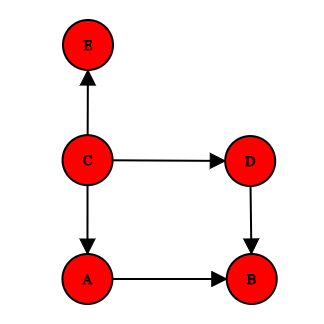
\includegraphics[width=0.45\linewidth]{figures/dag_example.png}
  \caption{Example of a directed acyclic graph}
  \label{fig:dag_example}
\end{figure}

A sequence of arcs connecting two nodes (\textit{end-nodes}) is called a \textit{path} and is denoted with the sequence of nodes $\left(v_{1}, v_{2}, \ldots, v_{n}\right)$ incident on those arcs. A path between two end-nodes is assumed to be unique. If node $v_i$ precedes node $v_j$, there can be no arc from $v_j$ to $v_i$. In this case, $v_i$ is called an \textit{ancestor} of $v_j$ and $v_j$ is called a \textit{descendant} of $v_i$. If these two nodes are adjacent, $v_i$ is called a parent of $v_j$ and $v_j$ is called a child of $v_i$.







\subsection{Bayesian Networks} \label{ssec:bayesian_networks}
% !TEX root = Master.tex

Let $\mathbf{X}=\left\{X_{1}, X_{2}, \ldots, X_{p}\right\}$ be a set of \acp{RV}. A \textit{Bayesian network} is a \ac{DAG} $G = (\bm{V},A)$ where each node $v_i \in \bm{V}$ corresponds to a \ac{RV} $X_i$, $i \in \{1, \ldots, p\}$ and each arc $a = (u,v)$ corresponds to a conditional dependence between two \acp{RV}. The \textit{Markov property}, i.e. a node is conditionally independent of its non-descendants given its parents, enables the representation of the joint probability distribution of the \acp{RV} in $\bm{X}$ as a product of conditional distributions \citep{nagarajan2013bayesian}, allowing simplification of the joint distribution as a result of the \textit{chain rule} and reducing the conditional part to the parents of $X_i$. For discrete \acp{RV}, the joint probability is therefore given by 
\begin{equation}
\mathrm{P}_{\bm{\mathrm{X}}}(\mathbf{X})=
\prod_{i=1}^{p} \mathrm{P}_{X_i}\left(X_{i} \mid X_{1}, \ldots, X_{i-1}\right) =
\prod_{i=1}^{p} \mathrm{P}_{X_{i}}\left(X_{i} \mid \Pi_{X_{i}}\right),
\end{equation}
where $\Pi_{X_{i}}$ is the set of the parents of $X_i$. For continuous \acp{RV}, we can write the joint density of $f_{\mathbf{X}}$ as
\begin{equation}
f_{\mathbf{X}}(\mathbf{X})=
\prod_{i=1}^{p} f_{X_i}\left(X_{i} \mid X_{1}, \ldots, X_{i-1}\right) =
\prod_{i=1}^{p} f_{X_{i}}\left(X_{i} \mid \Pi_{X_{i}}\right).
\end{equation}
\\

In real-world settings, entities often represent variables which vary over time. \textit{\acp{DBN}} extend the framework of static Bayesian networks to model associations arising from temporal dynamics between such entities \citep{nagarajan2013bayesian}. Each \ac{RV} in a \ac{DBN} is represented by several nodes across time-points. In the \ac{DAG} resulting from a \ac{DBN}, arcs can be drawn between variables across successive time-points (or at the same time-point,\footnote{In \cite{nagarajan2013bayesian}) conditional dependencies can occur only between successive time-points. However, this assumption is relaxed here due to practical alignments coming up in Section \ref{ssec:article_dependencies}}, as long as no arc is enters an ancestor node). The arcs in the \ac{DAG} describe exactly the conditional dependencies between any pair of variables given the past variables (or variables at the same time stage). \autoref{fig:dynamic_bn} represents a graphical example of such a \ac{DBN}.
\\


\begin{figure}[H]
\centering
  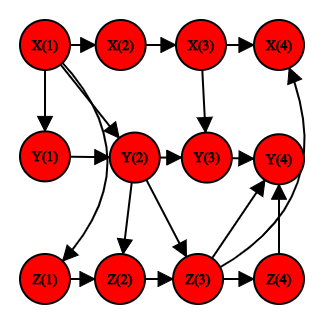
\includegraphics[width=0.45\linewidth]{figures/dynamic_bn.png}
  \caption{Graphical representation of a time-varying dynamic Bayesian network of three random variables ($X$, $Y$ and $Z$) with four time periods}
  \label{fig:dynamic_bn}
\end{figure}


Dependence relationships in \acp{DBN} are often represented by a \ac{VAR} process as in \autoref{eq:multivariate_ts}. Assuming a \ac{VAR}(1) process with $k$ variables, each variable $X_i$, $i = 1,\ldots,k$ satisfies
\begin{equation}
X_{i}(t)=\sum_{j=1}^{k} a_{i j} X_{j}(t-1)+b_{i}+\varepsilon_{i}(t) \quad \text { where } \quad \varepsilon_{i}(t) \sim N\left(0, \sigma_{i}(t)\right),
\end{equation}
where all arcs are defined between two time-points.\footnote{Here consecutive time-points are meant, but this assumption will be relaxed later for practical purposes.} The set of non-zero coefficients $a_{ij}$ in an auto-regressive matrix $A$ define the arc set, meaning that if element $a_{ij}$ is non-zero, the network includes an arc from $X_i$ to $X_j$. Repeated measurements can be used to perform linear regression, however the ordinary least square estimates of the regression coefficients $a_{ij}$ and $b_i$ can be computed only when the number of time-points $n \gg k$.






\newpage
\thispagestyle{empty}
\cleardoublepage

\thispagestyle{plain}
\section{Copulas \& Dependence Structures} \label{sec:copulas_and_dependence_structures}
% !TEX root = Master.tex

Multivariate distributions consist of the marginal distributions and the dependence structure between those marginals. These components can be specified separately in a single framework with the help of copula functions. This chapter introduces the concept of modelling such dependence structures with copulas, which is the main focus of this thesis. The core elements on this subject were picked up from \cite{mcneil2015quantitative}, \cite{Ruppert2015}.
\subsection{Introduction to Copulas} \label{ssec:intro_to_copulas}
% !TEX root = Master.tex

A $d$-dimensional function $C: [0,1]^d \rightarrow [0,1]$ is called a \textit{copula}, if it is a \ac{CDF} with uniform margins, i.e.
\begin{equation*}
P\left(U_{1} \leq u_{1}, \ldots, U_{d} \leq u_{d}\right)=C\left(u_{1}, \ldots, u_{d}\right)
\end{equation*}
where 
$ U_{i}, \hspace{0.25em} i = 1, \ldots, d $ 
are uniformly distributed \acp{RV} in $[0,1]$.\\

\textbf{Probability Transformation}\\
If a \ac{RV} $Y$ has a continuous \ac{CDF} $F$, then
\begin{equation}
F(Y) \sim U[0,1].
\label{eq:probability_transformation}
\end{equation}

\hfill $\square$ \\

The reverse of the \textit{probability transformation} is the \textit{quantile transformation}.\\

\textbf{Quantile Transformation}\\
If $U \sim U[0,1]$ and $F$ be a \ac{CDF}, then
\begin{equation}
P\left(F^{-1}(U) \leq x\right)=F(x)
\label{eq:quantile_transformation}
\end{equation}

\hfill $\square$ \\

The above two transformations allow us to move back and forth between $\mathbb{R}^d$ and $[0,1]^d$ and are the primary building blocks regarding copulas. Against this backdrop, we introduce \textit{Sklar's theorem} which is considered the foundation of all copula related applications.\\




\textbf{Sklar's Theorem} \cite{sklar1959fonctions} \\
Let $F$ be a $d$-dimensional \ac{CDF} with marginal distributions $F_{i}, \hspace{0.25em} i = 1, \ldots, d$.
Then there exists a copula $C$ such that
\begin{equation}
F(x_1, \ldots, x_d) = C (F_1(x_1), \ldots, F_d(x_d))
\label{eq:sklar}
\end{equation}
for all $x_i \in \mathbb{R}, \hspace{0.25em} i = 1, \ldots, d $.\\
The copula $C$ is unique, if $ \hspace{0.25em} \forall i = 1, \ldots, d \hspace{0.25em}$,  $F_i \hspace{0.25em}$  is continuous. Otherwise $C$ is uniquely determined only on
$Ran(F_1) \times \ldots \times Ran(F_d)$, where $Ran(F_{i})$ is the range of $F_i$.\\
Conversely, if $C$ is a $d$-dimensional copula and $F_1, \ldots, F_d$ are univariate \ac{CDF}'s, then $F$ as defined in \autoref{eq:sklar} is a 
$d$-dimensional \ac{CDF}.

\hfill $\square$ \\


If the copula has a \ac{PDF}, then the \textit{copula density} is defined as
\begin{equation}
c(\mathbf{u})=\frac{\partial^{d} C\left(u_{1}, \ldots, u_{d}\right)}{\partial u_{1} \cdots \partial u_{d}} 
\label{eq:copula_density_1}
\end{equation}
for a differentiable copula function $C$ and the realization of a random vector $ \bm{u} = (u_1, \ldots, u_d)$.\\

By virtue of \autoref{eq:sklar} in Sklar's theorem and given that
\begin{equation} 
C(\mathbf{u})=F\left(F_{1}^{-1}\left(u_{1}\right), \ldots, F_{d}^{-1}\left(u_{d}\right)\right) ,
\label{eq:sklar_inverse}
\end{equation}
i.e. inversible \ac{CDF}s $ F_i, \hspace{0.25em} i = 1, \ldots, d, \hspace{0.25em}$ we can rewrite the copula density to
\begin{equation}
c\left(u_{1}, \ldots, u_{d}\right)=\frac{f\left(F_{1}^{-1}\left(u_{1}\right), \ldots, F_{d}^{-1}\left(u_{d}\right)\right)}{\prod \limits _{i=1}^{d} f_{i}\left(F_{i}^{-1}\left(u_{i}\right)\right)}
\label{eq:copula_density_2}
\end{equation}
for densities $f$ of $F$ and $f_1, \ldots, f_d$ of the corresponding marginals.\\


\textbf{Invariance Principal}\\
Suppose the \ac{RV}s $ X_1, \ldots, X_d $  have continuous marginals and copula $C$. For strictly increasing functions $T_i : \mathbb{R} \rightarrow \mathbb{R}, i = 1, \ldots, d$, the \ac{RV}s $T_1(X_1), \ldots, T_d(X_d)$ also have copula $C$.

\hfill $\square$ \\


\textbf{Fr\'echet-Hoeffding Bounds}\\
Let $C(\bm{u}) = C(u_1, \ldots, u_d)$ be any $d$-dimensional copula.\\
Then, for
\begin{equation}
W(\boldsymbol{u})=\max \left\{\sum\limits_{i=1}^{d} u_{i}-d+1, \hspace{0.25em} 0\right\}
\label{eq:frechet_hoeffding_lower}
\end{equation}
as well as
\begin{equation}
M(\boldsymbol{u})=\min \limits _{1 \leq i \leq d}\left\{u_{i}\right\},
\label{eq:frechet_hoeffding_upper}
\end{equation}
it holds that
\begin{equation}
W(\bm{u}) \leq C(\bm{u}) \leq M(\bm{u}), \quad \bm{u} \in[0,1]^{d}.
\label{eq:frechet_hoeffding}
\end{equation}\\
We call $W$ the \textit{lower Fr\'echet-Hoeffding bound} and $M$ the \textit{upper Fr\'echet-Hoeffding bound}.\\
Note that $W$ is a copula if and only if $d=2$, whereas $M$ is a copula for all $d \geq 2$ (more on this later in Section \ref{sssec:fundamental_copulas}).

\hfill $\square$ \\


MORE ON COPULA THEORY (NOTES)




\subsection{Copula Classes} \label{ssec:copula_classes}
% !TEX root = Master.tex

In this section we will take a look at three very popular \textit{copula classes}, namely \textit{fundamental, elliptical and archimedean copulas}. For each class, a few (parametric) \textit{copula families}, which are widely used, will be presented.
\subsubsection{Fundamental Copulas} \label{sssec:fundamental_copulas}
% !TEX root = Master.tex

Fundamental copulas are a basic class of copulas, which emerge directly from the copula framework and do not depend on any parametric components. \\

\textbf{Independence Copula}\\
It is well known that the joint \ac{CDF} of a finite set of \acp{RV}
$X_i, i = 1, \ldots, n$, is equal to the product of the margins if and only if the \acp{RV} $X_i$ are mutually independent, i.e.
\begin{equation}
F_{X_{1}, \ldots, X_{n}}\left(x_{1}, \ldots, x_{n}\right)= \prod_{i=1}^{n} F_{X_{i}}\left(x_{i}\right)) \quad \forall x_1, \ldots, x_n.
\end{equation}

Equally, the exact same concept applies when we talk about the \textit{independence copula}, i.e.
\begin{equation}
\Pi (\bm{u}) = \prod \limits _{i = 1}^d u_i.
\end{equation}
As a result of Sklar's theorem, the \ac{RV}s $u_i$ are independent if and only if their copula is the independence copula, i.e.
\begin{equation}
 C(\bm{u}) = \Pi (\bm{u}) 
 \end{equation}
and thus the copula density would be 
\begin{equation}
c(\boldsymbol{u})=1, \quad \boldsymbol{u} \in[0,1]^{d}.
\end{equation}

%From \autoref{eq:frechet_hoeffding}, it is obvious that the Fr\'echet-Hoeffding bounds correspond to the extreme cases of perfect dependence between the \ac{RV}s $X_i, i = 1, \ldots, d$. \\

%\textbf{Comonotonicity Copula}\\
%Consider the \ac{RV}s $X_1, \ldots, X_d$ and strictly increasing transformations $T_1, \ldots, T_d$ and $X_i = T(X_i)$ for $i = 2, \ldots, d$. Making use of the \textit{invariance principal}, it can be shown that these \ac{RV}s have as copula the upper Fr\'echet-Hoeffding bound 
%$$M(\bm{u}) = \min\{ u_1, \ldots, u_d \}.$$ Since there is perfect positive dependence between those \ac{RV}s, $M$ is called the \textit{comonotonicity copula}. The number of dimensions $d$ can be any finite number greater than or equal to $2$ for $M$ to be a copula, as the minimum remains well defined.
%
%
%
%
%\textbf{Countermonotonicity Copula}\\
%Similar to the comonotonic case, it can be shown that if two \acp{RV} $X_1$ and $X_2$ are perfectly negatively dependent, their copula is the lower Fr\'echet-Hoeffding bound
%$$
%W(\boldsymbol{u})=\max \left\{\sum\limits_{i=1}^{d} u_{i}-d+1, \hspace{0.25em} 0\right\}.
%$$
%Therefore, $W$ is known as the \textit{countermonotonicity copula}. Because of the fact that countermonotonicity is not valid for a dimension greater than $2$, we end up with the restriction $d=2$ for $W$ to be indeed a copula.









\subsubsection{Elliptical Copulas} \label{sssec:elliptical_copulas}
% !TEX root = Master.tex

Copulas which can be derived from known multivariate distributions like for example the \textit{Multivariate Normal (or Gaussian) Distribution} or the \textit{Multivariate Student's t-Distribution} are called \textit{implicit copulas}. \textit{Elliptical copulas} are implicit copulas which arise via Sklar's theorem from elliptical distributions like the mentioned examples.\\

\textbf{Gaussian Copula}\\
Without loss of generality, for a random vector $\bm{X} \sim {\mathcal{N}_{d}(\bm{0}, \mathbf{P})} $ and \textit{correlation matrix} $\bm{P}$,
the \textit{Gaussian copula (family)} is given by
\begin{equation}
C_{\mathbf{P}}^{G a}(\mathbf{u})=\Phi_{\mathbf{P}}\left(\Phi^{-1}\left(u_{1}\right), \ldots, \Phi^{-1}\left(u_{d}\right)\right),
\end{equation}
where $\Phi$ is the \ac{CDF} of $\mathcal{N}(0, \sigma^{2})$ and 
$\Phi_{\bm{P}}$ is the \ac{CDF} of $\mathcal{N}_{d}(\bm{0}, \mathbf{P})$.\\
There are special cases to this copula family, namely for $d=2$ and correlation $\rho$, the \textit{bivariate Gaussian copula} $C_{\rho}^{G a}$ is equivalent to
\begin{itemize}
\item the independence copula $\Pi$ if $\rho = 0$,
\item the comonotonicity copula $M$ if $\rho = 1$ and
\item the countermonotonicity copula $W$ if $\rho = -1$
\end{itemize}
The density of the Gaussian copula is given by
\begin{equation}
c_{\bm{P}}^{\mathrm{Ga}}(\boldsymbol{u})=\frac{1}{\sqrt{\operatorname{det} \bm{P}}} \exp \left(-\frac{1}{2} \boldsymbol{x}^{\prime}\left(\bm{P}^{-1}-\bm{I}_{d}\right) \boldsymbol{x}\right),
\end{equation}
where $\bm{x} = \left(\Phi^{-1}\left(u_{1}\right), \ldots, \Phi^{-1}\left(u_{d}\right)\right)$.

\hfill $\square$ \\




 \begin{figure}[H]
\centering
\begin{subfigure}{.45\textwidth}
  \centering
  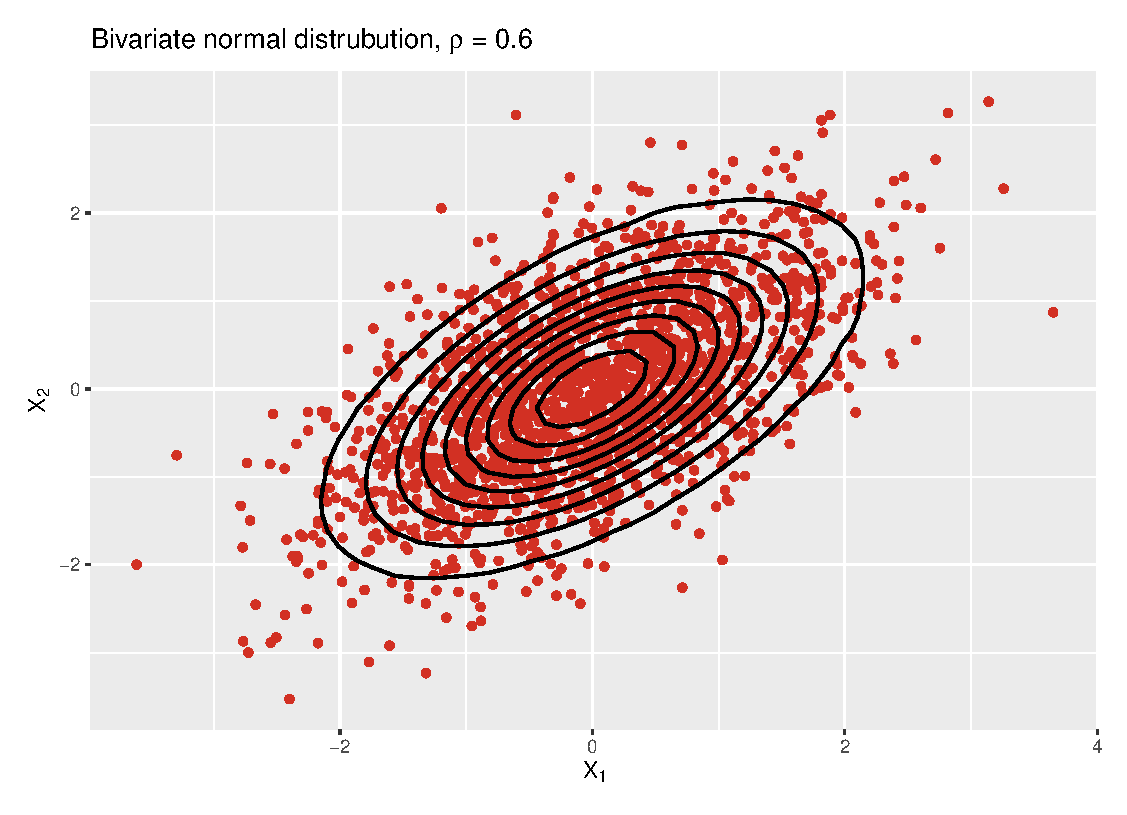
\includegraphics[width=\linewidth]{figures/bivariate_normal.eps}
  \caption{Gaussian distribution with contour lines}
  \label{fig:mvd_normal_copula}
\end{subfigure}
\begin{subfigure}{.45\textwidth}
  \centering
  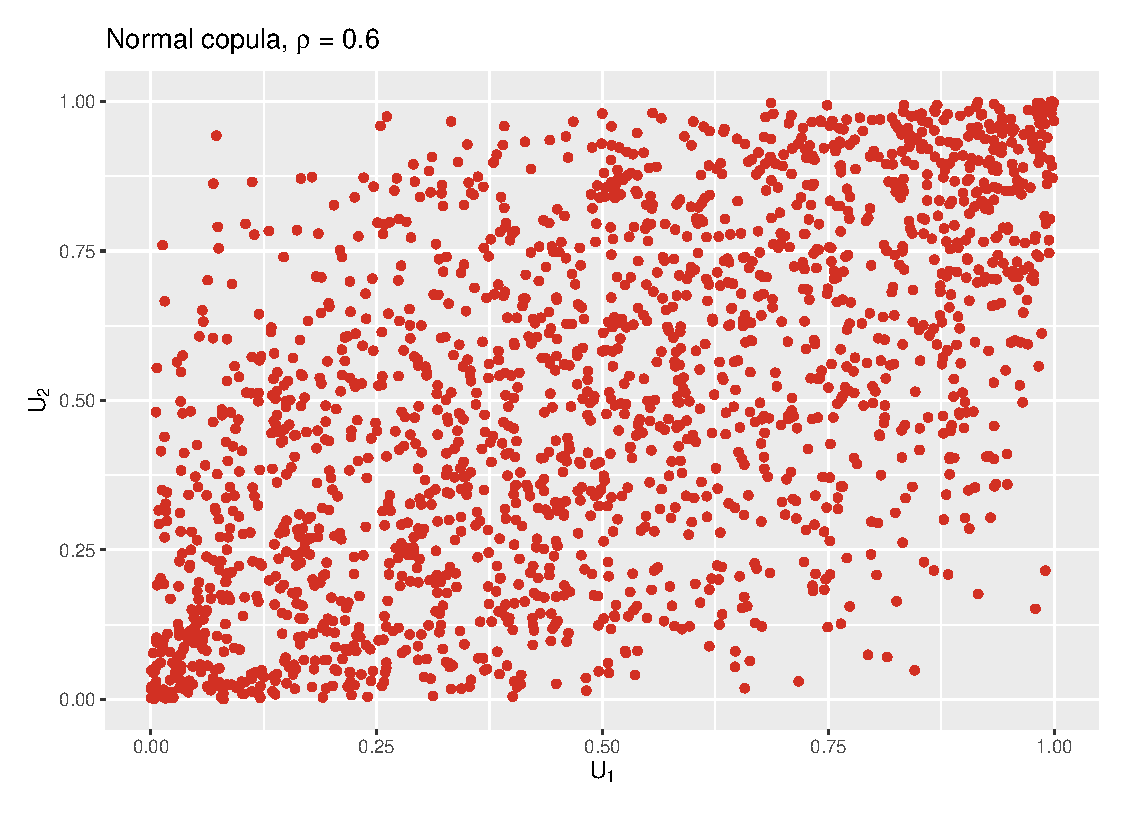
\includegraphics[width=\linewidth]{figures/normal_copula.eps}
  \caption{Gaussian copula}
  \label{fig:normal_copula}
\end{subfigure}
\caption{Bivariate Gaussian distribution and Gaussian copula for Pearson's $\rho = 0.6$ and simulated sample of size $n = 1800$, both with standard normal marginals}
\label{fig:normal_plots}
\end{figure}






\textbf{t-Copula}\\
Consider without loss of generality $\bm{X} \sim {t_{d}(\nu, \bm{0}, \mathbf{P})}$ (multivariate Student's t-distribution) with $\nu$ \ac{dof} and $\bm{P}$ a correlation matrix, then the \textit{t-copula (family)} is given by
\begin{equation}
C_{\nu, \bm{P}}^{t}(\mathbf{u})=t_{\nu, \bm{P}}\left(t_{\nu}^{-1}\left(u_{1}\right), \ldots, t_{\nu}^{-1}\left(u_{d}\right)\right),
\end{equation}
where $t_{\nu}$ is the \ac{CDF} of the univariate Student's t-distribution  and $t_{\nu, \bm{P}}$ is the \ac{CDF} of the multivariate Student's t-distribution (both with $\nu$ \ac{dof}).\\
For the \textit{bivariate t-copula} ($d=2$), the special cases are the same as for the Gaussian copula except that $d=0$ does not yield the independence copula (unless $\nu \rightarrow \infty$ in which case  $ C_{\nu, \rho}^{t} = C_{\rho}^{G a}$).\\
The density of $C_{\nu, \bm{P}}^{t}$ is given by
\begin{equation}
c_{\nu, \mathbf{P}}^{t}(\boldsymbol{u})=\frac{\Gamma((\nu+d) / 2)}{\Gamma(\nu / 2) \sqrt{\operatorname{det} \mathbf{P}}}\left(\frac{\Gamma(\nu / 2)}{\Gamma((\nu+1) / 2)}\right)^{d} \frac{\left(1+\boldsymbol{x}^{\prime} \mathbf{P}^{-1} \boldsymbol{x} / \nu\right)^{-(\nu+d) / 2}}{\prod_{j=1}^{d}\left(1+x_{j}^{2} / \nu\right)^{-(\nu+1) / 2}},
\end{equation}
where $\bm{x} = \left(t_{\nu}^{-1}\left(u_{1}\right), \ldots, t_{\nu}^{-1}\left(u_{d}\right)\right)$.

\hfill $\square$ \\






 \begin{figure}[H]
\centering
\begin{subfigure}{.45\textwidth}
  \centering
  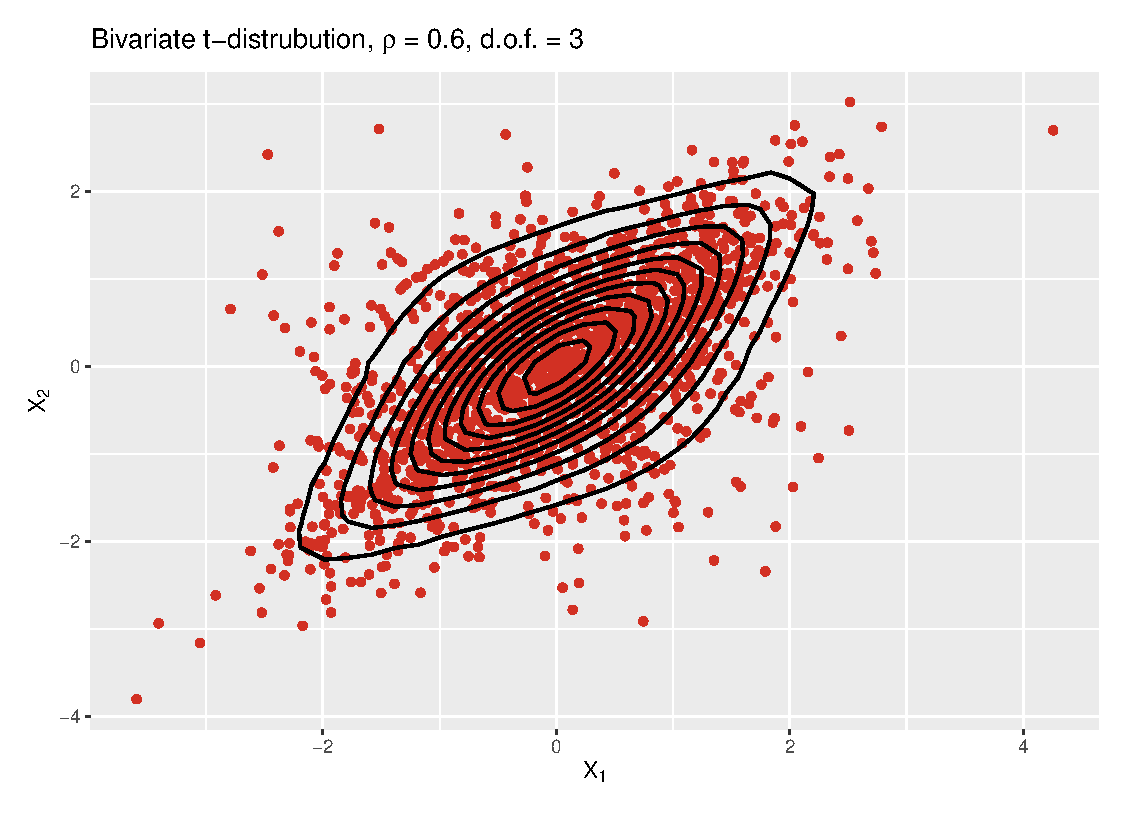
\includegraphics[width=\linewidth]{figures/bivariate_t.eps}
  \caption{t-distribution with contour lines}
  \label{fig:bivariate_t}
\end{subfigure}
\begin{subfigure}{.45\textwidth}
  \centering
  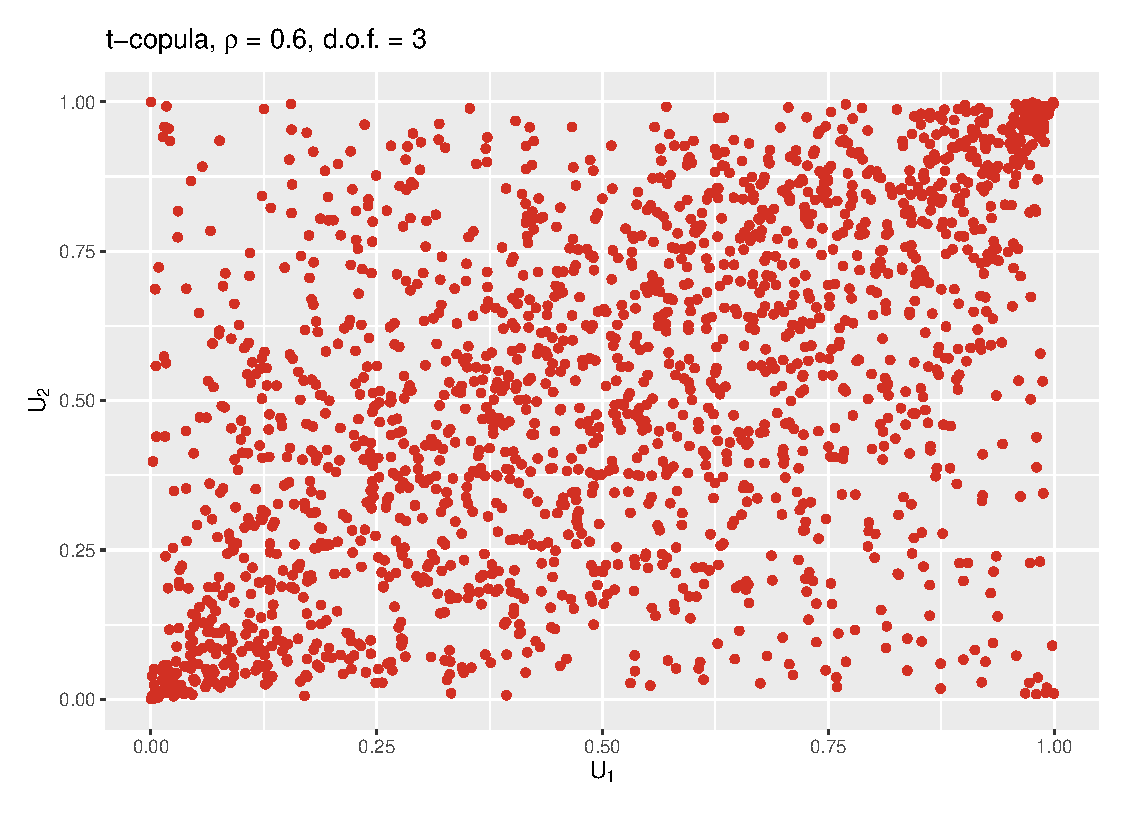
\includegraphics[width=\linewidth]{figures/t_copula.eps}
  \caption{t-copula}
  \label{fig:t_copula}
\end{subfigure}
\caption{Bivariate t-distribution and t-copula with 3 degrees of freedom for Pearson's $\rho = 0.6$ and simulated sample of size $n = 1800$, both with standard normal marginals}
\label{fig:t_plots}
\end{figure}







\subsubsection{Archimedean Copulas} \label{sssec:archimedean_copulas}
% !TEX root = Master.tex

Unlike implicit copulas, \textit{explicit copulas} can be specified directly by taking into account certain constructional principles. The most important aspects of a such explicit copulas, in particular \textit{archimedean copulas}, are showcased in this subsection. Archimedian copulas are of the general form
\begin{equation}C(\boldsymbol{u})=\psi\left(\psi^{-1}\left(u_{1}\right)+\cdots+\psi^{-1}\left(u_{d}\right)\right),
\label{eq:archimedean_generator}
\end{equation}
where the function $\psi:[0, \infty) \rightarrow[0,1]$ is the \textit{(archimedean) generator} and satisfies the following properties:
\begin{itemize}
\item $\psi$ is strictly decreasing in the entire domain $[0, \infty)$
\item $\psi (0) = 1$
\item $\psi(\infty)=\lim \limits _{t \rightarrow \infty} \psi(t)=0$
\item We set $\psi^{-1}(0)=\inf \{t: \psi(t)=0\}$
\end{itemize}
If $\psi(t)>0, t \in[0, \infty)$, we call $\psi$ \textit{strict}. The set of all generators is denoted by $\Psi$.\\
Based on \autoref{eq:archimedean_generator} and the generator, we can construct several copula families. Three of the most popular ones are the \textit{Gumbel}, the \textit{Clayton} and the \textit{Frank} \textit{copula}.





\subsection{Dependence Measures} \label{ssec:dependence_measures}
% !TEX root = Master.tex

\textit{Dependence measures} allow us to summarize a particular kind of dependence into a single number.\footnote{In the bivariate case} Recall the Fr\'echet-Hoeffding bounds (\autoref{eq:frechet_hoeffding_lower} and \autoref{eq:frechet_hoeffding_upper}). They are an example of such kind of dependence measures. After all, they represent perfect negative or positive dependence.
In this section, we will take a closer look into three classes of dependence measures along with appropriate association metrics.


\subsubsection{Linear Correlation} \label{sssec:linear_correlation}
% !TEX root = Master.tex

Undoubtedly, the most famous association metric for two \acp{RV} $X_1$ and $X_2$ is the \textit{Linear or Pearson's correlation coefficient}
\begin{equation}
\rho\left(X_{1}, X_{2}\right)=
\frac{\operatorname{Cov}\left(X_{1}, X_{2}\right)}{\sqrt{\operatorname{Var} (X_{1})} \sqrt{\operatorname{Var} (X_{2})}}
\in [-1, 1].
\label{eq:pearsons_rho}
\end{equation}
Note that $E(X_1) < \infty$ and $E(X_2) < \infty$ have to hold, i.e. the first two moments have to exist for $\rho$ to be defined.\\
The Pearson correlation coefficient is interpretable for \acp{RV} which have (approximately) a linear relationship, where $\rho = -1$ indicates perfect negative linear correlation, $\rho=1$ indicates perfect positive linear correlation and $\rho=0$ indicates no correlation between $X_1$ and $X_2$. However, comprehensibility of this measure comes along with some drawbacks:
\begin{itemize}
\item A correlation of $0$ is in general not equivalent to independence. This property holds only for normally distributed \acp{RV}.\footnote{e.g. $X_2 =X_1^2$ implies perfect dependence, yet $\rho(X_1,X_2) = 0$. Conversely though, independence always yields $\rho=0$.}
\item $\rho$ is invariant only under linear transformations, but not under transformations in general.
\item Given the marginals and correlation $\rho$, one is able to construct a joint distribution only for the class of elliptical distributions. (MAYBE PLOT qrm)
\item Given the marginals, only for elliptically distributed \acp{RV} any $\rho \in [-1,1]$ is attainable.
\end{itemize}









\subsubsection{Rank Correlation} \label{sssec:rank_correlation}
% !TEX root = Master.tex

To compensate some of the drawbacks of linear correlation, we can take advantage of correlation measures based on the ranks of data. \textit{Rank correlation coefficients}, like the ones presented below, are always defined and obey to the invariance principal. This means that these coefficients only depend on the underlying copula and they can thereof be directly derived.\\

\textbf{Spearman's Rho}\\
Consider two \acp{RV} $X_1$ and $X_2$ with continuous \acp{CDF} $F_1$ and $F_2$, then the \textit{Spearman's rho correlation coefficient} is simply the linear correlation between the \acp{CDF}
\begin{align}
\rho_{S}=\rho\left(F_{1}\left(X_{1}\right), F_{2}\left(X_{2}\right)\right).
\end{align}
The reason being is that by applying the \ac{CDF} to data, naturally a multiple of the ranks of the data are obtained, which essentially is equivalent to
\begin{equation}
\rho_S = \rho ( Ran(X_1), Ran(X_2) )
\end{equation}
Due to the invariance principle, we also obtain Spearman's rho directly from the unique copula via
\begin{equation}
\rho_{\mathrm{S}}=12 \int_{0}^{1} \int_{0}^{1} C\left(u_{1}, u_{2}\right) \mathrm{d} u_{1} \mathrm{d} u_{2}-3.
\end{equation}


\textbf{Kendall's Tau}\\
Let $X_1 \sim F_1$ and $X_2 \sim F_2$ be two \ac{RV} and let $(\tilde{X}_{1}, \tilde{X}_{2})$ be an independent copy\footnote{An independent copy $\tilde{X}$ of a RV $X$ is a RV that inherits from the same distribution as $X$ and is independent of $X$.} of $({X}_{1}, {X}_{2})$. Then \textit{Kendall's tau} is defined by 
\begin{equation}
\begin{aligned}
\rho_{\tau} &={E}\left[\operatorname{sign}\left(\left(X_{1}-X_{1}^{\prime}\right)\left(X_{2}-X_{2}^{\prime}\right)\right)\right] \\
&={P}\left(\left(X_{1}-X_{1}^{\prime}\right)\left(X_{2}-X_{2}^{\prime}\right)>0\right)-{P}\left(\left(X_{1}-X_{1}^{\prime}\right)\left(X_{2}-X_{2}^{\prime}\right)<0\right).
\end{aligned}
\end{equation}
Similarly to Spearman's rho, using the invariance principal, we can directly derive Kendall's tau from the unique copula by
\begin{equation}
\rho_{\tau}\left(X_{1}, X_{2}\right)=4 \int_{0}^{1} \int_{0}^{1} C\left(u_{1}, u_{2}\right) d C\left(u_{1}, u_{2}\right)-1.
\label{eq:kendall_to_copula}
\end{equation}


Both $\rho_S, \rho_{\tau} \in [-1,1]$ and any value within this interval is attainable for an arbitrary copula class in contrast to the Pearson coefficient. 
If any of these rank correlations is -1 (or 1), we are in the countermonotonic (or comonotonic) case. If $\rho_S$ (or $\rho_{\tau}$) $=0$, this does not necessarily imply independence between $X_1$ and $X_2$, although the opposite direction holds.
Furthermore, they are not limited to be invariant just under linear transformations . 











\subsubsection{Tail Dependence} \label{sssec:tail_dependence}
% !TEX root = Master.tex

\textit{Coefficients of tail dependence} express the strength of the dependence in the extremes of distributions, i.e. the joint tails. We distinguish between \textit{lower} and \textit{upper tail dependence} between $X_j \sim F_j, j = 1,2$ and provided that the below limits exist, they are given by
\begin{equation}
\lambda_{l}=\lim \limits _ {q \rightarrow 0^+} P \left(X_{2} \leq F_{2}^{\leftarrow}(q) | X_{1} \leq F_{1}^{\leftarrow}(q)\right) 
\label{eq:lower_tail_dependence}
\end{equation}
and 
\begin{equation}
\lambda_{u}=\lim \limits _ {q \rightarrow 1^-} P \left(X_{2} > F_{2}^{\leftarrow}(q) | X_{1} > F_{1}^{\leftarrow}(q)\right).
\label{eq:upper_tail_dependence}
\end{equation}
If $\lambda_l$ (or $\lambda_u$) $=0$, then we say that $X_1$ and $X_2$ are \textit{asymptotically independent} in the lower (or upper) tail,\footnote{Not necessarily true for the other way around} otherwise we have lower (or upper) tail dependence.\\
For continuous \acp{CDF} and by using Bayes' theorem, these expressions can be re-written to
$$
\begin{aligned}
\lambda_{l} &=\lim _{q \rightarrow 0^+} \frac{P\left(X_{2} \leq F_{2}^{\leftarrow}(q), X_{1} \leq F_{1}^{\leftarrow}(q)\right)}{P\left(X_{1} \leq F_{1}^{*}(q)\right)} \\
&=\lim _{q \rightarrow 0^+} \frac{C(q, q)}{q}
\end{aligned}
$$
and similarly
$$
\lambda_u = 2-\lim _{q \rightarrow 1^-} \frac{1-C(q, q)}{1-q}.
$$
Therefore, tail dependencies can be assessed by means of the copula itself when approaching the points $(0,0)$ and $(1,1)$. In addition, for all radially symmetric copulas (e.g. the bivariate Gaussian or the t-copula) we have $\lambda_l = \lambda_u = \lambda$.\\
Some examples are:
\begin{itemize}
\item Clayton: $\lambda_l = 2^{-1/ \theta}$, $\lambda_u = 0$ (only lower tail dependence)
\item Gumbel: $\lambda_l = 0$, $\lambda_u = 2 - 2^{1/ \theta}$ (only upper tail dependence)
\item Frank: $\lambda_l = 0$, $\lambda_u = 0$ (no tail dependence)
\end{itemize}
Following such guidelines, the choice of a practicable copula can be facilitated.





\subsection{Structured Additive Conditional Copulas} \label{ssec:conditional_copulas}
% !TEX root = Master.tex

Modelling of the marginal response distributions along with their dependence structure has been studied so far in a strictly parametric context, not considering any potentially available covariate information. In this section, the copula framework will be broadened by adding conditions given possible covariates for all model parameters, i.e. both for the parameters of the margins as well as the copula parameter. All involved model parameters will receive \textit{structured additive predictors} (see Section \ref{ssec:gam}) to account for possible non-linear or random effects. We will summarily explore \textit{Structured Additive Conditional Copulas} and for extensive literature, good references to view are \cite{klein2016simultaneous}, \cite{vatter2019gamcopula} and \cite{marra1605bivariate}. \\

To get started, we define $(Y_1, Y_2)'$ to be independent bivariate responses and $\bm{\nu}$ being the information contained in covariates. Ergo, \autoref{eq:sklar} of Sklar's theorem can be extended to the conditional case
\begin{equation}
F_{1,2}\left(Y_{1}, Y_{2} | \bm{\nu} \right)=C\left(F_{1}\left(Y_{1} | \bm{\nu} \right), F_{2}\left(Y_{2} | \bm{\nu} \right) | \bm{\nu} \right)
\label{eq:sklar_conditional}
\end{equation}
in conjunction with all facets of Section \ref{ssec:intro_to_copulas} \citep{patton2006modelling}.\\
The marginal \acp{CDF} $F_{d}\left(y_{i d} | \bm{\nu}_i\right)$ for observations $i = 1,\ldots, n$ can also be stated as
\begin{equation}
F_{d}\left(y_{i d} | \vartheta_{i 1}^{(d)}, \ldots, \vartheta_{i K_{d}}^{(d)}\right), \quad d = 1, 2,
\end{equation}
i.e. the distribution $F_d$ has a total of $K_d$ parameters, denoted as $\vartheta_{i 1}^{(d)}, \ldots, \vartheta_{i K_{d}}^{(d)}$.
To relate all parameters of the margins to structured additive predictors $\eta_i^{\vartheta_k^{(d)}},  k = 1,\ldots, K_d$ consisting of the covariates $\bm{\nu}_i$ (see Section \ref{ssec:gam}), we employ strictly increasing response mappings $h_k^{(d)}$ to ensure proper domain allocation, i.e.
\begin{equation}
\vartheta_{i k}^{(d)}=h_{k}^{(d)}(\eta_{i}^{\vartheta_{k}^{(d)}}).
\label{eq:parameter_mapping}
\end{equation}
\\

Assuming that the parameters of the copula can also depend on covariates $\bm{\nu}_i$ while Sklar's theorem applies as usual, the left-hand side of \autoref{eq:sklar_conditional} can equivalently be stated as  
$$
F_{1,2}(y_{i 1}, y_{i 2} | v_{i})= F_{1,2}(y_{i 1}, y_{i 2} | \vartheta_{i 1}^{(1)}, \ldots, \vartheta_{i K_{1}}^{(1)}, \vartheta_{i 1}^{(2)}, \ldots,
\vartheta_{i K_{2}}^{(2)}, \vartheta_{i 1}^{(c)}, \ldots, \vartheta_{i K_{c}}^{(c)}),
$$
where the last share of parameters $\vartheta_{i 1}^{(c)}, \ldots, \vartheta_{i K_{c}}^{(c)}$ belong to the copula. Similar to \autoref{eq:parameter_mapping}, the copula parameters are modelled as $\vartheta_{i k}^{(c)}=h_{k}^{(c)}(\eta_{i}^{\vartheta_{k}^{(c)}})$ with $K_c$ being the number of parameters.














%\subsection{Vine Copulas} \label{ssec:vine_copulas}
%% !TEX root = Master.tex

Vine copulas to be written down... 

\newpage
\thispagestyle{empty}
\cleardoublepage


\thispagestyle{plain}
\section{Data Exploration} \label{sec:data_exploration}
% !TEX root = Master.tex

In Section \ref{ssec:data_sources} we introduced the setup of the data to be treated. As one can see in \autoref{tab:article_master_data}, each article can be assigned to a set of attributes. Besides some elemental attributes like \textit{color}, \textit{age group} or \textit{gender}, the data exhibit a "natural" company-specific hierarchical structure. In \autoref{fig:article_hierarchy}, we can see an example of such a hierarchy for the attributes \textit{business unit} and \textit{product division}. The bottom level consists of the articles themselves and at the top level we have the brand. Note that the brand \textit{Reebok} also belongs to adidas-group, but we are only concerned with adidas products within the scope of this thesis. 

\begin{figure}[H]
\centering
  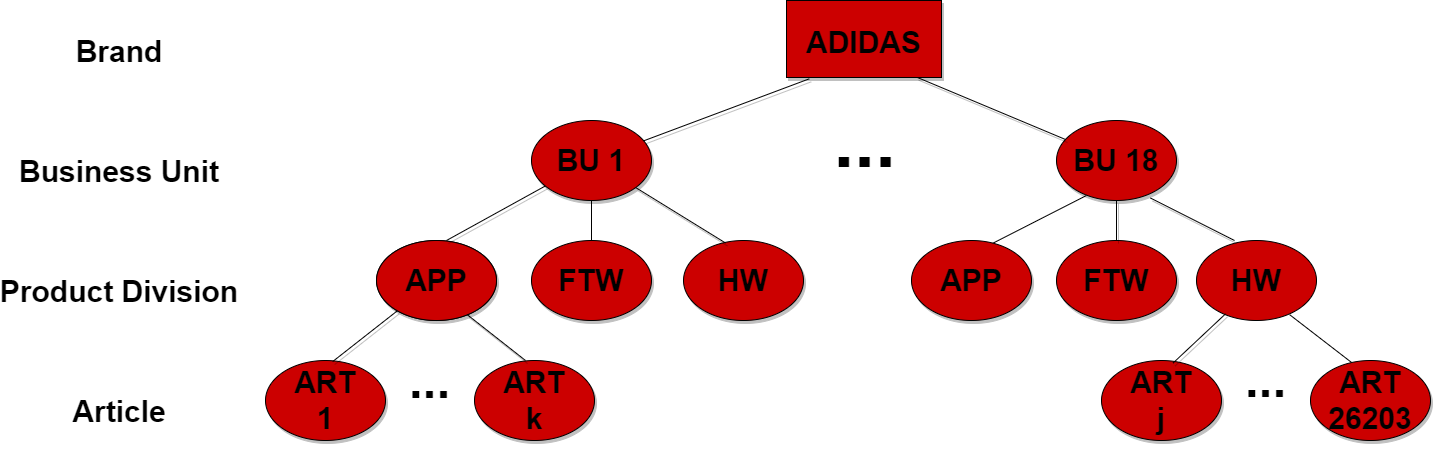
\includegraphics[width=.95\linewidth]{figures/article_tree_white.png}
  \caption{Illustration of the article's hierarchical structure using only a fraction of attributes: brand, business unit, product division (APP: Apparel, FTW: Footwear, HW: Hardware), articles.}
  \label{fig:article_hierarchy}
\end{figure}







\subsection{Universal Sale Patterns} \label{ssec:universal_patterns}
% !TEX root = Master.tex



As mentioned in Section \autoref{ssec:data_sources}, the data contain the information about sold articles over the years 2017 and 2018. \autoref{fig:total_sold_articles_ts} shows the weekly course for the quantities over those two years, highlighting active promotion weeks as vertical lines. We can undoubtedly recognize that \textit{"Black Friday"} weeks (black vertical lines) have an exceptional impact on sales, as they stand internationally for the most busy shopping periods. During these days in mid- to late November each year, large amounts of different products are heavily discounted.
\\

\begin{figure}[H]
\centering
  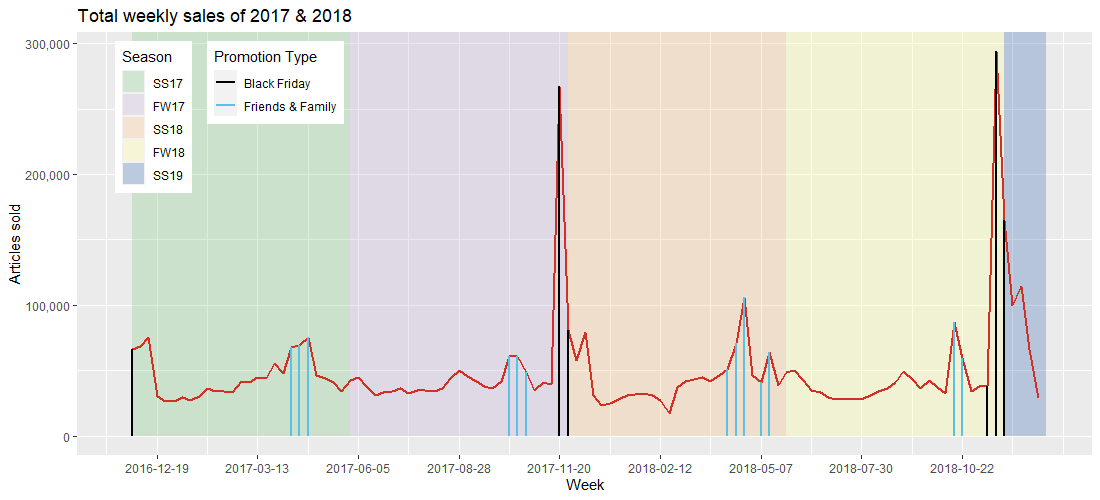
\includegraphics[width=1\linewidth]{figures/total_sold_articles_ts.png}
  \caption{Course of article unit sales}
  \label{fig:total_sold_articles_ts}
\end{figure}

Another promotion type we are interested in is \textit{"Friends \& Family"}, occurring yearly around April-May and October, where on the eCom website plenty of articles are on offer. On these weeks, we have elevated numbers of sold articles as well (blue vertical lines).
\\

Tables \ref{tab:black_friday} and \ref{tab:friends_and_family} show the weeks were Black Friday and Friends \& Family took place respectively. The dates on those tables are one week apart each and always indicate the Monday of the respective week\footnote{According to European standards, a week starts on Monday.}. 
\\


\begin{table}[H]
\setlength\arrayrulewidth{1pt}  
\centering
\begin{adjustbox}{max width=\textwidth}

\
\begin{tabular}{|
>{\columncolor{lightgray}}c |c|c|c|c|c|c|}
\hline
\textbf{Black Friday weeks} & 2016-11-28 & 2017-11-20 & 2017-11-27 & 2018-11-12 & 2018-11-19 & 2018-11-26 \\ \hline
\end{tabular}

\end{adjustbox}
\caption{Black Friday weeks}
\label{tab:black_friday}
\end{table}




\begin{table}[H]
\setlength\arrayrulewidth{1pt}  
\centering
\begin{adjustbox}{max width=\textwidth}

\
\begin{tabular}{|
>{\columncolor{lightgray}}c |c|c|c|c|c|c|c}
\hline
\cellcolor{lightgray}                                              & 2017-04-10 & 2017-04-17 & 2017-04-24 & 2017-10-09 & 2017-10-16 & 2017-10-23 & \multicolumn{1}{l|}{2018-04-09} \\ \cline{2-8} 
\multirow{-2}{*}{\cellcolor{lightgray}\textbf{Friends \& Family weeks}} & 2018-04-16 & 2018-04-23 & 2018-05-07 & 2018-05-14 & 2018-10-15 & 2018-10-22 &            \\ \cline{1-7}
\end{tabular}

\end{adjustbox}
\caption{Friends \& Family weeks}
\label{tab:friends_and_family}
\end{table}

\autoref{fig:promos_against_sales} depicts scatterplots of 10,000 randomly chosen observations in the dataset, where the two main promotion intensities are plotted against article unit sales. An overall positive relationship is visible as we would expect, even more so for Black Friday. Due to the huge noise persisting in these relationships however, Pearson's correlation coefficient for Black Friday against sales and Friends \& Family against sales take on values of 0.32 and 0.11 respectively. Notice the high concentration of different sale quantities when there is neither Black Friday nor Friends \& Family promotion activity (vertical points on the y-axes of \autoref{fig:promos_against_sales}). Similar behavioural conclusions can be made about the total markdown percentage, with a correlation coefficient of 0.27 (see \autoref{fig:markdown_against_logsales}). The type of season (Fall-Winter (FW) or Spring-Summer (SS)) doesn't seem to make an overall difference in the sale quantities, as a glimpse at \autoref{fig:season_type_against_logsales} points out (at least for modelling purposes as will be discussed in Chapter \ref{sec:modelling}). 
\\

 \begin{figure}[H]
\centering
\begin{subfigure}{.45\textwidth}
  \centering
  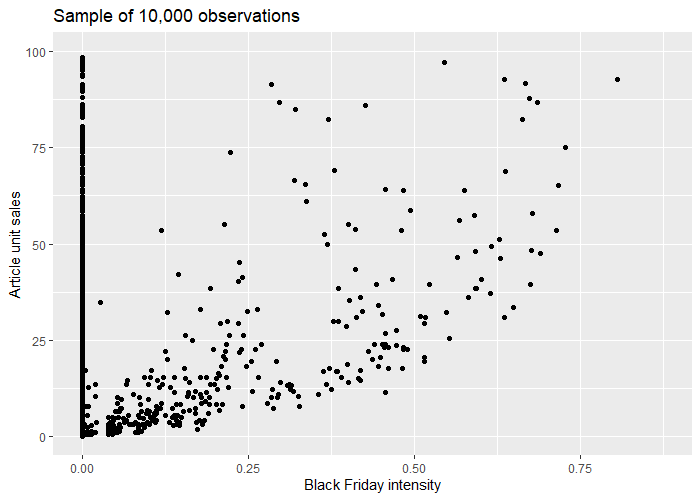
\includegraphics[width=\linewidth]{figures/bf_against_sales.png}
  \caption{Black Friday against unit sales}
  \label{fig:bf_against_sales}
\end{subfigure}
\begin{subfigure}{.45\textwidth}
  \centering
  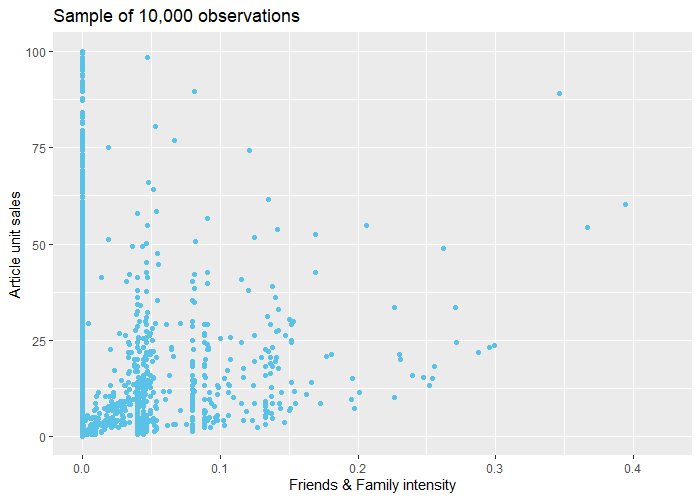
\includegraphics[width=\linewidth]{figures/ff_against_sales.png}
  \caption{Friends \& Family against unit sales}
  \label{fig:ff_against_sales}
\end{subfigure}
\caption{Scatterplots of promotion intensities against article unit sales; The y-axes are cut at 100}
\label{fig:promos_against_sales}
\end{figure}



 \begin{figure}[H]
\centering
  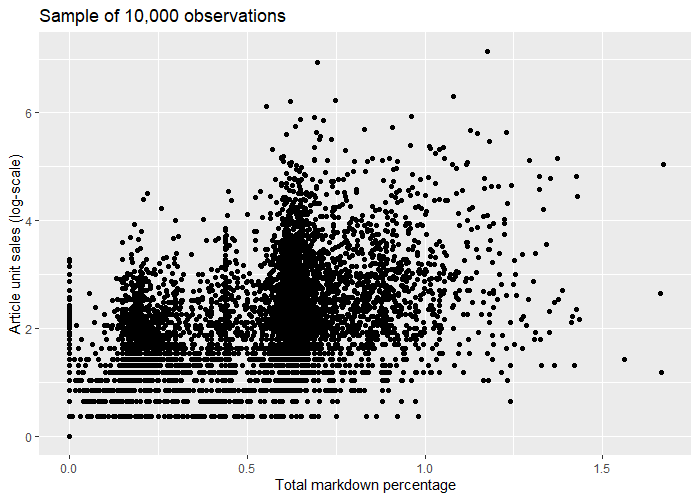
\includegraphics[width=0.65\linewidth]{figures/markdown_against_logsales.png}
  \caption{Unit sales in log-scale against total markdown percentage}
  \label{fig:markdown_against_logsales}
\end{figure}



 \begin{figure}[H]
\centering
  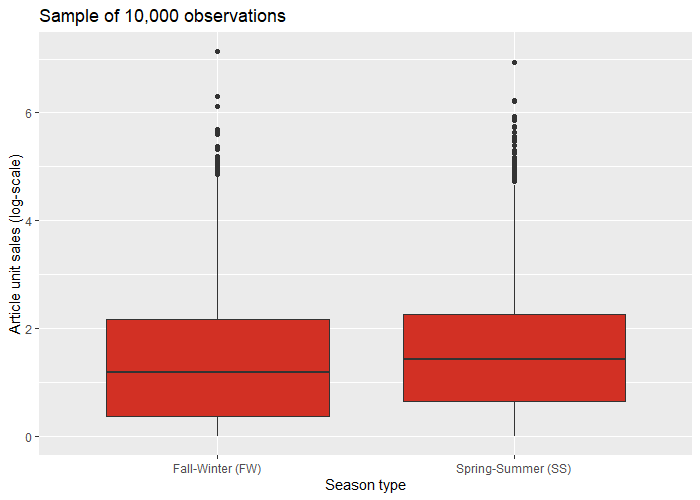
\includegraphics[width=0.65\linewidth]{figures/season_type_against_logsales.png}
  \caption{Unit sales in log-scale against season type}
  \label{fig:season_type_against_logsales}
\end{figure}





Regarding the months, they don't seem to differ much in their sale quantities, that is of course excluding the months of the two mentioned promotion types. The monthly sales portions for those months can be observed in \autoref{fig:sales_without_promo_months}. We have slightly higher sale portions on January, June and July. 
Most probably this is due to Christmas and "end of the year" shopping habits, which are carried forward from December to the very next month January. 
Regarding June and July, they indicate summer periods and frequent occurrence of big sports events, which may drive sales. 
Notice that, despite the fact that December is not explicitly present in \autoref{tab:black_friday}, it is nonetheless a Black Friday month as the promotion is still activated moving from November to December (see \autoref{fig:monthly_ts}). 
\\


 \begin{figure}[H]
\centering
\begin{subfigure}{.45\textwidth}
  \centering
  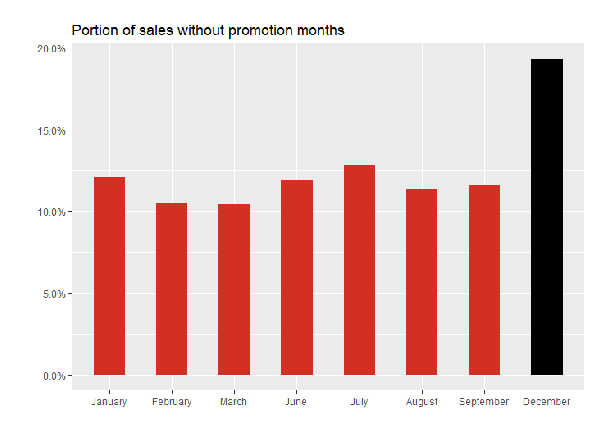
\includegraphics[width=\linewidth]{figures/sales_without_promo_months.eps}
  \caption{Sales distribution grouped by months without promos}
  \label{fig:sales_without_promo_months}
\end{subfigure}
\begin{subfigure}{.45\textwidth}
  \centering
  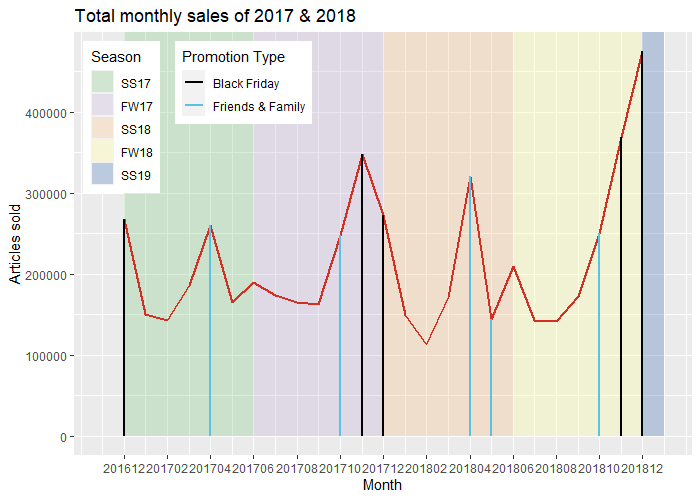
\includegraphics[width=\linewidth]{figures/monthly_ts.png}
  \caption{Monthly course of article unit sales with promo indicators}
  \label{fig:monthly_ts}
\end{subfigure}
\caption{Monthly patterns of article unit sales}
\label{fig:monthly_sales}
\end{figure}



Moving forward, reviewing some sale summary statistics along with the findings so far, we detect a very high overdispersion in our data. The first two rows in \autoref{tab:quantiles_sold_units_week} give as a first impression of the sales' distribution. Considering the sold units of one article at a time within a week, there are lots of weeks where no single unit was sold. The median is at 2.71 units,\footnote{Reminder from Section \ref{ssec:data_sources}: the values are in reality discrete, but due to anonymization they were transformed into real numbers.} 75\% of the "article-week" combinations take on a value of at most 20 and the minority exceeds 100 pieces (99\%-quantile). The third row of the table shows how many distinct articles fall under the respective quantile of sales and there is a visible anti-proportional behaviour towards the number of sold units, which is of course intuitive. Remarkable though is the quantity of affected articles even for incredibly large quantiles.
\\


\begin{table}[H]
\setlength\arrayrulewidth{1pt}  
\centering
\begin{adjustbox}{max width=\textwidth}\
 \begin{tabular}{|
>{\columncolor{lightgray}}c |c|c|c|c|c|c|c|c|c|}
\hline
\textbf{Quantile}             & Min   & 25\%  & 50\%  & 75\%  & 90\%  & 95\%  & 99\%   & 99.9\% & Max \\ \hline
\textbf{\# Sold units / week} & 0     & 0.45  & 2.71  & 8.14  & 19.45 & 34.39 & 102.71 & 360.12 & 6,816.74 \\ \hline
\textbf{\# Affected articles} & 26,203 & 26,195 & 23,797 & 17,014 & 10,275 & 6,458  & 1,800   & 273  & 1  \\ \hline
\end{tabular}
\end{adjustbox}
\caption{Number of sold units per week \& number of affected articles for various quantiles of sales}
\label{tab:quantiles_sold_units_week}
\end{table}


Conscientiously, we want to inspect the number of weekly sold units above and below a certain (large) threshold to find out how promotions influence these vast sale numbers. In \autoref{fig:bar_below_200_units_week} we can see how the sales are distributed over Black Friday, Friends \& Family and regular weeks for below a threshold of 200 units. Most high sale occurrences are not attached to any of the two big promotions. They might be due to other events or unrelated to any campaigns altogether. Observations above that threshold of 200 can be seen in \autoref{fig:bar_above_200_units_week} and we can clearly see a change from \autoref{fig:bar_below_200_units_week}. As expected, Black Friday is the dominating promotion type, although the majority remains in not promoted article sales.\\


 
 \begin{figure}[H]
\centering
\begin{subfigure}{.45\textwidth}
  \centering
  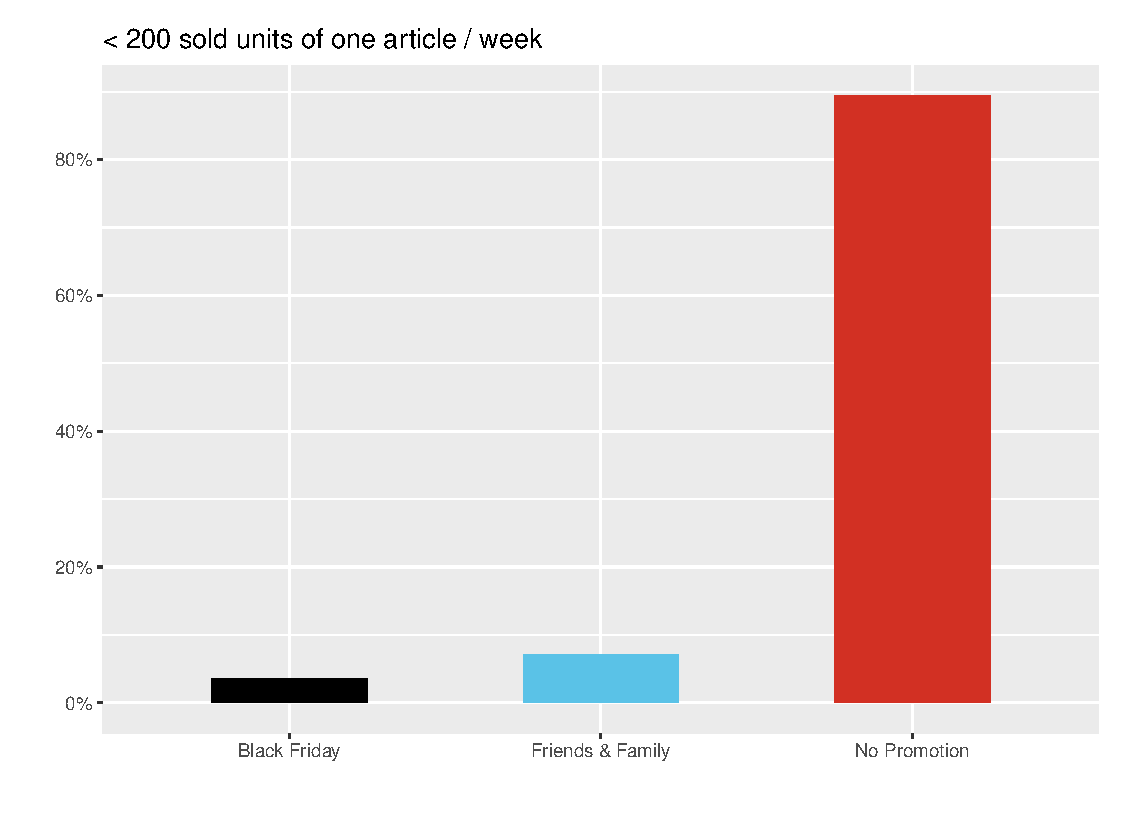
\includegraphics[width=\linewidth]{figures/bar_below_200_units_week.eps}
  \caption{Below 200 units}
  \label{fig:bar_below_200_units_week}
\end{subfigure}
\begin{subfigure}{.45\textwidth}
  \centering
  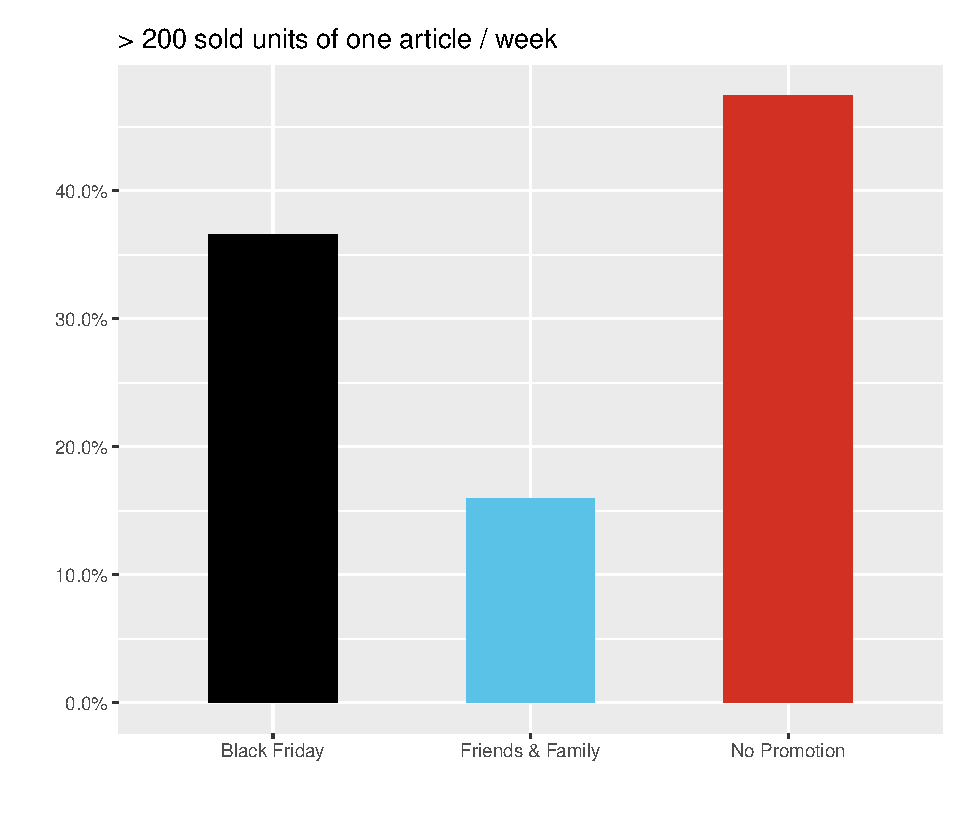
\includegraphics[width=\linewidth]{figures/bar_above_200_units_week.eps}
  \caption{Above 200 units}
  \label{fig:bar_above_200_units_week}
\end{subfigure}
\caption{Distribution of sold units of articles per week split at 200 units}
\label{fig:200_split_plots}
\end{figure}


To validate the exploration on this, we may look at the empirical \ac{CDF} in \autoref{fig:ecdf_all} using all observations now.
Instances with no promotions have a steeper curve (red line) and reach their maximum faster compared to articles tagged with a promotion in a certain week. The less concave curve of Friends \& Family promoted sales (blue line) implies that there are more instances with a larger amount of sold units overall. The same behaviour is even more pronounced for Black Friday (black line), having considerably more high quantity instances. Along these lines, promotions might somewhat explain this pattern better.\\
 
 
 \begin{figure}[H]
\centering
  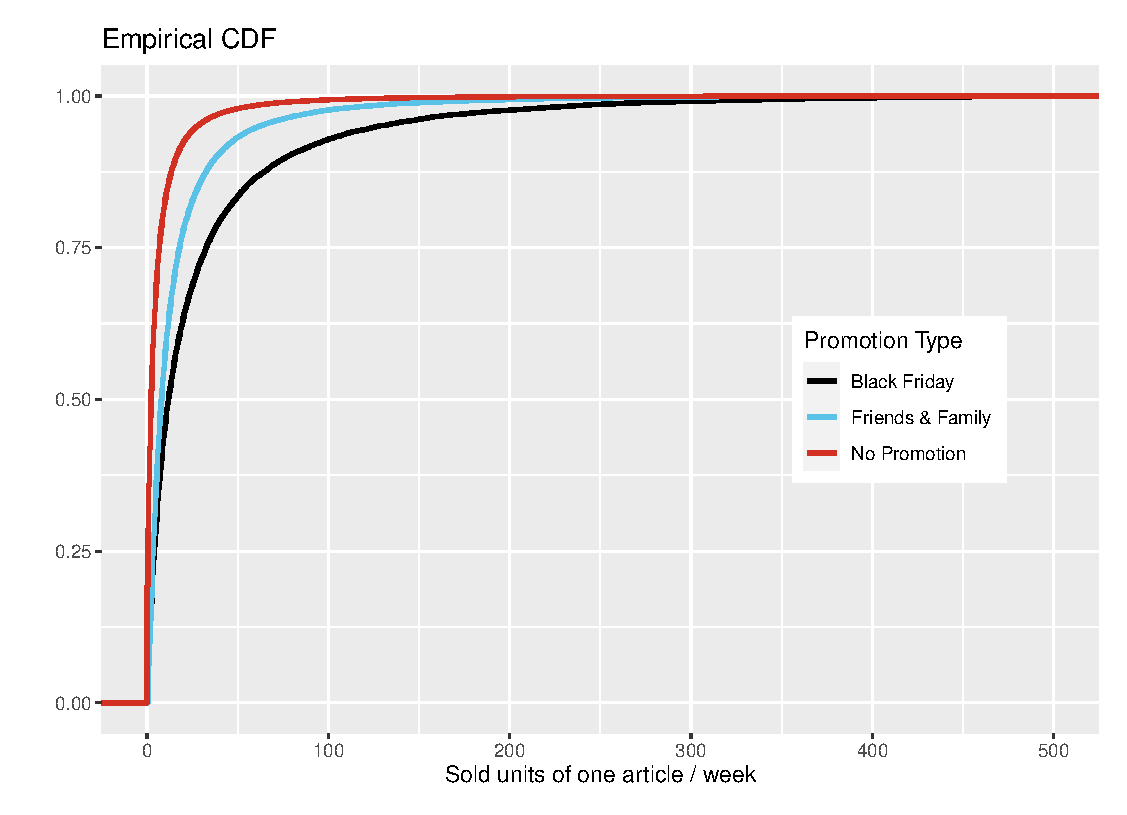
\includegraphics[width=0.65\linewidth]{figures/ecdf_all.eps}
  \caption{Empirical \ac{CDF} of all sold units per week; x-axis cut at 500}
  \label{fig:ecdf_all}
\end{figure}



Unfortunately, such outliers with extreme sale numbers should not be removed from the dataset, as it would produce gaps in the time series of some specific articles. Removing entire articles from the analysis is also not an option at this point, since we would be forced to remove a lot of articles.
%There will be a data delimitation process down the line to deal with this issue (see Subsection \ref{sssec:data_delimitation}). 
For example, 273 articles alone would have to be removed to get rid of the highest 0.01\% of quantities (see \autoref{tab:quantiles_sold_units_week}). Besides, these extreme values might be too informative for the underlying data generating process, so no removal of instances will be employed to the dataset.









\subsection{Grouped Sale Patterns - Key Category Cluster} \label{ssec:grouped_patterns}
% !TEX root = Master.tex


To gain some insights on a hierarchical level of interest, some quick analysis is performed on different groups (nodes) of the key category cluster level in the tree (see \autoref{fig:article_hierarchy}). We start out with a broad picture on this upper level 
%in Subsection \ref{sssec:kcc_exploration} 
and eventually reach a better understanding for the the article behaviour.
\\



By viewing the sale trends separately for each key category cluster, we can observe in \autoref{fig:ts_log_sales_kcc} that, among the weekly noise, they climax similarly. Just like in the previous section, those peaks come about primarily during the big promotions weeks. To put it into perspective, we can see logarithmic sale behaviour in \autoref{fig:boxplot_log_sales_kcc}, were patterns are quite similar although they differ strongly in volume. 
\\

 \begin{figure}[H]
\centering
\begin{subfigure}{.45\textwidth}
  \centering
  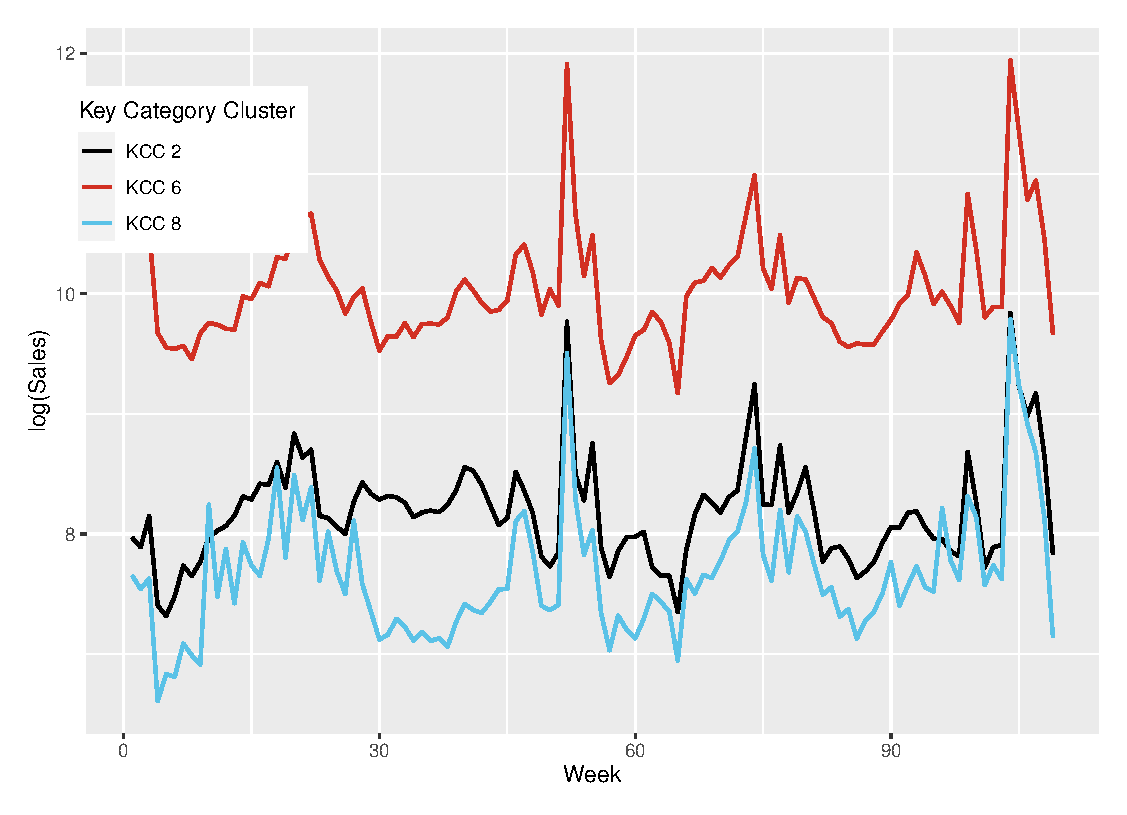
\includegraphics[width=\linewidth]{figures/ts_log_sales_kcc.eps}
  \caption{Time series of log(Sales) per KCC}
  \label{fig:ts_log_sales_kcc}
\end{subfigure}
\begin{subfigure}{.45\textwidth}
  \centering
  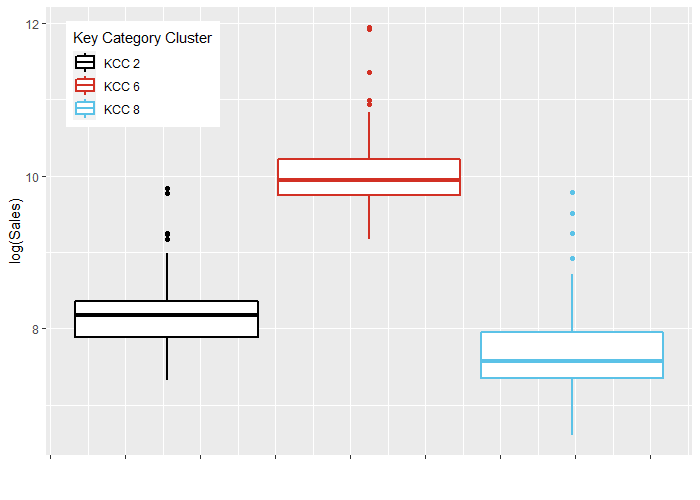
\includegraphics[width=\linewidth]{figures/boxplot_log_sales_kcc.png}
  \caption{Boxplots of log(Sales) per KCC}
  \label{fig:boxplot_log_sales_kcc}
\end{subfigure}
\caption{Time series and boxplot showing logarithmized sales of the key category clusters}
\label{fig:kcc_ts_and_boxplot}
\end{figure} 




\begin{figure}[H]
\centering
  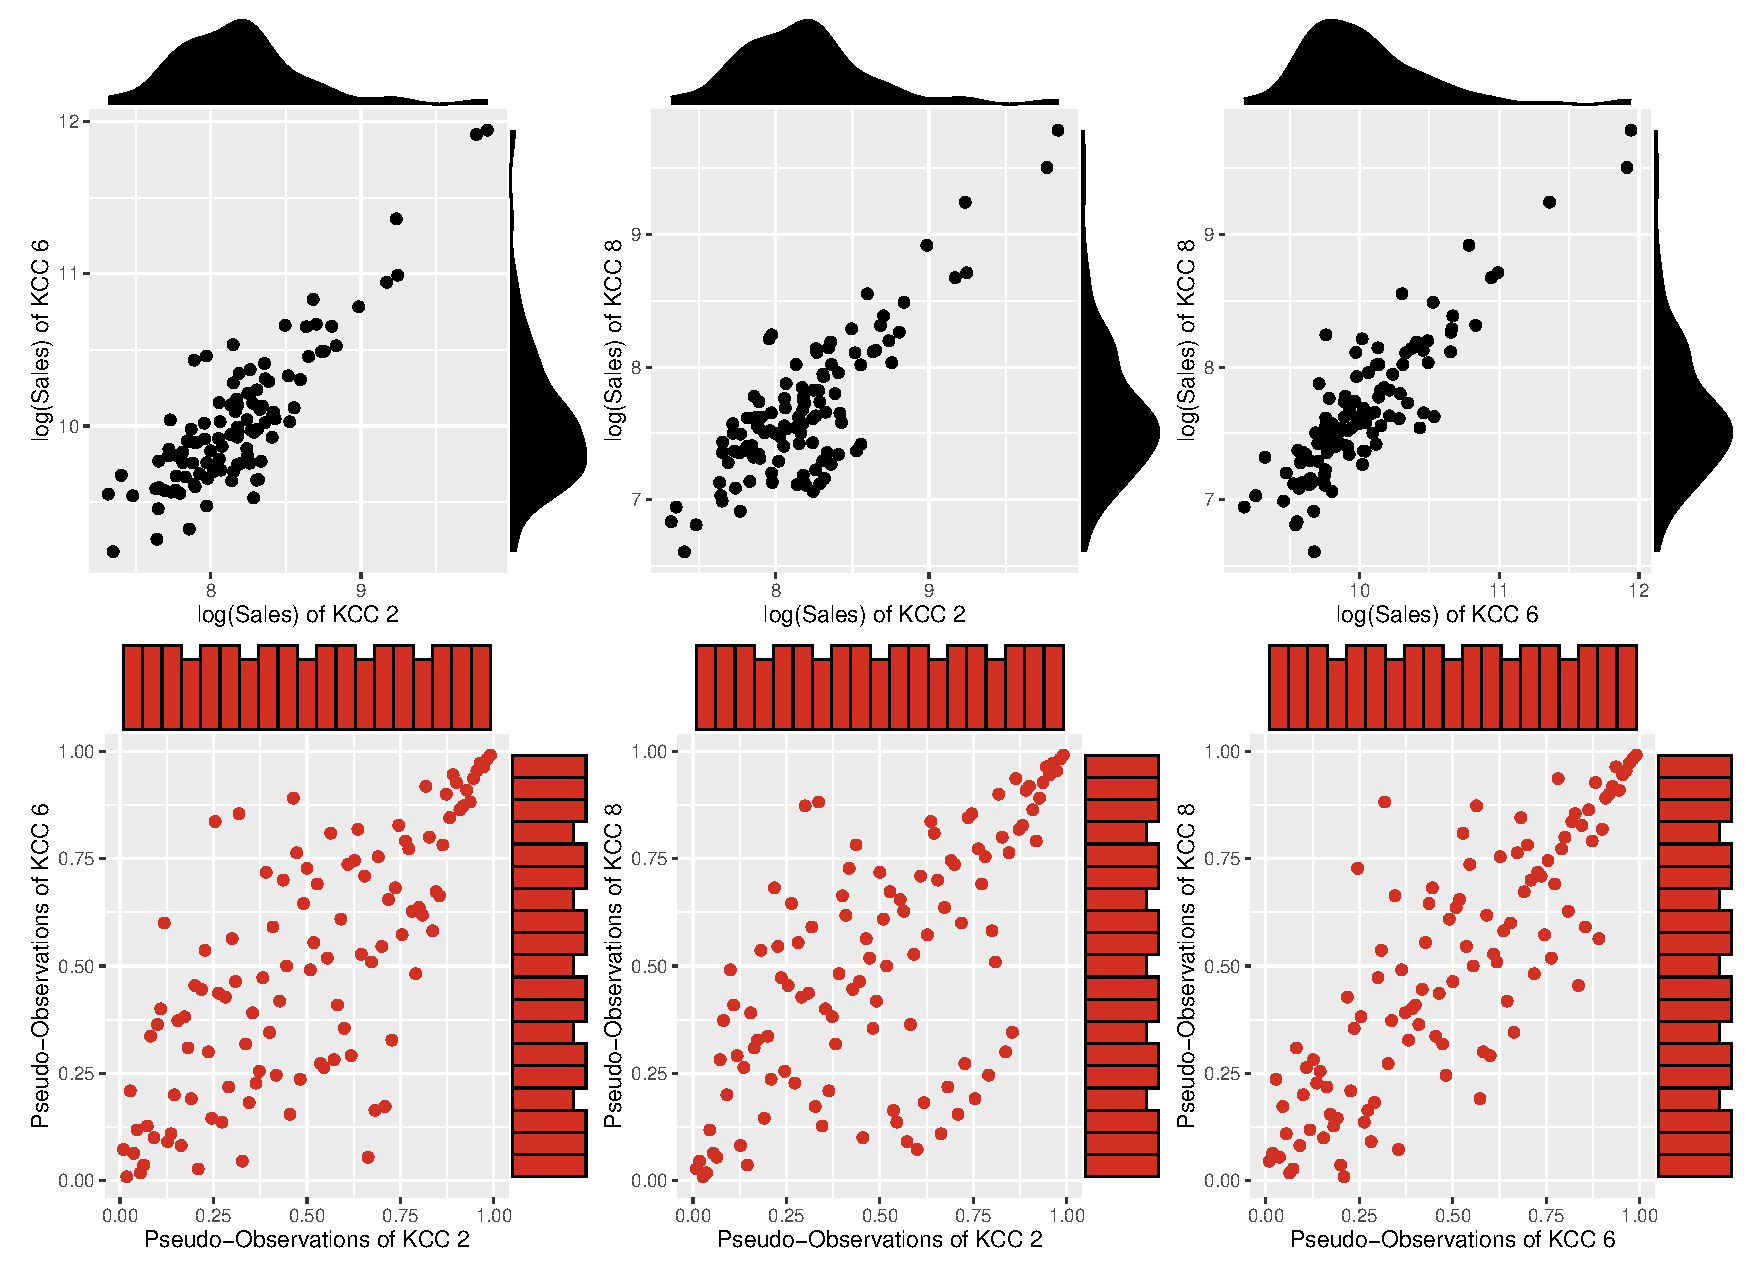
\includegraphics[width=0.95\linewidth]{figures/kcc_pair_scatterplots.eps}
  \caption{Pairwise scatterplots of sales on \ac{KCC} level. First row: Logarithmic sales with marginal densities, Second row: Pseudo sales observation with marginal histograms}
  \label{fig:kcc_pair_scatterplots}
\end{figure}


All the more interesting are the joint distributions of our \acp{KCC}. \autoref{fig:kcc_pair_scatterplots} shows scatterplots of \ac{KCC} pairs. In the first row we can see some isolated points on the upper tails representing outliers. We took the logarithmized sales to spot differences that would be otherwise hard to see. The outliers produced by the promotions still remain outliers in the log-scale. Also, by checking the densities for the marginals, pertinent marginal distributions are hardly determined but not to be ruled out.\\
The second row displays the pairs of the according \textit{pseudo observations}. Pseudo observations are calculated by taking the data ranks and dividing them by "1 + number of observations", which makes them robust against outliers and restricts the value range to $(0, 1)$. Here we are faced with a strange behaviour of the histograms. They practically look uniformly distributed, however there are seemingly regular step patterns in the pseudo data. This might be traced back to the fact that we are dealing in reality with discrete data of not necessarily unique occurrence.\\

For the above reasons, on \ac{KCC} level we will attempt modelling parametric distributions to the marginals (see Chapter \ref{sec:modelling}). 
%The reason being for the latter is that our primary objective is to capture a dependence structure, whereas the marginals per se are of secondary interest. 
In addition, looking at both rows of \autoref{fig:kcc_pair_scatterplots}, we suspect tail dependence and there is an obvious strong positive correlation among all three pairs, which is confirmed by viewing \autoref{fig:corplot_kcc} displaying various correlation metrics.
 \\


\begin{figure}[H]
\centering
  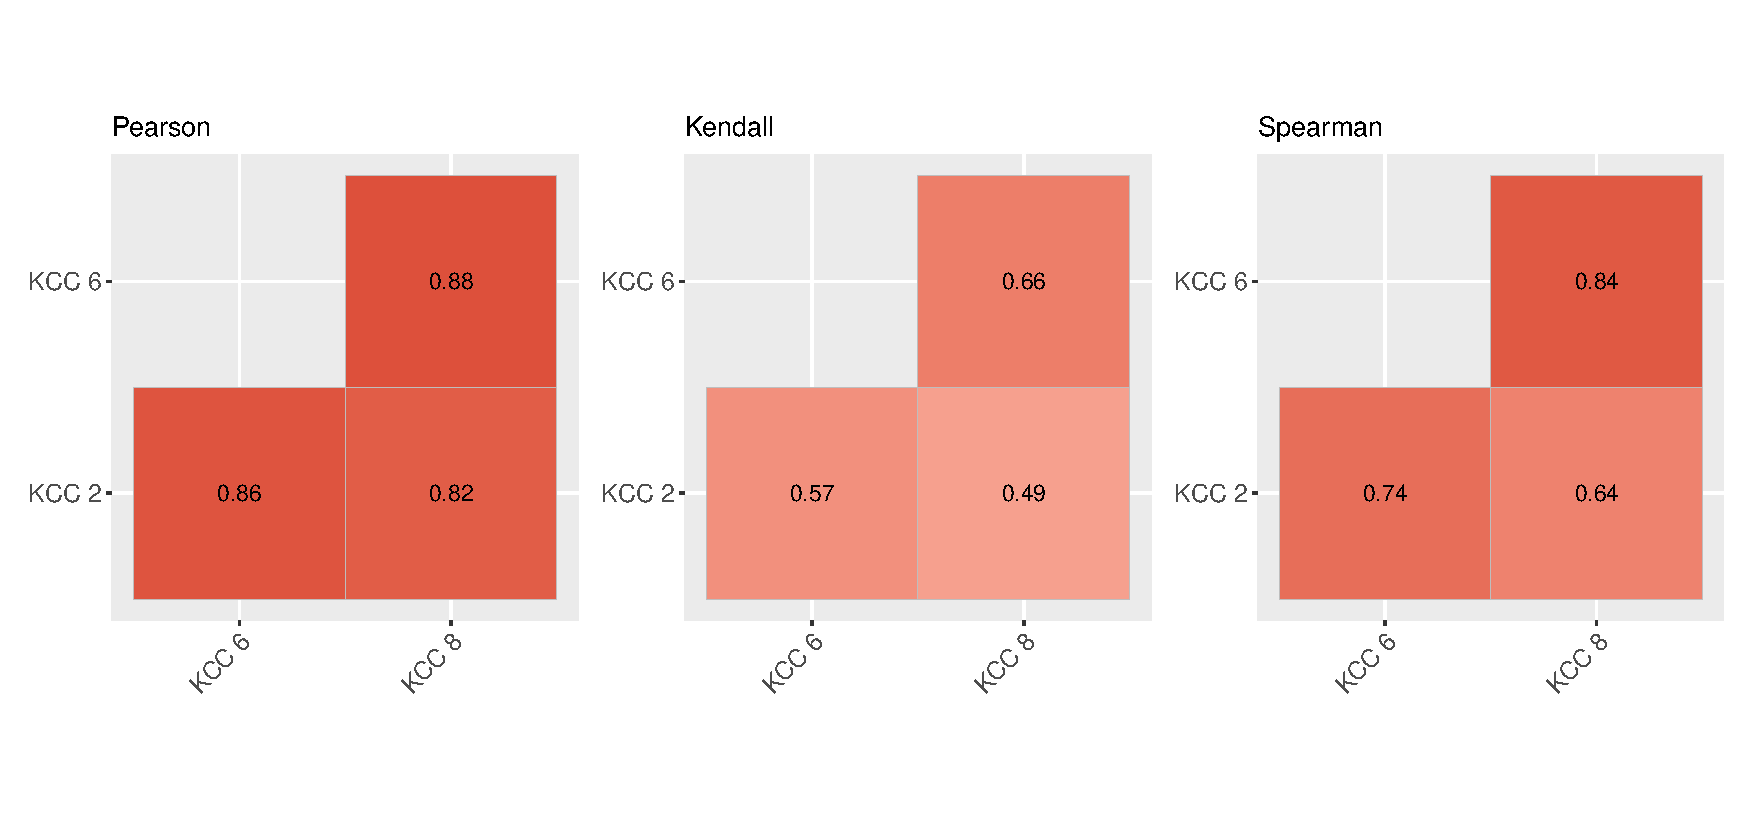
\includegraphics[width=0.95\linewidth]{figures/corplot_kcc.eps}
  \caption{Correlation plots of the three \ac{KCC} log-sales with different correlation coefficients. Left: Pearson's rho, Middle: Kendall's tau, Right: Spearman's rho}
  \label{fig:corplot_kcc}
\end{figure}




One side note on the promotion intensities of Black Friday and Friends \& Family (see \autoref{tab:transactional_data}) is that on higher levels such as key category cluster, as we aggregate our data, promotion intensities become binary values indicating whether the respective promotion took place in those respective weeks. Also note that Black Friday and Friends \& Family weeks do not overlap. The boxplots of the two promotion types depicted in \autoref{fig:bf_kcc_boxplot} and \autoref{fig:ff_kcc_boxplot} point out how they affect the sales. Though, one shall keep in mind that, out of 109 weeks, only the minority include promo activation. Precisely, Black Friday is activated over 6 weeks out of 109 and Friends \& Family is activated over 13 weeks\footnote{And of course not in a row, as can be clearly observed in \autoref{fig:total_sold_articles_ts}.} (see Tables \ref{tab:black_friday} and \ref{tab:friends_and_family}). In \autoref{fig:ff_kcc_boxplot}, one shall also be aware of large outliers being present during no Friends \& Family weeks, which is fairly aligned with what we figured out in the previous subsection (i.e. many sale occurrences do not have any promotion).
\\


\begin{figure}[H]
\centering
  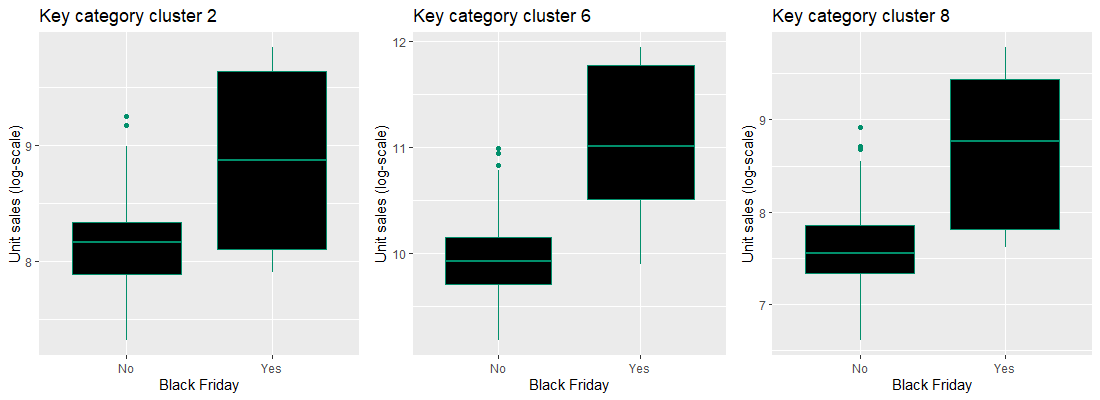
\includegraphics[width=0.95\linewidth]{figures/bf_kcc_boxplot.png}
  \caption{Boxplots showing log-sales of KCCs against presence of Black Friday}
  \label{fig:bf_kcc_boxplot}
\end{figure}


\begin{figure}[H]
\centering
  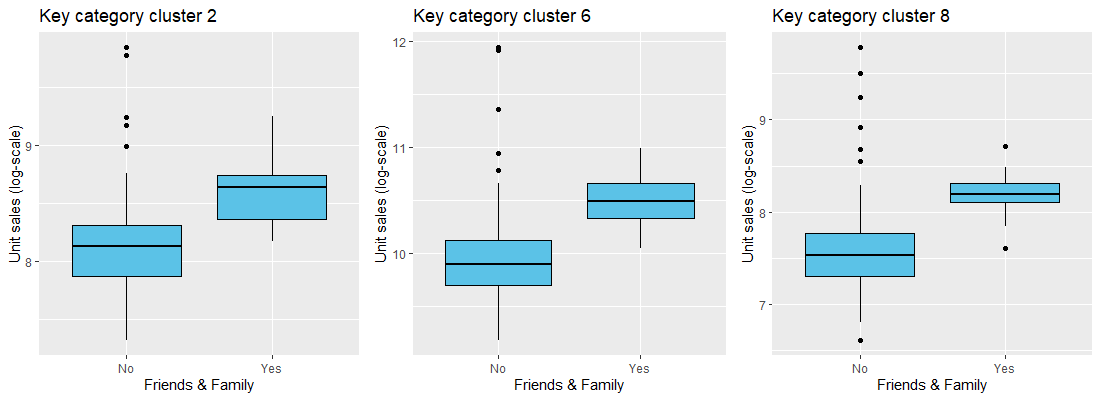
\includegraphics[width=0.95\linewidth]{figures/ff_kcc_boxplot.png}
  \caption{Boxplots showing log-sales of KCCs against presence of Friends \& Family}
  \label{fig:ff_kcc_boxplot}
\end{figure}


The scatterplots in \autoref{fig:total_markdown_against_kcc} clearly reveal the strong positive relationship between the log-sales and the \ac{KCC}s' respective total markdown percentages.
\\
Regarding the season type (SS vs FW), visual exploration is not sufficient to conclude existence of effects on the unit sales. The effect of season type as well as other features on the unit sales shall be discussed in Chapter \ref{sec:modelling}.
\\




\begin{figure}[H]
\centering
  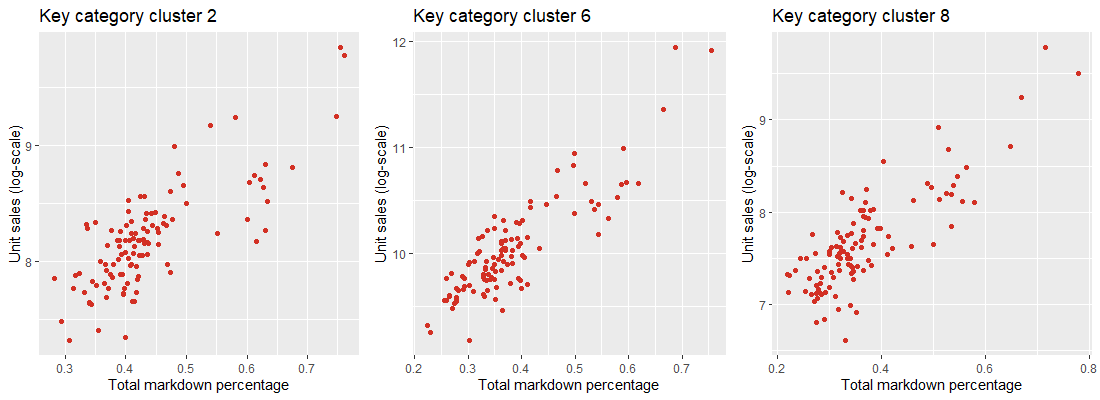
\includegraphics[width=0.95\linewidth]{figures/total_markdown_against_kcc.png}
  \caption{Scatterplots of \ac{KCC} log-sales against total markdown percentage}
  \label{fig:total_markdown_against_kcc}
\end{figure}






\begin{figure}[H]
\centering
  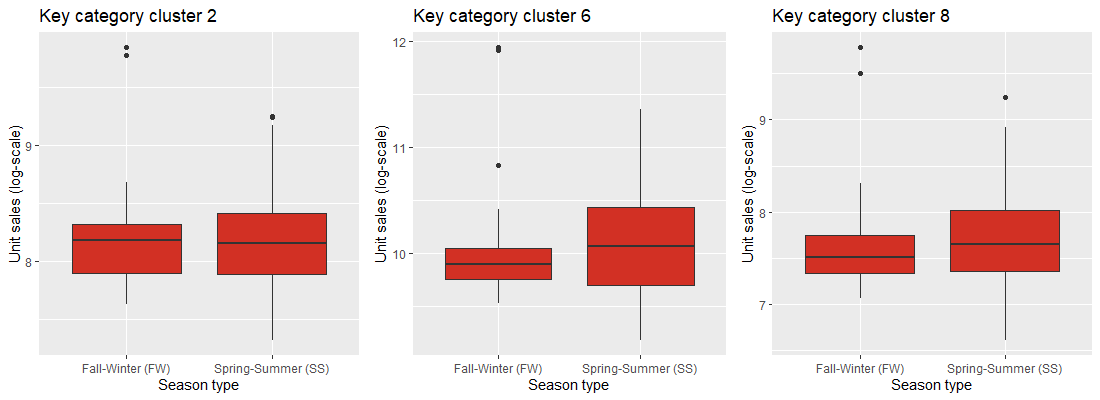
\includegraphics[width=0.95\linewidth]{figures/season_type_against_kcc.png}
  \caption{Boxplots of \ac{KCC} log-sales against the two season types}
  \label{fig:season_type_against_kcc}
\end{figure}






\subsection{Individual Sale Patterns} \label{ssec:individual_patterns}
% !TEX root = Master.tex


So far we explored the data pinpointing multiple characteristics of article unit sales along with other features in an aggregate or grouped frame. This section will briefly highlight some additional aspects of demand quantities regarding individual articles and the associated limitations.
\\

Straight away, the biggest challenge is the life cycle of the articles. A sample of seven articles will list some these challenges. The course of those article sales is plotted in \autoref{fig:article_sample}. Article "5040" for example has only a lifespan of a 18 weeks and there are 12,679 out of 26,203 distinct articles having even less than that, which is almost half of the dataset. There are thousands of articles which have a lifespan of single digit (in weeks). The barplot in \autoref{fig:article_lifespan} makes the extent of this issue visible. Articles that were observed during the entire observation window (or at least the majority of it) are the exception to the rule. It should be mentioned also that many articles started their selling journey on eCom before 2017 where the data for this task were acquired and other articles are still being in stock after 2018 (probably the case for article "21928"). These troublesome facts make it very hard to apply any kind of promising quantitative methods. Nevertheless, this issue will be discussed in later parts of this thesis (see Section \ref{ssec:article_dependencies}).
\\


\begin{figure}[H]
\centering
  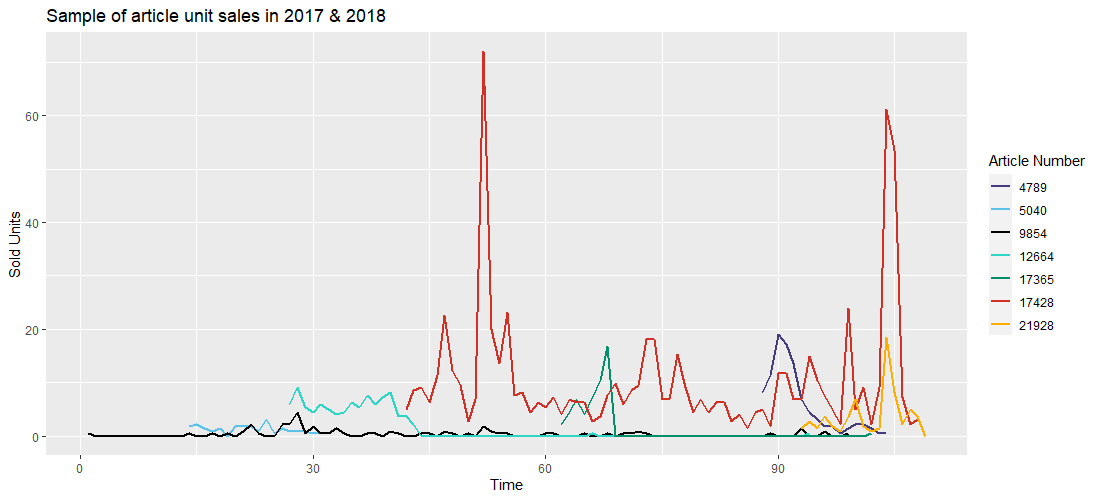
\includegraphics[width=0.95\linewidth]{figures/article_sample.png}
  \caption{Sample of seven articles and their demand quantity life cycles}
  \label{fig:article_sample}
\end{figure}


\begin{figure}[H]
\centering
  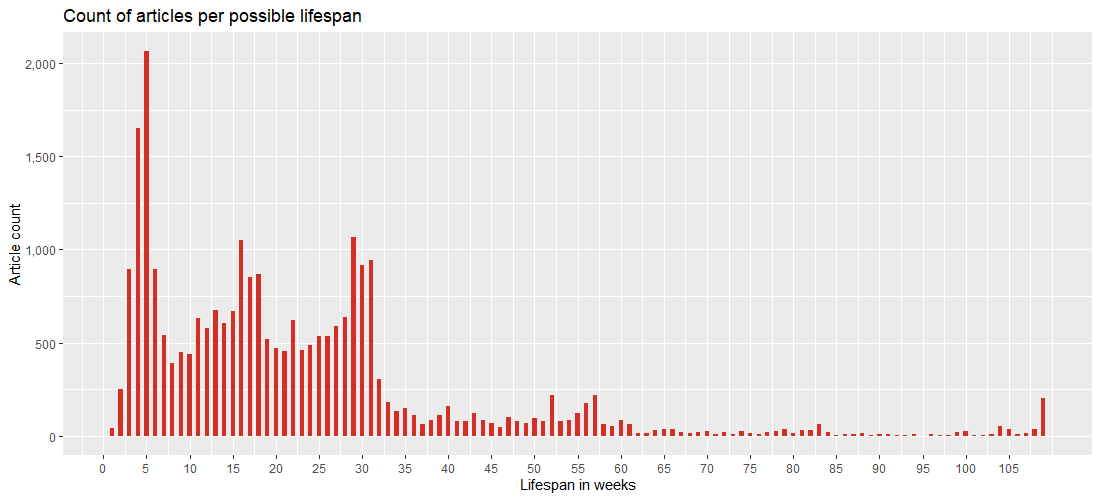
\includegraphics[width=0.95\linewidth]{figures/article_lifespan.png}
  \caption{Number of articles for each possible lifespan of 1 to 109 weeks}
  \label{fig:article_lifespan}
\end{figure}



Yet another immediate remark is the zero inflation persisting in the data. A lot of articles spend their time on eCom for several weeks without being sold once, as can be seen e.g. in \autoref{fig:article_sample} for articles "9854", "12664" and "17365". To be precise, for 100,732 instances we have a gross demand quantity of zero, which makes up almost a fifth of the dataset. Combining this inflation of zeros with the short lifespan increases the level difficulty even more.







\newpage
\thispagestyle{empty}
\cleardoublepage

\thispagestyle{plain}
\section{Modelling} \label{sec:modelling}
% !TEX root = Master.tex

In this chapter, we explore diverse ways on how to model, evaluate and interpret the dependence structure of unit sales. 
%We first start at key category cluster level and compare the capabilities of the tried and tested methods on article unit sales. 
\\


%When we aggregate our data, not only promotion intensities need to be adapted. In the course of this, we average the total markdown percentage of all articles belonging to a respective aggregation group, e.g. each key category cluster obtains its own mean total markdown percentage. However, when we are trying to model dependence measures of pairwise groups as functions of covariates, we need a unifying feature for those groups. Luckily, we can readily average the aggregated total markdown percentages. \autoref{fig:total_markdown_pct_kcc} clarifies the strong linear correlations of those aggregated markdown percentages, therefore this simple solution should be rational. \\


%\begin{figure}[H]
%\centering
 % 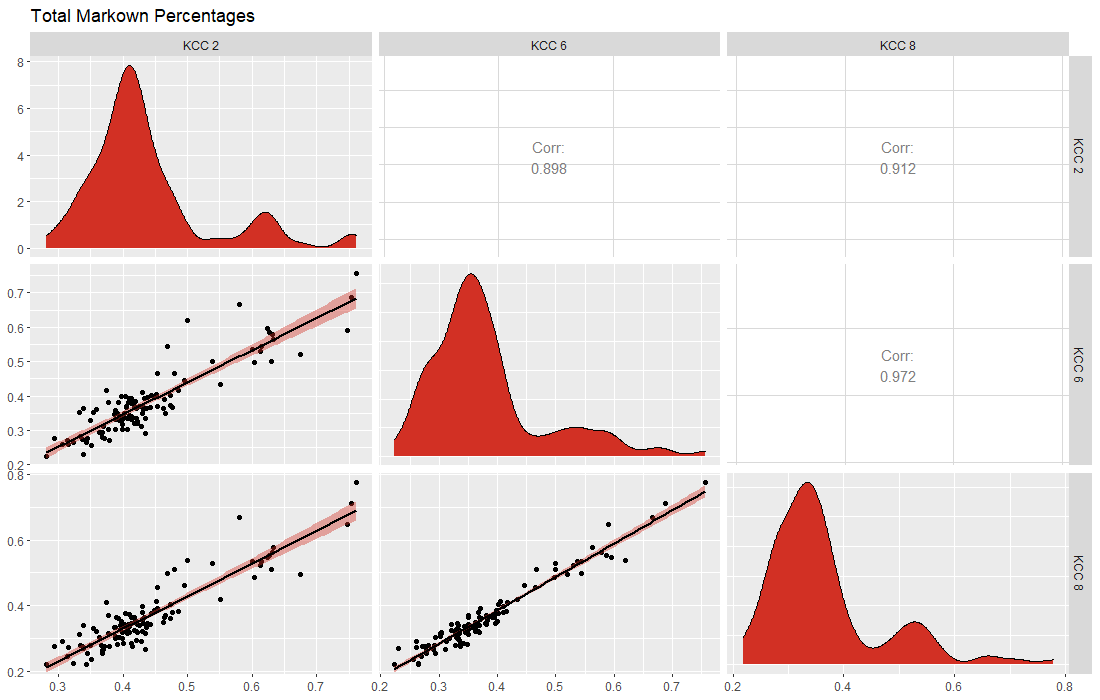
\includegraphics[width=0.8\linewidth]{figures/total_markdown_pct_kcc.png}
%  \caption{Pairwise total markdown percentages of key category clusters}
%  \label{fig:total_markdown_pct_kcc}
%\end{figure}

An important aspect of the modelling part is that usually, continuous responses are implied in the literature. Nevertheless, discrete responses (like in our "real" case) are also justified when explanatory variables are involved. A detailed explanation can be found in \cite{trivedi2017note}.\\ 
As the observation period is only 109 weeks and the highest peaks occur during Black Friday twice, the second time being very late (104th week, see e.g. \autoref{fig:total_sold_articles_ts}), all of the modelling is being performed in-sample. Thus, evaluation and diagnostics are based on the entire observation period so that both extreme peaks can be included in model trainings.\\
This chapter starts with Section \ref{ssec:kcc_margins}, where we fit the logarithmic sales (semi-)parametrically within the \ac{GAMLSS} framework. Next, in Section \ref{ssec:kcc_copulas}, we use a conditional copula approach using the residuals of Section \ref{ssec:kcc_margins} as responses in order to obtain correlation structures between the key category cluster pairs. In Section \ref{ssec:article_dependencies}, a short application of a dynamic Bayesian network is introduced and an outlook for further possible research is discussed. %Section \ref{ssec:discussion} contains a summarizing discussion about the chapter as well as an outlook for potential future research.



\subsection{Key Category Cluster - Marginal Distributions} \label{ssec:kcc_margins}
% !TEX root = Master.tex

\autoref{fig:kcc_pair_scatterplots} (Section \ref{ssec:grouped_patterns}) is hinting that the marginal distributions come with a noticeable skewness, which are best to take into account. The logarithmic scale is the preferred transformation due to variance stabilization of the margins. Among a pool of possible parametric distributions, we pick an appropriate one for each margin. Several distributions would theoretically be justifying the shape of our data, e.g. Weibull, Gamma, Box-Cox-Cole-Green or Dagum distribution. After screening those parametric distributions, we find that the exponentially modified Gaussian distribution (or ex-Gaussian distribution which is used from here on) fits all three margins fairly well \citep{grushka1972characterization}.\footnote{Another appropriate distribution would be the Dagum distribution \citep{dagum1975model}, however interpretability of the parameters is difficult to comprehend.} 
%Although the distribution assumptions are aligned with the empirical distributions of the data, there are still some expected outliers. This is quite visible in Figures \ref{fig:kcc_2_margin} to \ref{fig:kcc_8_margin}, which depict the marginal empirical distributions along with the theoretical assumptions, especially when looking at the Quantile-Quantile Plots (right figures).
Before entering the dependence structures between the three \ac{KCC} pairs, the marginal distribution of each cluster is analyzed individually in the next three subsections. First, the ex-Gaussian distribution is fitted to the margins and in a second step covariate effects are included to obtain flexible estimations on the distribution parameters.
%\footnote{Maximum likelihood estimation of a simple \ac{GAMLSS} model (see \cite{rigby2005generalized}).} 




%For the approaches in the below Section \ref{ssec:kcc_correlations} requiring parametric distribution assumptions for the margins, we will consider the Dagum distribution with parameters specified as in the captions of the above three figures, which represent estimated maximum likelihood values (that is, if they do not have to be estimated over again within a model like e.g. \ac{GAMLSS}).




\subsubsection{Key Category Cluster 2} \label{sssec:margin_kcc_2}
% !TEX root = Master.tex

Simple maximum likelihood estimation based on the log-sales of the marginals allow us to estimate the exGaussian distribution parameters. \autoref{fig:kcc_2_density} describes how the histogram of the data match to the theoretical density of an exGaussian distribution considering the estimated parameter values represented in \autoref{tab:estimated_parameters_kcc_2_no_covariates}.
\\




\begin{table}[H]
\setlength\arrayrulewidth{1pt}  
\centering
\begin{adjustbox}{max width=\textwidth}\
\begin{tabular}{|c|c|c|}
\hline
\rowcolor{lightgray} 
$\hat{\mu}$ & $\hat{\sigma}$ & $\hat{\nu}$ \\ \hline
7.85        & 0.26           & 0.33        \\ \hline
\end{tabular}
\end{adjustbox}
\caption{Estimated parameters for log-sales of KCC 2 fitted to exGaussian distribution with no covariate effects}
\label{tab:estimated_parameters_kcc_2_no_covariates}
\end{table}





 \begin{figure}[H]
\centering
\begin{subfigure}{.45\textwidth}
  \centering
  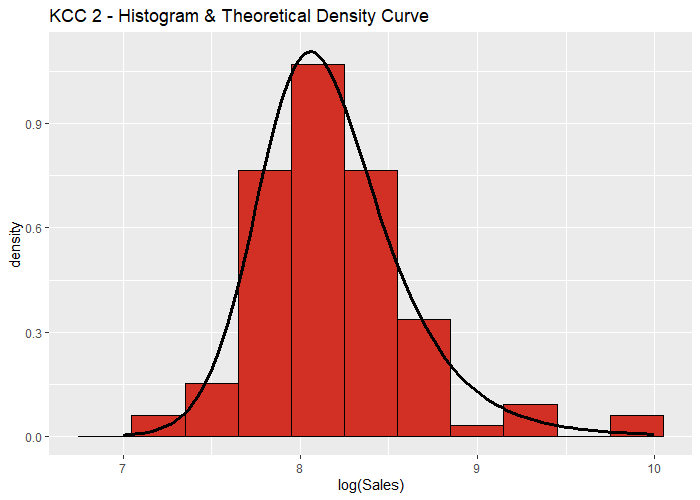
\includegraphics[width=\linewidth]{figures/kcc_2_density.png}
  \caption{Histogram \& theoretical density}
  \label{fig:kcc_2_density}
\end{subfigure}
\begin{subfigure}{.45\textwidth}
  \centering
  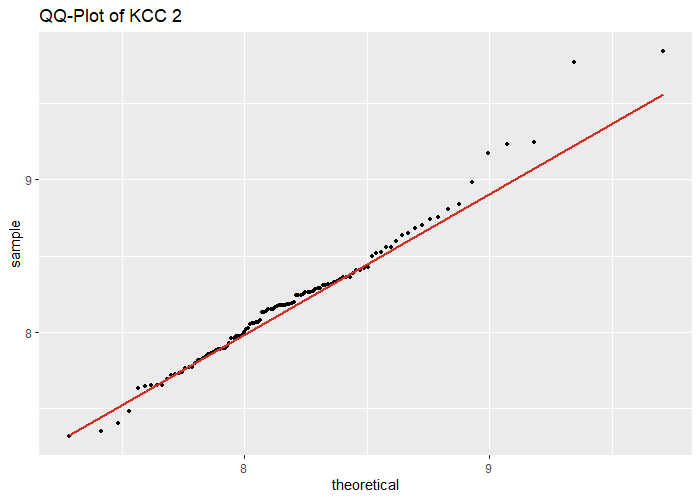
\includegraphics[width=\linewidth]{figures/kcc_2_qqplot.png}
  \caption{QQ-Plot}
  \label{fig:kcc_2_qqplot}
\end{subfigure}
\caption{exGaussian distribution fitted to log-sales of \ac{KCC} 2}
\label{fig:kcc_2_marginal}
\end{figure} 




\begin{figure}[H]
\centering
  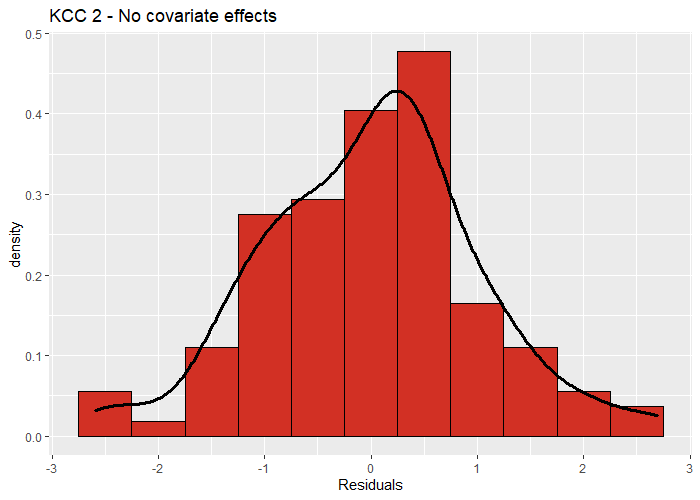
\includegraphics[width=0.45\linewidth]{figures/res_kcc_2_no_covariates.png}
  \caption{Residuals of KCC 2 log-sales fitted to an exGaussian distribution with no covariate effects together with their density curve}
  \label{fig:res_kcc_2_no_covariates}
\end{figure}

As can be seen in \autoref{fig:res_kcc_2_no_covariates}, the residuals of the fitted distribution are not too far from a normal distribution. 
In fact, a Shapiro-Wilk normality test (see Section \ref{ssec:shapiro_wilk}) will fail to reject the null hypothesis, returning a p-value of 0.6645.
There still exist skewness in the distribution of the residuals and correction will be attempted in the following. \\

The findings so far indicate that the overall fit for this cluster is quite satisfiable and also supports interpretability of the estimated parameters. \\
To make the estimation more precise and to get a better understanding of what is driving sales, flexible estimation of the distribution parameters is required and thus covariate effects shall be included. \\
%The temporal effects in particular are of special interest. 

After multiple equation setups for the marginal distribution of \ac{KCC} 2, the chosen \ac{GAMLSS} model specification (see Section \ref{ssec:gamlss}) is as follows:

\begin{equation}
\begin{aligned}
\mu &= \beta_{01} + f_{11}(\textit{time}) + f_{12}(\textit{total\_markdown\_pct}) \\ \noalign{\vskip5pt}
log(\sigma) &= \beta_{02} + f_{21}(\textit{time}) \\ \noalign{\vskip5pt}
log(\nu) &=  \beta_{03}, 
\end{aligned}
\label{eq:gamlss_kcc_2}
\end{equation} \\
where the smooth functions $f_{11}$, $f_{21}$ and $f_{12}$ are build upon P-Splines with 20 knots each. For the scale and shape parameters ($\sigma$ and $\nu$ respectively) the logarithmic link function is used to ensure that they are mapped to the real positive line as the exGaussian distribution family can only capture positive skewness ($\nu$). For $\sigma$ we just use time as the only regressor and we set the skewness $\nu$ as a constant. The estimated location and scale parameters over time are depicted in \autoref{fig:gamlss_kcc_2_estimated_parameters} and in \autoref{tab:nu_ci_kcc_2} the estimated skewness parameter value with its 95\% confidence interval is shown. The scale parameter has an overall increasing trend within this data spectrum and the skewness parameter is closer to zero than in the maximum likelihood approach without any covariate effects.
\\


\begin{figure}[H]
\centering
  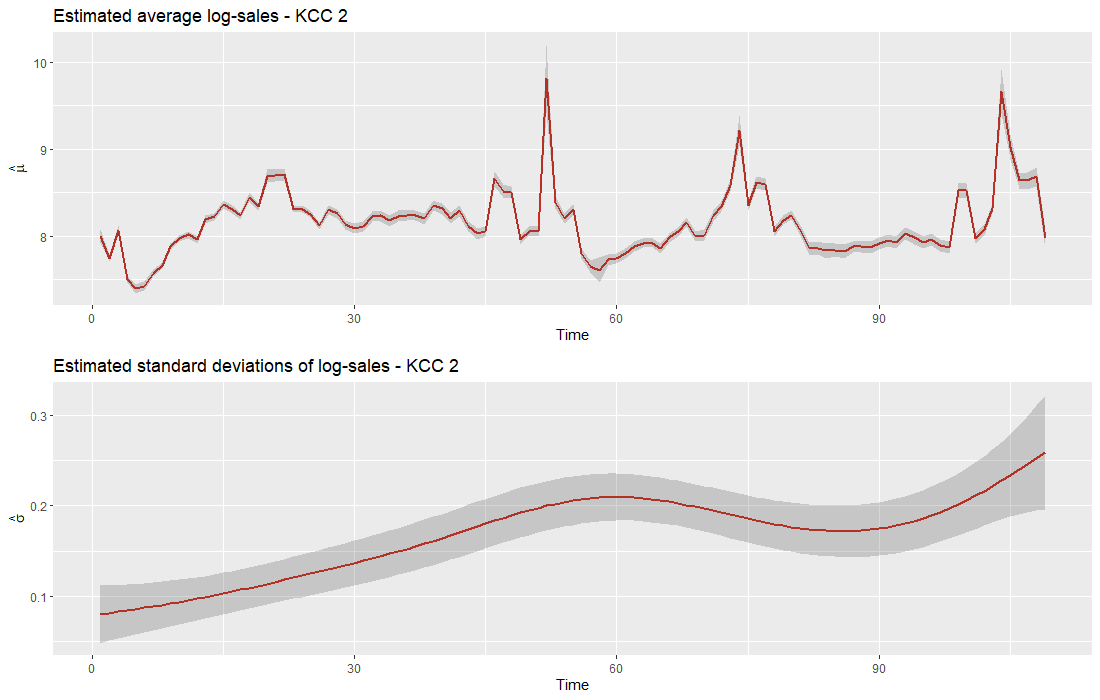
\includegraphics[width=0.95\linewidth]{figures/gamlss_kcc_2_estimated_parameters.png}
  \caption{Estimated location parameter $\hat{\mu}$ and scale parameter $\hat{\sigma}$ with confidence bands of GAMLSS fit - KCC 2}
  \label{fig:gamlss_kcc_2_estimated_parameters}
\end{figure}





\begin{table}[H]
\setlength\arrayrulewidth{1pt}  
\centering
\begin{adjustbox}{max width=\textwidth}\
\begin{tabular}{|c|c|c|}
\hline
\rowcolor{lightgray} 
Lower & $\hat{\nu}$ & Upper \\ \hline
0.007        & 0.021           & 0.037        \\ \hline
\end{tabular}
\end{adjustbox}
\caption{Estimated skewness parameter $\hat{\nu}$ of GAMLSS fit with 95\% confidence interval bounds - KCC 2}
\label{tab:nu_ci_kcc_2}
\end{table}



The absence of the Black Friday and Friends \& Family components in Model \ref{eq:gamlss_kcc_2} is due to the fact that the effects of activated promotions to the expected sales are negative, which is contradictory to the analysis made earlier in Chapter \ref{ssec:grouped_patterns}. The output after excluding those indicator variables seem to be more stable and is also more intuitive.\footnote{This might be traced back to the fact that promos obviously yield higher markdowns and thus we reach redundancy of variables in the model.} Below we can observe the summary output from the R console as well as the visual covariate effects on the expected value (\autoref{fig:gamlss_effects_kcc_2}).
\\



\VerbatimInput[frame = single, label = "GAMLSS Fit on KCC 2" ]{gamlss_fit_kcc_2_try20.txt}



From the visual representation of the covariate effects in (\autoref{fig:gamlss_effects_kcc_2}, we can see that until about August of 2017 (just below the 40th time observation) the log-sales are increasing and then from November on (roughly 50th observation) the log-sales remain at a constant level with somewhat higher values end of May (just below 80th observation). The overall course of the temporal effect on the response resembles a flat wavy line around zero, which is quite aligned with the coefficient in the R-output. Higher total markdown percentages enhance higher response values, which can also be observed when looking at the R-output. The estimated coefficient for the markdown obtains a value of 3.17. The seasonal effect of Spring-Summer is slightly lower than the effect of Fall-Winter. 
%The estimated standard error $\hat{\sigma}$ is generally increasing over time in this data spectrum (\autoref{fig:sigma_effect_kcc_2}). 
\\



\begin{figure}[H]
\centering
  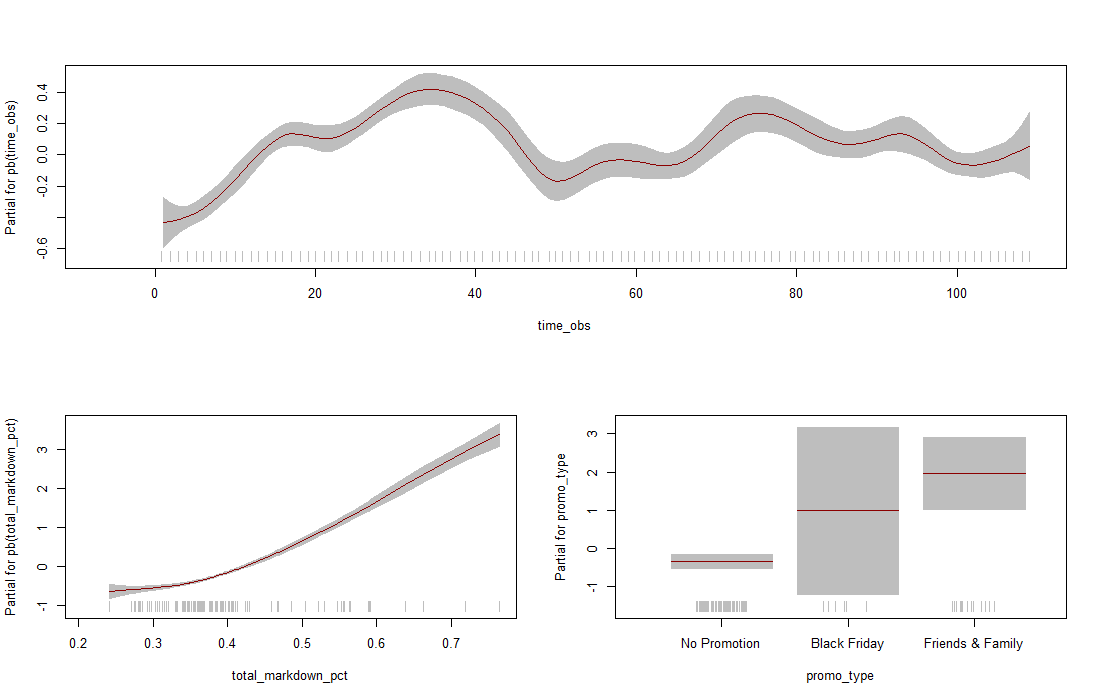
\includegraphics[width=0.95\linewidth]{figures/gamlss_effects_kcc_2.png}
  \caption{Covariate effects on the expected response variable (log-sales) of GAMLSS fit - KCC 2}
  \label{fig:gamlss_effects_kcc_2}
\end{figure}



%\begin{figure}[H]
%\centering
%  \includegraphics[width=0.95\linewidth]{figures/%sigma_effect_kcc_2.png}
%  \caption{Temporal effect on the scale parameter $%\hat{\sigma}$ - KCC 2}
%  \label{fig:sigma_effect_kcc_2}
%\end{figure}



Fitting the data to a \ac{GAMLSS} model like this can be considered favourable. The emerged residuals are closer to a standard normal distribution than the maximum likelihood estimation without any covariate effects. Diagnostic plots of quantile residuals in \autoref{fig:gamlss_residuals_kcc_2} confirm this. The R-output below \autoref{fig:gamlss_residuals_kcc_2} returns a detailed summary of the estimated location, scale and shape parameters of the residuals' distribution.
\\




\begin{figure}[H]
\centering
  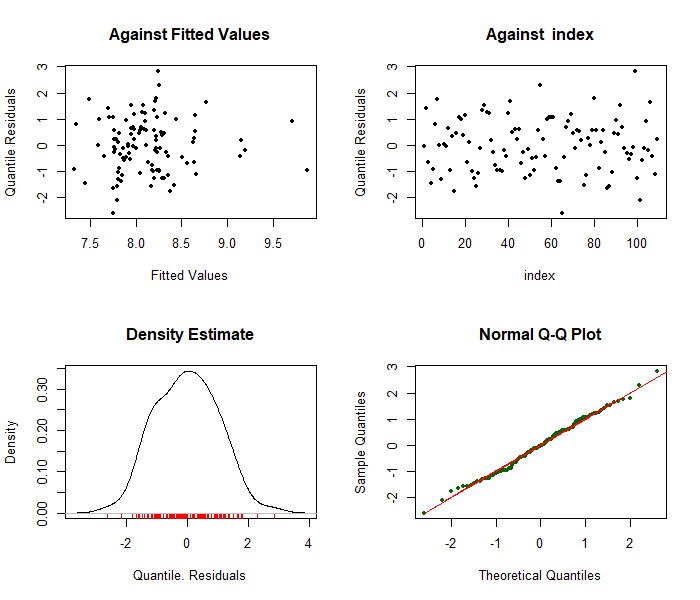
\includegraphics[width=0.95\linewidth]{figures/gamlss_residuals_kcc_2.png}
  \caption{Residuals of GAMLSS fit - KCC 2}
  \label{fig:gamlss_residuals_kcc_2}
\end{figure}




\VerbatimInput[frame = single, label = "Residuals of GAMLSS Fit on KCC 2" ]{gamlss_residuals_kcc_2.txt}



\subsubsection{Key Category Cluster 6} \label{sssec:margin_kcc_6}
% !TEX root = Master.tex

The same procedure as in Subsection \ref{sssec:margin_kcc_6} for key category cluster 2 is applied here to analyze the marginal distribution of the log-sales in key category cluster 6.\\

Excluding all covariates, simple maximum likelihood estimation results in parameters $\hat{\mu} = 9.62$, $\hat{\sigma} = 0.20$ and $\hat{\nu} = 0.41$ of the ex-Gaussian distribution.
\autoref{fig:kcc_6_density} shows the histogram of the observed log-sales along with a density curve fitted with the estimated parameters. A QQ-plot is displayed in \autoref{fig:kcc_6_qqplot}, where the data points match the line $y=x$ well, excluding a few outliers on the upper part of the plot.
 %can be summarized within \autoref{tab:estimated_parameters_kcc_6_no_covariates}, \autoref{fig:kcc_6_margin} and \autoref{fig:res_kcc_6_no_covariates}. 
 A Shapiro-Wilk test on the residuals returns a p-value of 0.87 and thus fails to reject the null hypothesis of non-normality. \autoref{fig:res_kcc_6_no_covariates} portrays a histogram of the residuals along with a density curve. Although it looks platykurtic to a certain extend, normality cannot be excluded as the Shapiro-Wilk test indicated.
\\


%
%\begin{table}[H]
%\setlength\arrayrulewidth{1pt}  
%\centering
%\begin{adjustbox}{max width=\textwidth}\
%\begin{tabular}{|c|c|c|}
%\hline
%\rowcolor{lightgray} 
%$\hat{\mu}$ & $\hat{\sigma}$ & $\hat{\nu}$ \\ \hline
%9.62        & 0.20           & 0.41        \\ \hline
%\end{tabular}
%\end{adjustbox}
%\caption{Estimated parameters for log-sales of KCC 6 fitted to ex-Gaussian distribution with no covariate effects}
%\label{tab:estimated_parameters_kcc_6_no_covariates}
%\end{table}



 \begin{figure}[H]
\centering
\begin{subfigure}{.45\textwidth}
  \centering
  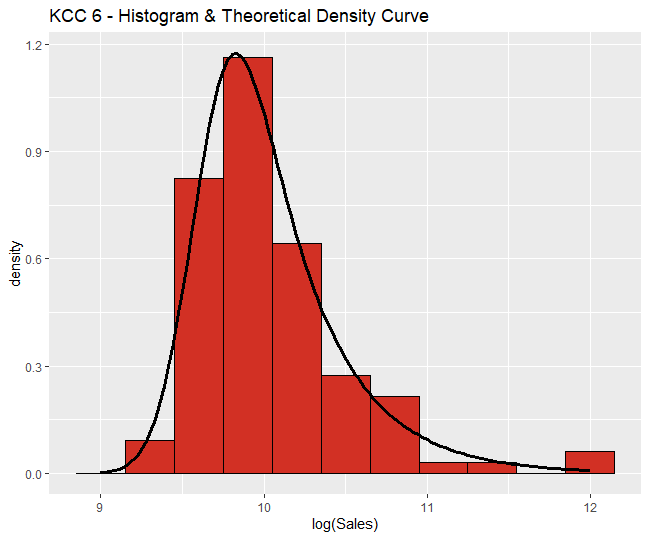
\includegraphics[width=\linewidth]{figures/kcc_6_density.png}
  \caption{Histogram \& theoretical density}
  \label{fig:kcc_6_density}
\end{subfigure}
\begin{subfigure}{.45\textwidth}
  \centering
  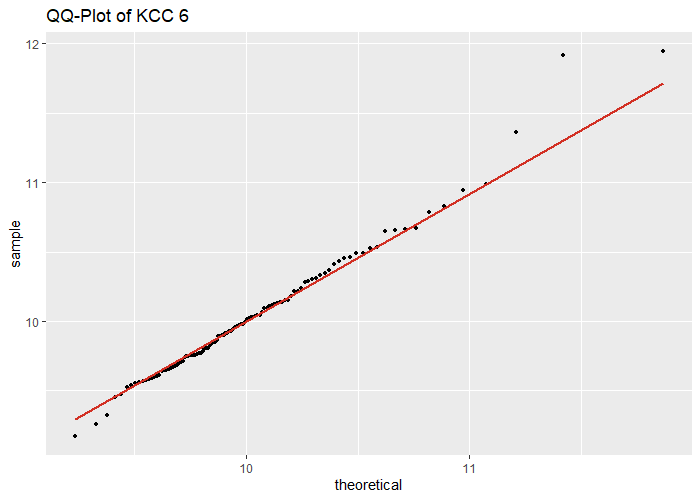
\includegraphics[width=\linewidth]{figures/kcc_6_qqplot.png}
  \caption{QQ-plot}
  \label{fig:kcc_6_qqplot}
\end{subfigure}
\caption{ex-Gaussian distribution fitted to log-sales of \ac{KCC} 6}
\label{fig:kcc_6_margin}
\end{figure} 


\begin{figure}[H]
\centering
  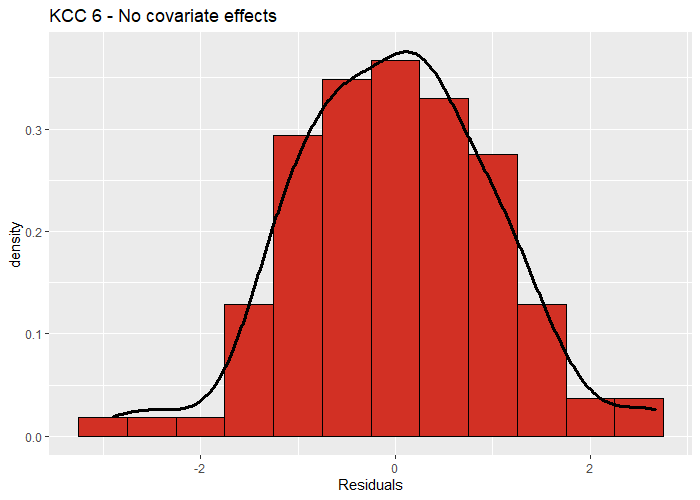
\includegraphics[width=0.45\linewidth]{figures/res_kcc_6_no_covariates.png}
  \caption{Residuals of KCC 6 log-sales fitted to an ex-Gaussian distribution with no covariate effects together with their density curve}
  \label{fig:res_kcc_6_no_covariates}
\end{figure}


Reviewing different model specifications, an equivalent model as in the previous Subsection is chosen (Model \ref{eq:gamlss_kcc_2}) with an ex-Gaussian distribution family for the response variable. The resulting parameter coefficients for $\hat{\mu}$ are printed in \autoref{tab:gamlss_coeff_kcc_6}, where we once again observe controversial results. A detailed summary of the model fit can be found in the \nameref{sec:appendix} (R output \ref{output:gamlss_fit_kcc_6_try1}). The two promotions seem to negatively interact with the total markdown percentage. Those kinds of behaviour might need further investigation.
The estimated time-varying location and scale parameters can be seen in \autoref{fig:gamlss_kcc_6_estimated_parameters} and the skewness parameter $\hat{\nu}$ with 95\% CI in \autoref{tab:nu_ci_kcc_6}. Fitted values are close to real values, capturing the promotion peaks fairly well. The standard deviation fluctuates throughout time within a range between 0.1 and 0.3.
\\


%\VerbatimInput[frame = single, label = "GAMLSS Fit on KCC 6" ]{gamlss_fit_kcc_6_try1.txt}



\begin{table}[H]
\centering
\begin{tabular}{l|c|c|c|l}
  \hline
  \rowcolor{white}
 \textbf{$\hat{\mu}$ Coefficients} & \textbf{Estimate} & \textbf{Std. Error} & \textbf{t value} & \textbf{p-value} \\ 
  \hline\hline
\textit{$\beta_{01}$ (Intercept)} & 8.31 & 0.11 & 71.80 & 0.00 *** \\ 
  \textit{$f_{11}$(time)} & 0.00 & 0.00 & 5.20 & 0.00 *** \\ 
  \textit{$f_{12}$(total\_markdown\_pct)} & 4.01 & 0.30 & 13.29 & 0.00 *** \\ 
  \textit{promo\_typeBlack Friday} & -0.81 & 0.30 & -2.73 & 0.01 ** \\ 
  \textit{promo\_typeFriends \& Family} & 0.87 & 0.48 & 1.81 & 0.07 . \\ 
  \textit{promo\_typeBlack Friday:total\_markdown\_pct} & 1.02 & 0.54 & 1.90 & 0.06 . \\ 
  \textit{promo\_typeFriends \& Family:total\_markdown\_pct} & -2.47 & 0.88 & -2.81 & 0.01 ** \\ \hline
\end{tabular}
\caption{Estimated $\hat{\mu}$ coefficients of \ac{GAMLSS} fit on log-sales of \ac{KCC} 6}
\label{tab:gamlss_coeff_kcc_6}
\end{table}





\begin{figure}[H]
\centering
  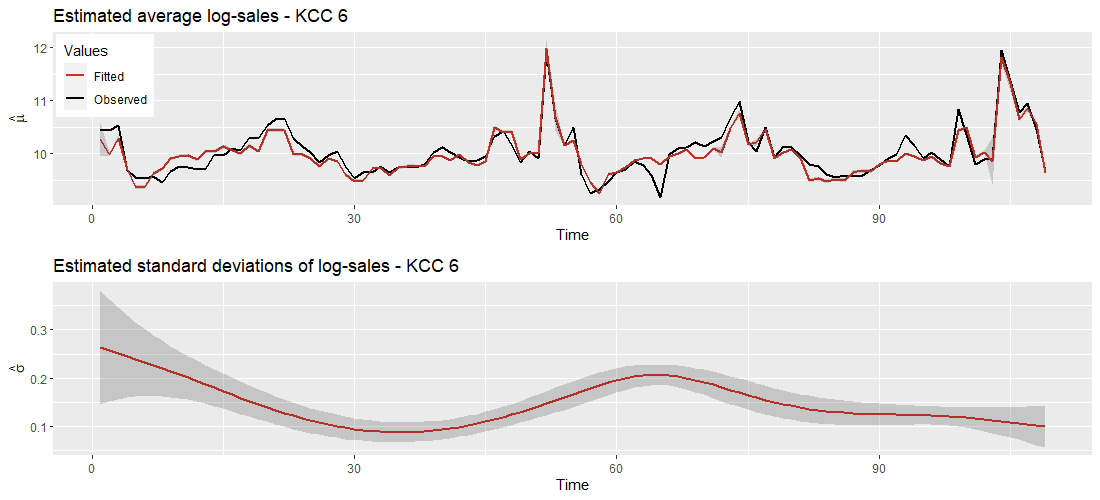
\includegraphics[width=0.95\linewidth]{figures/gamlss_kcc_6_estimated_parameters.png}
  \caption{Estimated location parameter $\hat{\mu}$ compared to the observed values and scale parameter $\hat{\sigma}$ with confidence bands of GAMLSS fit - KCC 6}
  \label{fig:gamlss_kcc_6_estimated_parameters}
\end{figure}



\begin{table}[H]
\setlength\arrayrulewidth{1pt}  
\centering
\begin{adjustbox}{max width=\textwidth}\
\begin{tabular}{c|c|c}
\hline
\rowcolor{white} 
\textbf{Lower} & $\hat{\nu}$ & \textbf{Upper} \\ \hline\hline
0.044        & 0.031           & 0.057        \\ \hline
\end{tabular}
\end{adjustbox}
\caption{Estimated skewness parameter $\hat{\nu}$ of GAMLSS fit with 95\% confidence interval bounds - KCC 6}
\label{tab:nu_ci_kcc_6}
\end{table}




\autoref{fig:gamlss_effects_kcc_6} reveals some interesting points regarding covariate effects. The temporal effect as well as the total markdown percentage collapse to increasing straight lines. 
%The temporal effect also exhibits symmetrical behaviour around zero, including uncertainty. 
%Just like in \ac{KCC} 2, the effect of Spring-Summer is slightly smaller than that of Fall-Winter.
As opposed to the \ac{GAMLSS} fit for \ac{KCC} 2, Friends \& Family seems to have the highest effect of all promos for this \ac{KCC}. 
\\



\begin{figure}[H]
\centering
  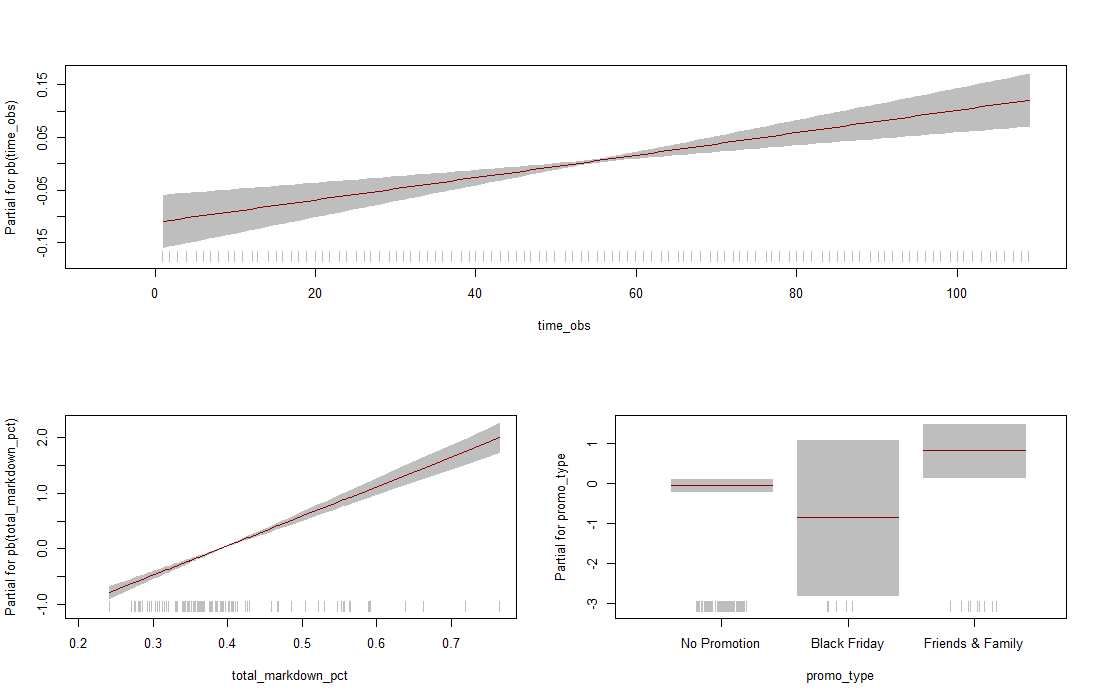
\includegraphics[width=0.95\linewidth]{figures/gamlss_effects_kcc_6.png}
  \caption{Covariate effects on the expected response variable (log-sales) of GAMLSS fit - KCC 6}
  \label{fig:gamlss_effects_kcc_6}
\end{figure}









\begin{figure}[H]
\centering
  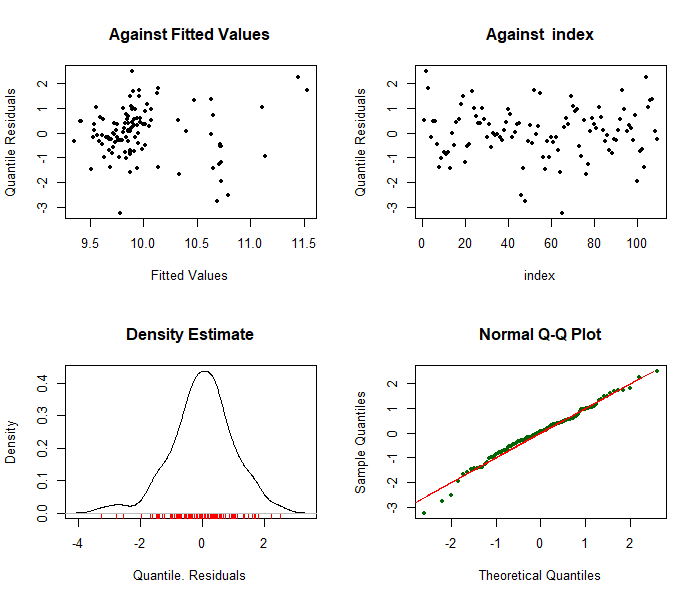
\includegraphics[width=0.95\linewidth]{figures/gamlss_residuals_kcc_6.png}
  \caption{Residuals of GAMLSS fit - KCC 6}
  \label{fig:gamlss_residuals_kcc_6}
\end{figure}


Inspecting the diagnostic plots for the residuals in \autoref{fig:gamlss_residuals_kcc_6} along with the associated summary in \autoref{tab:gamlss_residuals_kcc_6}, we can again confirm an appropriate fit. The plots in the upper row of \autoref{fig:gamlss_residuals_kcc_6} show how the points are scattered around (horizontal) zero without a clear pattern. The left lower plot resembles a normally distributed density curve adequately and the QQ-plot in the lower left corner displays the data matching to the diagona line. In \autoref{tab:gamlss_residuals_kcc_6}, metrics of the residuals are displayed. Those metrics indeed indicate an approximation of a standard normal distribution.  A Shapiro-Wilk test returns a p-value of 0.7, which is below the p-value of the fit without covariate effects. Nevertheless, normality is a steady assumption for the quantile residuals.
\\






\begin{table}[H]
\centering
\begin{tabular}{c}
\hline
\rowcolor{white} 
\textbf{Summary of the Quantile Residuals} \\ \hline\hline
 $\begin{array}[t]{ r @{{}={}} l }
\text{mean} & -0.01692598                         \\ 
\text{variance} & 1.011483                         \\ 
\text{coef. of skewness} & -0.1401063               \\ 
\text{coef. of kurtosis} & 3.144701                \\ \hline
\end{array}$
\end{tabular}
\caption{Residuals of GAMLSS Fit on KCC 2}
\label{tab:gamlss_residuals_kcc_6}
\end{table}


%\VerbatimInput[frame = single, label = "Residuals of GAMLSS Fit on KCC 6" ]{gamlss_residuals_kcc_6.txt}






%\inputRoutput[caption={Residuals of GAMLSS Fit on KCC 6},numbers=left,numberstyle=\tiny, label=output:gamlss_residuals_kcc_6]{gamlss_residuals_kcc_6.txt}

















\subsubsection{Key Category Cluster 8} \label{sssec:margin_kcc_8}
% !TEX root = Master.tex

The procedure is continued also for key category cluster 8 with the same conditions, since we have similar issues as in the previous two clusters.
\\

\autoref{tab:estimated_parameters_kcc_8_no_covariates}, \autoref{fig:kcc_8_margin} and \autoref{fig:res_kcc_8_no_covariates} summarize the findings when the log-sales of \ac{KCC} 8 are fitted to an ex-Gaussian distribution with no regressors. Normality of the residuals can be assumed, as the Shapiro-Wilk test returns a p-value of 0.99 and thus fails to reject the null hypothesis of non-normality.
\\



\begin{table}[H]
\setlength\arrayrulewidth{1pt}  
\centering
\begin{adjustbox}{max width=\textwidth}\
\begin{tabular}{|c|c|c|}
\hline
\rowcolor{lightgray} 
$\hat{\mu}$ & $\hat{\sigma}$ & $\hat{\nu}$ \\ \hline
7.21        & 0.27           & 0.46        \\ \hline
\end{tabular}
\end{adjustbox}
\caption{Estimated parameters for log-sales of KCC 8 fitted to ex-Gaussian distribution with no covariate effects}
\label{tab:estimated_parameters_kcc_8_no_covariates}
\end{table}



 \begin{figure}[H]
\centering
\begin{subfigure}{.45\textwidth}
  \centering
  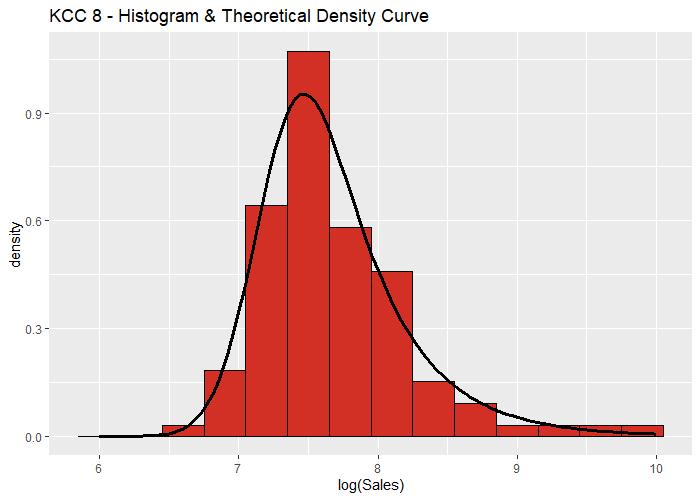
\includegraphics[width=\linewidth]{figures/kcc_8_density.png}
  \caption{Histogram \& theoretical density}
  \label{fig:kcc_8_density}
\end{subfigure}
\begin{subfigure}{.45\textwidth}
  \centering
  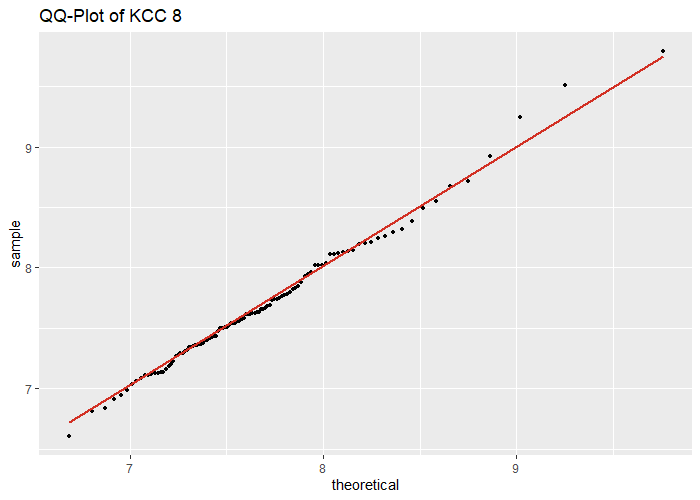
\includegraphics[width=\linewidth]{figures/kcc_8_qqplot.png}
  \caption{QQ-Plot}
  \label{fig:kcc_8_qqplot}
\end{subfigure}
\caption{ex-Gaussian distribution fitted to log-sales of \ac{KCC} 8}
\label{fig:kcc_8_margin}
\end{figure} 


\begin{figure}[H]
\centering
  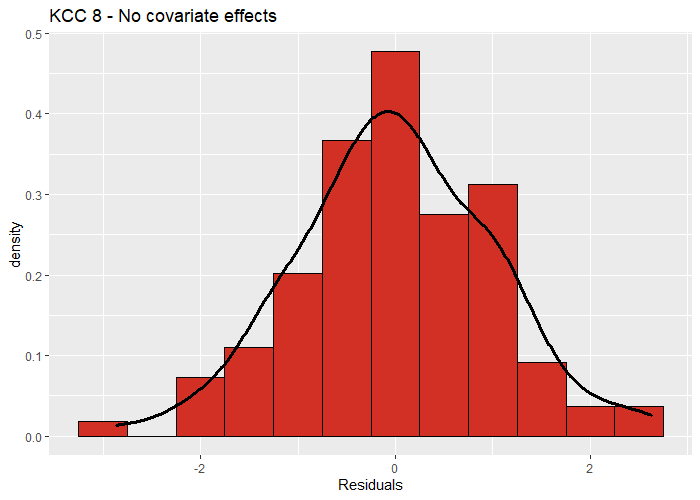
\includegraphics[width=0.45\linewidth]{figures/res_kcc_8_no_covariates.png}
  \caption{Residuals of KCC 8 log-sales fitted to an ex-Gaussian distribution with no covariate effects together with their density curve}
  \label{fig:res_kcc_8_no_covariates}
\end{figure}




Again, Model \ref{eq:gamlss_kcc_2} is applied to the log-sales. The summary output and estimated parameters with confidence intervals can be seen in \autoref{fig:gamlss_kcc_8_estimated_parameters} and in \autoref{tab:nu_ci_kcc_8}. We notice that models fit is acceptable matching the elevated sales during promo weeks and that the variability is strictly decreasing with the overall range having a range between 0.1 and 0.3. Skewness remains low in the data.
\\




%\VerbatimInput[frame = single, label = "GAMLSS Fit on KCC 8" ]{gamlss_fit_kcc_8_try1.txt}

\inputRoutput[caption={GAMLSS Fit on KCC 8}, numbers=left,numberstyle=\tiny, label=output:gamlss_fit_kcc_8_try1]{gamlss_fit_kcc_8_try1.txt}



\begin{figure}[H]
\centering
  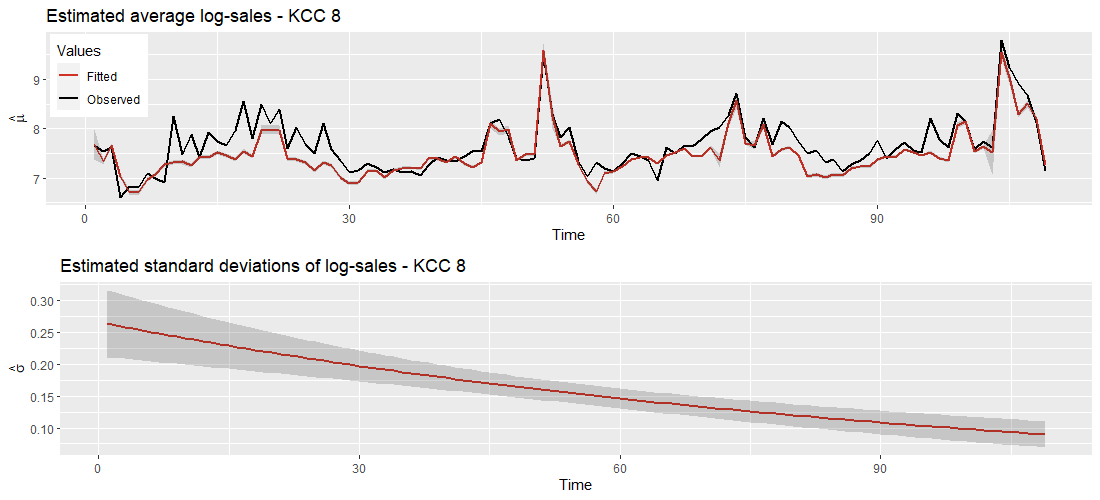
\includegraphics[width=0.95\linewidth]{figures/gamlss_kcc_8_estimated_parameters.png}
  \caption{Estimated location parameter $\hat{\mu}$ compared to the observed values and scale parameter $\hat{\sigma}$ with confidence bands of GAMLSS fit - KCC 8}
  \label{fig:gamlss_kcc_8_estimated_parameters}
\end{figure}



\begin{table}[H]
\setlength\arrayrulewidth{1pt}  
\centering
\begin{adjustbox}{max width=\textwidth}\
\begin{tabular}{|c|c|c|}
\hline
\rowcolor{lightgray} 
Lower & $\hat{\nu}$ & Upper \\ \hline
0.181        & 0.158           & 0.203        \\ \hline
\end{tabular}
\end{adjustbox}
\caption{Estimated skewness parameter $\hat{\nu}$ of GAMLSS fit with 95\% confidence interval bounds - KCC 8}
\label{tab:nu_ci_kcc_8}
\end{table}



Time as well as the total markdown percentage exhibit similar positive effects on the response as in \ac{KCC} 6, collapsing into a straight line. The promo effects seem to be more balanced, with different interquartile ranges for all cases.
\\


\begin{figure}[H]
\centering
  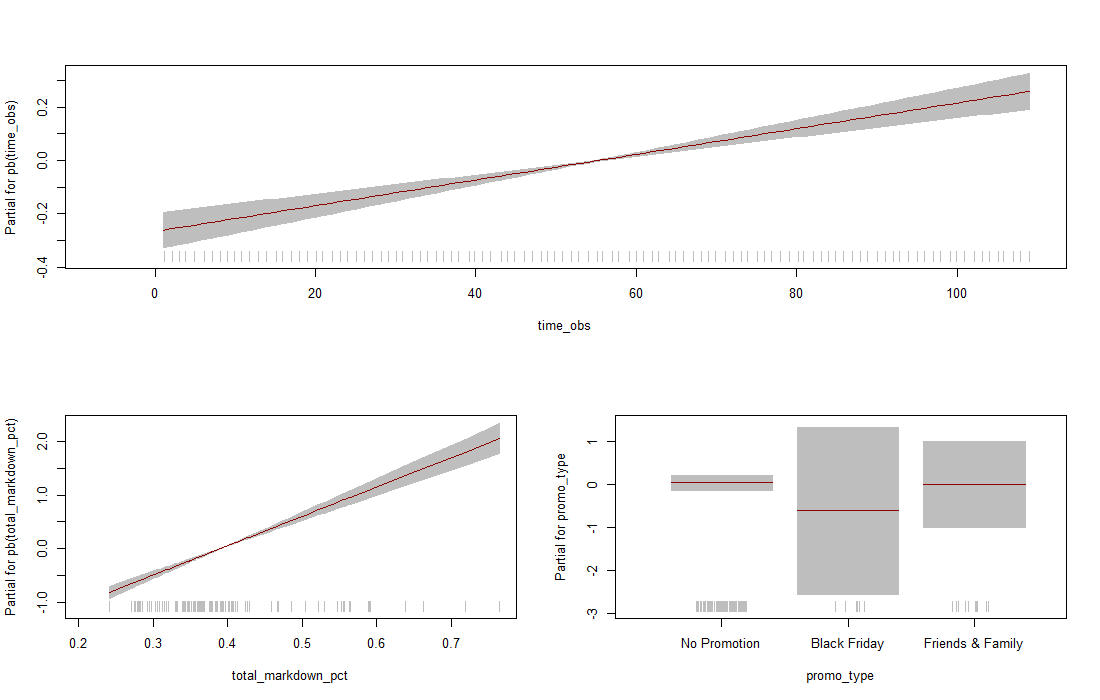
\includegraphics[width=0.95\linewidth]{figures/gamlss_effects_kcc_8.png}
  \caption{Covariate effects on the expected response variable (log-sales) of GAMLSS fit - KCC 8}
  \label{fig:gamlss_effects_kcc_8}
\end{figure}



Looking at \autoref{fig:gamlss_residuals_kcc_8} and R output \ref{output:gamlss_residuals_kcc_8} for the distribution of the quantile residuals, the fitting method for this cluster is also justified. The Shapiro-Wilk test is "weaker" in comparison to the fit without covariate effects with a p-value of 0.86, which is still a solid reason to retail the null hypothesis of normality.


\begin{figure}[H]
\centering
  \includegraphics[width=0.95\linewidth]{figures/gamlss_residuals_kcc_8.png}
  \caption{Residuals of GAMLSS fit - KCC 8}
  \label{fig:gamlss_residuals_kcc_8}
\end{figure}


%\VerbatimInput[frame = single, label = "Residuals of GAMLSS Fit on KCC 8" ]{gamlss_residuals_kcc_8.txt}

\inputRoutput[caption={Residuals of GAMLSS Fit on KCC 8},numbers=left,numberstyle=\tiny, label=output:gamlss_residuals_kcc_8]{gamlss_residuals_kcc_8.txt}




\subsection{Key Category Cluster - Pairwise Copulas}
\label{ssec:kcc_copulas}
% !TEX root = Master.tex

The next step, after fitting proper models to the marginal distributions of the log-sales aggregated on key category cluster level, is to enter the pairwise modelling of the clusters. Specifically, we are interested in capturing the dependence structure over time which is delineated in the next three Subsections (\ref{sssec:kcc_26}, \ref{sssec:kcc_28} and \ref{sssec:kcc_68}).
\\

Recalling the previous Section \ref{ssec:kcc_margins}, the residuals from the fitting method are depicted in \autoref{fig:res_gamlss_over_time} for each time-point. In a second step, the residuals will be used in a pairwise fashion after the marginal modelling to estimate the dependence structure with the help of conditional copulas (see Section \ref{ssec:conditional_copulas}).

\begin{figure}[H]
\centering
  \includegraphics[width=0.95\linewidth]{figures/res_gamlss_over_time.png}
  \caption{Estimated residuals of GAMLSS fits for the three key category clusters}
  \label{fig:res_gamlss_over_time}
\end{figure}






\inputRoutput[caption={AIC values of distribution fits on KCC with \textit{fitDist()} function of the \textit{gamlss} package},numbers=left,numberstyle=\tiny, label=output:gamlss_distributions_aic]{gamlss_distributions_aic.txt}



In the previous Section \ref{ssec:kcc_margins}, the model fits resulted in quantile residuals that we were able to approximate parametrically by normal distributions. When the three sets of residuals are passed into the \textit{fitDist()} function of the \textit{gamlss} package, it returns multiple suggestions of parametric distribution that can be used to fit to the data, ordered by ascending \ac{AIC}. An excerpt is given in R output \ref{output:gamlss_distributions_aic}. The only distributions that are also at the disposal of the \textit{gjrm} package\footnote{Elaboration on this in the following subsections.} are the normal and the logistic distributions and the \ac{AIC} values are close, indicating that both are good fits. Thus, the normal distribution is chosen for all three residual sets in the following.




%\subsection{KCC Correlations} \label{ssec:kcc_correlations}
%% !TEX root = Master.tex

Starting the dependence modelling on the key category cluster level, we will be aiming for obtaining separate estimations of pairwise correlations over time, as we only have 3 nodes on this level and manual approximation is feasible on this low number of dimensions. %Since large outliers are involved and we assume to be dealing with tail dependence, we use Kendall's tau rank correlation coefficients for comparison (see Section \ref{sssec:rank_correlation}). 
For the next three Subsections (\ref{sssec:kcc_26}, \ref{sssec:kcc_28} \& \ref{sssec:kcc_68}), we will compare resulting dependence structures inheriting from different approaches introduced in this Section.\\

There is an inevitable challenge when it comes to estimating and projecting summary metrics like correlation coefficients onto every observation point; they cannot be tested and thus fully reliable assessments are not guaranteed. Therefore, we will be interpreting the results by comparing several frameworks \textit{under feasibly similar conditions}.\\


\textbf{Generalized Additive Models for Conditional Dependence structures (gamCopula)}\\
We will be taking advantage of the framework of \textit{Generalized Additive Models for Conditional Dependence Structures} introduced in \cite{vatter2015generalized} to account for predictor effects on the dependence measure.\footnote{In the scope of this thesis, by dependence we mean concordance and do not distinguish between those terms as opposed to the reference.} The R implementation for this framework and its extension to Pair-Copula Constructions \citep{vatter2018generalized} can be utilized by the \textit{gamCopula} package \citep{vatter2019gamcopula}. \\

%Before we fit the models, some clarifications regarding the predictors should be pointed out. As we aggregate the dataset from article level to \ac{KCC} level:
%\begin{itemize}
%\item promotion intensities \textit{bf\_w} and \textit{ff\_w} become binary, with 1 indicating presence of the respective promo week (see Tables \ref{tab:black_friday} and \ref{tab:friends_and_family}) and 0 otherwise
%\item the individual total markdown percentages for each \ac{KCC} are %all averaged together as they are pairwise highly correlated with slopes close to one (see \autoref{fig:total_markdown_pct_kcc}). This holds of course for the "gamCopula" approach only.
%\end{itemize}

%With the help of the function \textit{gamBiCopSelect} of the \textit{gamCopula} package, we can estimate the parameters of bivariate copulas for a given set of copula families. 
The copula parameter estimates are obtained by maximum likelihood estimation, where each iteration is reformulated as a generalized ridge regression solved using the \textit{mgcv} package \citep{wood2017generalized}. The Fisher scoring method is employed, as the results turn out to be more stable and in greater alignment with other approaches (for more details, see \cite{vatter2018generalized}).  We choose \ac{AIC} for the bivariate copula selection and set the maximal number of Newton-Raphson iterations to 100 so that the algorithm converges for all cases.  \\
The model setup is as follows: 

\begin{equation}
\tau(z) = \frac{exp(z) - 1}{exp(z) + 1},
\label{eq:tau_link}
\end{equation}
where
\begin{equation}
z = \beta_0 + \beta_1 \textit{bf} + \beta_2 \textit{ff} + f(\textit{time}) + f(\textit{total\_markdown\_pct})
\label{eq:gam_kcc}
\end{equation}
when using the bivariate (pairwise) pseudo observations $z$ of the marginals as model responses. This allows for flexible estimation of the copula parameter $\theta$ and therefore also Kendall's tau (see Section \ref{sssec:rank_correlation}) which is dependent on time. For all three pairs, the selected copula is the Student's t-copula. The t-copula is indeed found to be the most appropriate copula family after testing other families as well (like Normal or Gumbel copula) and is capturing tail dependencies adequately well (see Section \ref{sssec:elliptical_copulas}), not only in the scope of this approach. \\
As stated in \autoref{eq:kendall_to_copula}, the copula is sufficient for directly deriving the correlation coefficient. The smooth functions for time and total markdown percentage in \autoref{eq:gam_kcc} are constructed using thin plate regression splines and by setting 26 and 10 knots respectively, whereas the promotion indicators are set as linear covariates. Results should however be treated with caution, as the algorithm does not converge for all cases. 
%The only cases where we achieve convergence are the pairs KCC 2 \& KCC 8 as well as KCC 6 \& KCC 8.


\hfill $\square$ \\


% NOTE THAT ONLY FOR THIS PICTURE WE USE THE PNG FORMAT. THE "alpha" TRANSPARENCY WILL NOT SHOW WITH EPS FORMAT...
%\begin{figure}[H]
%\centering
%  \includegraphics[width=0.9\linewidth]{figures/%total_markdown_pct_kcc.png}
%  \caption{Pairwise total markdown percentages of the key category %clusters (scatterplots, densities \& linear correlations)}
%  \label{fig:total_markdown_pct_kcc}
%\end{figure}


\textbf{Generalized Joint Regression Models (GJRM)}\\
This approach is based on the framwork of \textit{\ac{GJRM}} and its implementations in R \citep{marra1605bivariate, marragjrm}, where the scope of \ac{GAMLSS}, which was first introduced by \cite{rigby2005generalized}, is extended by a bivariate copula model. The framework represents the frequentist counterpart of \cite{klein2016simultaneous} and parameter estimation is achieved within a penalized likelihood framework by using a trust region algorithm (see \cite{marragjrm} for more details). \\

To set similar conditions on the fitting part, we use again a Student's t copula which again provides the most stable results. The marginals are of course assumed to be Dagum distributed (see Section \ref{ssec:kcc_marginals}). As we are primarily interested in the dependence structure, we will not be using covariate effects for any model parameters except for the copula parameter (and consequently the dependence measure). 
%As a matter of fact, the results are barely affected. 
So essentially, besides the constant model parameters, we have 
\begin{equation}
\theta = \beta_0 + \beta_1 \textit{bf} + \beta_2 \textit{ff} + f(\textit{time}) + f(\textit{total\_markdown\_pct})
\label{eq:gjrm_kcc}
\end{equation}
with link function for $\theta$ 
\begin{equation}
\theta = arctanh(\rho) = \frac{1}{2} ln (\frac{1 + \rho}{1 - \rho}).
\label{eq:theta_link}
\end{equation}\\

Optionally, we can convert $\rho$ to Kendall's tau via

$$
\tau = \frac{2}{\pi}arcsin(\rho)
$$
(see \autoref{tab:copula_relationships}). \\

The parameter $\theta$ from \autoref{eq:gjrm_kcc} is in this case being mapped to Pearson's correlation coefficient $\rho$ via \autoref{eq:theta_link} due to the t-copula. The additive model structure of \autoref{eq:gjrm_kcc} with the copula parameter as response matches \autoref{eq:gam_kcc} regarding the linear predictor, i.e. linear effects as well as smooth functions and their respective number of knots. Again, we should treat the outcome with caution as the algorithm fails to converge for all cases. Convergence failure may have various reasons, e.g. low sample size compared to complexity of the model or model misspecification. Unfortunately, not a single model configuration accomplished convergence so we carefully interpret the outcomes in the below Subsections.


\hfill $\square$ \\













\subsubsection{Key Category Clusters 2 \& 6} \label{sssec:kcc_26}
% !TEX root = Master.tex

To start things off, a look at the scatterplot in \autoref{fig:scatter_res_kcc_26} between the residuals of \ac{KCC} 2 \& \ac{KCC} 6 provides a first hint of a potential correlation structure. For the most part, the data looks quite elliptically scattered. Thus, a normal or a t-copula should be appropriate copulas to be used.
\\


\begin{figure}[H]
\centering
  \includegraphics[width=0.45\linewidth]{figures/scatter_res_kcc_26.png}
  \caption{Scatterplot of estimated residuals of GAMLSS fits for key category clusters 2 \& 6}
  \label{fig:scatter_res_kcc_26}
\end{figure}


The selected copula is a t-copula with 3.17\footnote{Estimation returns degrees of freedom as positive real values above 2 instead of just integer values.} \ac{dof} and the Pearson's rho as well as Kendall's tau correlation coefficients coincide with the empirical sample coefficients of 0.49 and 0.3 respectively. A short explanation about the selection of the copula can be found in the \nameref{sec:appendix}.
\\
Furthermore, to estimate the copula parameter flexibly over time, the \ac{GJRM} framework introduced by \cite{marra1605bivariate} is utilized\footnote{See Section \ref{ssec:conditional_copulas} as well as the referred paper.}. Essentially, the scope of the \ac{GAMLSS} framework is extended to a bivariate copula additive model, where all parameters of the margins as well as the copula parameter can be estimated simultaneously using structured additive predictors. The parameters are estimated within a penalized likelihood framework using a trust region algorithm with integrated automatic smoothing parameter selection (More details can be found in \cite{marra1605bivariate}). This framework has been implemented in R by \cite{marragjrm} within the scope of the \textit{GJRM} package. \\
Given the \ac{GAMLSS} fit residuals of key category clusters 2 \& 6 acting as marginal Gaussian response inputs, as well as a t-copula with the above mentioned degrees of freedom as starting value, the formula specification is as follows: \\



\begin{equation}
\begin{array}{c}
\mu_{KCC 2}=\beta_{\mu,KCC2} \qquad \mu_{KCC 6}=\beta_{\mu,KCC6}  \\  \noalign{\vskip5pt}

log(\sigma_{KCC 2})=\beta_{\sigma,KCC2} \qquad log(\sigma_{KCC 6})=\beta_{\sigma,KCC6} \\  \noalign{\vskip5pt}

log(\nu) = \beta_{\nu} \\  \noalign{\vskip5pt}

tanh^{-1}(\theta)=\beta_{\theta} + \textit{promo\_type} +f(\textit{time}),
\end{array}
\label{eq:gjrm_formula_26}
\end{equation} 
where $\nu$ denotes the degrees of freedom of the t-copula, $tanh^{-1}$ is the inverse hyperbolic tangent function\footnote{Defined as $\tanh ^{-1} (x)=\frac{1}{2} \ln \left(\frac{1+x}{1-x}\right)$ on the domain $ \{ x \in \mathbb{R}:-1<x<1\}$.} relating the expected value of the copula parameter $\hat{\theta}$ to the additive predictor $\beta_{\theta}+ \textit{promo\_type} +f\left(\textit{time}\right)$ and $f$ being a smooth function build upon thin plate regression splines and 30 equidistant knots \citep{wood2017generalized}. Note that, as the chosen copula is a Student's t-copula, $\theta$ equates Pearson's correlation coefficient $\rho$. The rest of the model parameters are all set as constant values as the model seems to be robust to any changes including covariates. Incorporating covariates within smooth functions with high numbers of knots on the contrary lead to less reliable estimations (especially due to increasing number of parameters compared to this sample size). The promo types don't seem to be significant for the correlation structure, as can be seen in \autoref{tab:theta_coeff_kcc_26}. The smooth component (time) has significant 20.44 effective degrees of freedom (edf), which is reflected also in the wiggliness of the time effect (see \autoref{fig:time_effect_on_theta_26}). A detailed summary output of the model fit can be found in the \nameref{sec:appendix}. \\




\begin{table}[H]
\centering
\begin{tabular}{l|c|c|c|c}
\hline
                               \textbf{$\hat{\theta}$ Coefficients}       & \textbf{Estimate} & \textbf{Std. Error} & \textbf{z value} & \textbf{p-value}  \\ \hline\hline
$\beta_{\theta}$ \textit{(Intercept)}                  & 0.88     & 0.12       & 7.36    & 0.00 *** \\ 
\textit{promo\_typeBlack Friday}      & -0.87    & 0.74       & -1.19   & 0.24     \\ 
\textit{promo\_typeFriends \& Family} & -0.65    & 0.38       & -1.71   & 0.09 .   \\ \hline
& & & & \\ \hline
\textbf{Smooth components}            & \textbf{edf}      & \textbf{Ref.df}     & \textbf{Chi.sq}  & \textbf{p-value}  \\ \hline\hline
\textit{$f$(time)}                 & 20.44    & 23.79      & 63.54   & 0.00 *** \\ \hline
\end{tabular}
\caption{Estimated $\hat{\theta}$ coefficients of \ac{GJRM} fit on key category clusters 2 \& 6}
\label{tab:theta_coeff_kcc_26}
\end{table}



Model \ref{eq:gjrm_formula_26}, along with the mentioned prespecified settings, generates a good overall fit, which is confirmed when checking the histogram and the QQ-plots of the quantile residuals for the two margins (see \autoref{fig:res_hist_qqplot_26}). The histograms and the density curves convincingly indicate normal distributions and the QQ-plots match the $y=x$ lines fairly well. 
\\


\begin{figure}[H]
\centering
  \includegraphics[width=0.80\linewidth]{figures/res_hist_qqplot_26.png}
  \caption{Diagnostic plots of quantile residuals based on \ac{GJRM} models for key category clusters 2 \& 6}
  \label{fig:res_hist_qqplot_26}
\end{figure}



The effect of time on the copula parameter can be viewed in \autoref{fig:time_effect_on_theta_26}, where the number 20.44 in brackets on the y-axis denotes the effective degrees of freedom (see \autoref{tab:theta_coeff_kcc_26}) of the smooth curve, which is centered around zero due to identifiability constraints.
\\

\begin{figure}[H]
\centering
  \includegraphics[width=0.95\linewidth]{figures/time_effect_on_theta_26.png}
  \caption{Estimated Smooth effect of time on the copula parameter $\theta$ with 95\% confidence bands for key category clusters 2 \& 6}
  \label{fig:time_effect_on_theta_26}
\end{figure}



\autoref{fig:estimated_theta_kcc_26} displays the correlation between the two margins which highly fluctuates between (almost) perfect negative and positive dependence, suggesting that only copulas which can account for both of those dependence (concordance) types should be considered. Candidate copulas were the Frank copula, the Ali-Mikhali-Haq copula and Fari-Gumbel-Morgenstern copula, where the last two can only account for weak dependencies \citep{marra1605bivariate}. The Student's t-copulas provides the most appropriate fit among those types of copulas so we stick to it. The width of the confidence intervals also does vary a lot across different parts of the observation period. \\



\begin{figure}[H]
\centering
  \includegraphics[width=0.95\linewidth]{figures/estimated_theta_kcc_26.png}
  \caption{Estimated copula parameter over time and 95\% confidence bands from a \ac{GJRM} t-copula model with normal margins for key category clusters 2 \& 6 - Season type in the background - Dashed horizontal line at $\hat{\theta} = 0$}
  \label{fig:estimated_theta_kcc_26}
\end{figure}
%  - Confidence bands are neglected for clarity of the graph



Positive correlation in a business context would mean that, for both clusters, sales are increasing conjointly. Negative correlations (below dashed line of \autoref{fig:estimated_theta_kcc_26}) indicate that, as one's cluster's sales increase, the other one's drop and further questioning should be carried out. We see such negative correlations during the Spring-Summer seasons and somewhat during Black Friday towards the end of Fall-Winter 2017.


%We will start the pairwise analysis with inspecting the \ac{GJRM} approach. As mentioned above, the margins are specified as Dagum distributed \acp{RV} and we choose the Student's t copula (the degrees of freedom do not affect the outcome, as they just serve as starting values for \ac{GAMLSS} estimation). All model parameters are set to constant, except the copula parameter (which is defined as in \autoref{eq:gjrm_kcc}). These settings also hold for Subsections \ref{sssec:kcc_28} and \ref{sssec:kcc_68}. We can see in the diagnostic plots of \autoref{fig:margin_estimates_kcc_26} that this type of model fitting returns quite successful results. \\
%
%\begin{figure}[H]
%\centering
%  \includegraphics[width=0.9\linewidth]{figures/margin_estimates_kcc_26.eps}
%  \caption{Estimation diagnostics for the response margins KCC 2 \& KCC 6; \ac{GJRM} approach}
%  \label{fig:margin_estimates_kcc_26}
%\end{figure}
%
%Regarding the fitting of the copula parameter $\rho$, time-varying estimation is achieved. The red line in \autoref{fig:copula_parameters_26} shows the estimated time-dependent sequence of $\hat{\rho}$, where an instant positive conclusion is that the outcome is very close to the gamCopula approach. This indicates that the model setup of these two approaches both agree for the most part on the dependence structure. (Confidence intervals of the lines are not shown to retain clarity in the figure).\\
%
%
%\begin{figure}[H]
%\centering
%  \includegraphics[width=0.9\linewidth]{figures/copula_parameters_26.eps}
%  \caption{Estimated time-varying Pearson's correlation coefficients for the pair KCC 2 \& KCC 6}
%  \label{fig:copula_parameters_26}
%\end{figure}
%
%
%By large, the dependence is constantly at a very high positive level, with a noticeable turn in high negativity during the summer months of 2017. The gamCopula approach seems to pick up slightly more regional fluctuations than the \ac{GJRM} approach.







\subsubsection{Key Category Clusters 2 \& 8} \label{sssec:kcc_28}
% !TEX root = Master.tex

The same strategy as in the previous subsection (\ref{sssec:kcc_26}) shall be followed. In \autoref{fig:scatter_res_kcc_28}, a lower tail dependence can be suspected. Whether both positive and negative dependencies are hiding in the the data is being tested beforehand, so that we can narrow down the number of plausible copula families.
\\

\begin{figure}[H]
\centering
  \includegraphics[width=0.45\linewidth]{figures/scatter_res_kcc_28.png}
  \caption{Scatterplot of estimated residuals of GAMLSS fits for key category clusters 2 \& 8}
  \label{fig:scatter_res_kcc_28}
\end{figure}


A \ac{GJRM} approach equivalent to Model \ref{eq:gjrm_formula_26} is applied here, with the only difference that we leave out the promo type (see Model \ref{eq:gjrm_formula_28}) since it not only has a non-significant effect, but unlike for the previous pair it also heavily distorts the outcome for this pair. 
\begin{equation}
\begin{array}{c}
\mu_{KCC 2}=\beta_{\mu,KCC2} \qquad \mu_{KCC 6}=\beta_{\mu,KCC6}  \\  \noalign{\vskip5pt}

log(\sigma_{KCC 2})=\beta_{\sigma,KCC2} \qquad log(\sigma_{KCC 6})=\beta_{\sigma,KCC6} \\  \noalign{\vskip5pt}

log(\nu) = \beta_{\nu} \\  \noalign{\vskip5pt}

tanh^{-1}(\theta)=\beta_{\theta}  +f(\textit{time})
\end{array}
\label{eq:gjrm_formula_28}
\end{equation} 
All model parameters but the copula parameter are set as constants. Since a t-copula is again applied, the copula parameter obtains an inverse hyperbolic tangent function as link. Also, time is the only covariate in Model \ref{eq:gjrm_formula_28}. \\
A summary about the coefficients of the estimated copula parameter $\hat{\theta}$ is printed in \autoref{tab:theta_coeff_kcc_28}.  We first examine copulas which account for positive as well as negative dependencies.\footnote{With the help of the \textit{BiCopSelect()} function of the \textit{VineCopula} package \citep{nagler2019vinecopula}.} The t-copula is again the most appropriate within a set of copula families including the independence copula, the Gaussian copula, the Student's t-copula and the Frank copula. Looking at \autoref{tab:theta_coeff_kcc_28}, we can see that time has a significant non-linear effect on $\hat{\theta}$ (18.50 edf) and its partial smooth effect can be checked visually in \autoref{fig:time_effect_on_theta_28}.
\\



\begin{table}[H]
\centering
\begin{tabular}{l|c|c|c|c}
\hline
                               \textbf{$\hat{\theta}$ Coefficients}       & \textbf{Estimate} & \textbf{Std. Error} & \textbf{z value} & \textbf{p-value}  \\ \hline\hline
$\beta_{\theta}$ \textit{(Intercept)}                  & 0.64     & 0.11       & 5.82    & 0.00 ***   \\ \hline
& & & & \\ \hline
\textbf{Smooth components}            & \textbf{edf}      & \textbf{Ref.df}     & \textbf{Chi.sq}  & \textbf{p-value}  \\ \hline\hline
\textit{$f$(time)}                 & 18.50    & 21.75      & 41.44   & 0.01 ** \\ \hline
\end{tabular}
\caption{Estimated $\hat{\theta}$ coefficients of \ac{GJRM} fit on key category clusters 2 \& 8}
\label{tab:theta_coeff_kcc_28}
\end{table}











\begin{figure}[H]
\centering
  \includegraphics[width=0.95\linewidth]{figures/time_effect_on_theta_28.png}
  \caption{Estimated Smooth effect of time on the copula parameter $\theta$ with 95\% confidence bands for key category clusters 2 \& 8}
  \label{fig:time_effect_on_theta_28}
\end{figure}





\begin{figure}[H]
\centering
  \includegraphics[width=0.80\linewidth]{figures/res_hist_qqplot_28.png}
  \caption{Diagnostic plots of quantile residuals based on \ac{GJRM} models for key category clusters 2 \& 8}
  \label{fig:res_hist_qqplot_28}
\end{figure}

The parsimonious model setup produces a nice fit. The quantile residuals are remarkably close to a standard normal distribution, which is reflected in the histograms and QQ-plots of both margins in \autoref{fig:res_hist_qqplot_28}.\\
Consequently, we proceed to analyzing the correlation parameter. Once again, $\hat{\theta}$ takes on positive as well as negative values interchangeably over time periods. Therefore, considering further copula families like the Clayton copula would be arguably inappropriate.
\\


Looking at the correlation structure in \autoref{fig:estimated_theta_kcc_28}, we can see that during both mid-seasons of Fall-Winter 2017 and 2018 there is some negative dependence between the two clusters. End of Spring-Summer 2017 and beginning of Spring-Summer 2018 also show some negative correlation.
\\

\begin{figure}[H]
\centering
  \includegraphics[width=0.95\linewidth]{figures/estimated_theta_kcc_28.png}
  \caption{Estimated copula parameter over time and 95\% confidence bands from a \ac{GJRM} t-copula model with normal margins for key category clusters 2 \& 8 - Season type in the background - Dashed horizontal line at $\hat{\theta} = 0$}
  \label{fig:estimated_theta_kcc_28}
\end{figure}
%  - Confidence bands are neglected for clarity of the graph














%On this \ac{KCC} pair, the \ac{GJRM} approach is not as favorable as in the pair KCC 2 \& KCC 6, though it might be considered acceptable (\autoref{fig:margin_estimates_kcc_28}).  \\
%
%\begin{figure}[H]
%\centering
%  \includegraphics[width=0.9\linewidth]{figures/margin_estimates_kcc_28.eps}
%  \caption{Estimation diagnostics for the response margins KCC 2 \& KCC 8; \ac{GJRM} approach}
%  \label{fig:margin_estimates_kcc_28}
%\end{figure}
%
%This circumstance is reflected within the comparison of the "gamCopula" estimated dependence measures. The overall similarity between the two lines in \autoref{fig:copula_parameters_28}, which depict the time-dependent correlation parameters of this pair, is given. However, the details reveal that there are severe differences between the estimation methods. As the gamCopula approach yields converge in contrast to the \ac{GJRM} method, it might be preferential. Nevertheless, the results should be treated with adequate caution.
%
%\begin{figure}[H]
%\centering
%  \includegraphics[width=0.9\linewidth]{figures/copula_parameters_28.eps}
%  \caption{Estimated time-varying Pearson's correlation coefficients for the pair KCC 2 \& KCC 8}
%  \label{fig:copula_parameters_28}
%\end{figure}
%
%
%The stretched sign change of the correlation over time happens, just like in the previous pair, from June to August 2017. The curves here are surprisingly different in terms of their stability. The gamCopula method seems to have a more stable course compared to the \ac{GJRM} approach. The red line in \autoref{fig:copula_parameters_28} appears very sensitive in very short time intervals.




\subsubsection{Key Category Clusters 6 \& 8} \label{sssec:kcc_68}
% !TEX root = Master.tex



This pair of clusters also let's us speculate whether tail dependence exists (see \autoref{fig:scatter_res_kcc_68}).
\\


\begin{figure}[H]
\centering
  \includegraphics[width=0.45\linewidth]{figures/scatter_res_kcc_68.png}
  \caption{Scatterplot of estimated residuals of GAMLSS fits for key category clusters 6 \& 8}
  \label{fig:scatter_res_kcc_68}
\end{figure}


This time, we fast forward to the outcome when a t-copula is applied (which is the proposed family of copulas allowing both concordance directions) under similar conditions as in Model \ref{eq:gjrm_formula_28} (the reasons for leaving out promo type being the same as in Subsection \ref{sssec:kcc_28}). Interestingly, the correlation parameter seems to be purely non-negative
%\footnote{Without considering the lower confidence bounds in the first part of the time window.} 
(see \autoref{fig:estimated_theta_t_copula_kcc_68}).
\\


\begin{figure}[H]
\centering
  \includegraphics[width=0.95\linewidth]{figures/estimated_theta_t_copula_kcc_68.png}
  \caption{Estimated copula parameter over time from a \ac{GJRM} t-copula model with normal margins for key category clusters 6 \& 8 with 95\% confidence bands}
  \label{fig:estimated_theta_t_copula_kcc_68}
\end{figure}


Keeping the complexity of the model to a minimum, the model setup remains as is, with only minor differences. Other copula families are considered in addition, particularly those that account for positive (and not negative) dependencies. Out of all implemented copula families in the \textit{VineCopula} package (rotated versions included, see \cite{nagler2019vinecopula}), the Clayton copula yields the most fitting family for the given target variables. This result is sensible, as the Clayton copula is able to capture lower tail dependencies (see \autoref{fig:scatter_res_kcc_68}) and accounts for positive dependence structures only (see Subsections \ref{sssec:archimedean_copulas} and \ref{sssec:tail_dependence}). Note that the new model specification is 
\begin{equation}
\begin{array}{c}
\mu_{KCC 6}=\beta_{\mu,KCC6} \qquad \mu_{KCC 8}=\beta_{\mu,KCC8}  \\  \noalign{\vskip5pt}

log(\sigma_{KCC 6})=\beta_{\sigma,KCC6} \qquad log(\sigma_{KCC 8})=\beta_{\sigma,KCC8} \\  \noalign{\vskip5pt}


log(\theta)=\beta_{\theta}+f\left(\textit{time}\right),
\end{array}
\label{eq:gjrm_formula_68}
\end{equation}
where now there are no degrees of freedom to determine and the copula parameter receives a logarithmic link function to ensure that $\hat{\theta}$ is well defined on the non-negative real line. \autoref{tab:theta_coeff_kcc_68} displays the significance of the smooth effect of time on $\hat{\theta}$ having 21.88 effective degrees of freedom. The smooth effect of time on the copula parameter $\hat{\theta}$ with 95\% confidence bands is depicted in \autoref{fig:time_effect_on_theta_68}. Overall, the effect seems to be constant until mid of Fall-Winter 17, where a sudden drop is visible. Afterwards, it increases again to the same level as before and remains constant.



\begin{table}[H]
\centering
\begin{tabular}{l|c|c|c|c}
\hline
                               \textbf{$\hat{\theta}$ Coefficients}       & \textbf{Estimate} & \textbf{Std. Error} & \textbf{z value} & \textbf{p-value}  \\ \hline\hline
$\beta_{\theta}$ \textit{(Intercept)}                  & -8.24     & 3.77       & -2.19    & 0.03 *   \\ \hline
& & & & \\ \hline
\textbf{Smooth components}            & \textbf{edf}      & \textbf{Ref.df}     & \textbf{Chi.sq}  & \textbf{p-value}  \\ \hline\hline
\textit{$f$(time)}                 & 21.88    & 23.85      & 1560   & 0.00 *** \\ \hline
\end{tabular}
\caption{Estimated $\hat{\theta}$ coefficients of \ac{GJRM} fit on key category clusters 6 \& 8}
\label{tab:theta_coeff_kcc_68}
\end{table}



\begin{figure}[H]
\centering
  \includegraphics[width=0.95\linewidth]{figures/time_effect_on_theta_68.png}
  \caption{Estimated Smooth effect of time on the copula parameter $\theta$ with 95\% confidence bands for key category clusters 6 \& 8}
  \label{fig:time_effect_on_theta_68}
\end{figure}







\begin{figure}[H]
\centering
  \includegraphics[width=0.80\linewidth]{figures/res_hist_qqplot_68.png}
  \caption{Diagnostic plots of quantile residuals based on \ac{GJRM} models for key category clusters 6 \& 8}
  \label{fig:res_hist_qqplot_68}
\end{figure}




The diagnostic plots of quantile residuals in \autoref{fig:res_hist_qqplot_68} demonstrate the proper fit qualities once more. The histograms of the residuals and the associated density curves resemble the shape of normal distributions and the points on the QQ-plots match the diagonal lines almost perfectly. 
\\



Since Kendall's tau is more intuitive as a dependence measure of two random variables than the copula parameter $\theta$ (see Subsection \ref{sssec:rank_correlation}), this is what we inspect. The relationship between Kendall's tau and the parameter of the Clayton copula is $\tau = \frac{\theta}{\theta + 2}$ (see \autoref{tab:copula_relationships}). The estimated time-varying $\hat{\tau}$ is displayed in \autoref{fig:estimated_tau_clayton_kcc_68}, where we can observe that 
%the confidence bands vary a lot and 
there are some individual time windows of zero correlation.\\
Any model configuration of this pair regarding covariates and copulas produce such kind of strictly non-negative dependence. These results should be interpreted with extraordinary caution if at all.
\\



\begin{figure}[H]
\centering
  \includegraphics[width=0.95\linewidth]{figures/estimated_tau_clayton_kcc_68.png}
  \caption{Estimated Kendall's tau over time and 95\% confidence bands from a \ac{GJRM} Clayton copula model with normal margins for key category clusters 6 \& 8 - Season type in the background - Dashed horizontal line at $\hat{\theta} = 0$}
  \label{fig:estimated_tau_clayton_kcc_68}
\end{figure}
% - Confidence bands are neglected for clarity of the graph

































%The \ac{GJRM} fit on this pair seems to work just fine, which is underlined when observing \autoref{fig:margin_estimates_kcc_68}. As for the estimation of the dependence, we obtain a similar scheme as in the pair \ac{KCC} 2 \& \ac{KCC} 8. The main course of the correlation coefficient is common for both approaches, however the gamCopula approach seems to reveal heavier fluctuations. As always, it shall be stressed that these conclusions should be taken into account with extra caution, as both algorithms converge.
%
%\begin{figure}[H]
%\centering
%  \includegraphics[width=0.9\linewidth]{figures/margin_estimates_kcc_68.eps}
%  \caption{Estimation diagnostics for the response margins KCC 6 \& KCC 8; \ac{GJRM} approach}
%  \label{fig:margin_estimates_kcc_68}
%\end{figure}
% 
%
%
%
%\begin{figure}[H]
%\centering
%  \includegraphics[width=0.9\linewidth]{figures/copula_parameters_68.eps}
%  \caption{Estimated time-varying Pearson's correlation coefficients for the pair KCC 6 \& KCC 8}
%  \label{fig:copula_parameters_68}
%\end{figure}
%
%
%
%In both correlations in \autoref{fig:copula_parameters_68} show an overall increasing trend from the start, which stabilizes somewhere in September of 2017. Both curves return positive values throughout the entire time span (except for the very start of the black one). Also, wider and heavier fluctuations occur in the gamCopula approach as opposed to the \ac{GJRM} method, which looks much smoother.
\subsection{Article Dependencies} \label{ssec:article_dependencies}
% !TEX root = Master.tex

Dependence structures over time for aggregate sets of sales data have been analyzed so far and measures of dependence (or concordance) were sought after, usually in the context of correlation with values between $-1$ and $1$ indicating the magnitude. Parametric approaches were performed to obtain comprehensible results. However, entering the lowest level of granularity of target objects, namely the individual articles themselves (see \autoref{fig:article_hierarchy}), there are some heavy drawbacks as discussed in Section \ref{ssec:individual_patterns}.
\\

Within the scope of Section \ref{ssec:kcc_copulas}, an important aspect needs to be taken into consideration. That is the well known fact that correlation does not imply causation. Therefore, other frameworks which enable us to detect causal effects and maybe even allow approximate quantification\footnote{e.g. Sales transferability from one article to another (over time).} shall be briefly discussed in this Section and serve as possible directions for further investigation.
\newpage
\thispagestyle{empty}
\cleardoublepage


% Now clear headnotes again and get settings
%\fancyhf{}
%\fancyhead[LO,RE]{\footnotesize \nouppercase{\leftmark}}
%\fancyhead[RO,LE]{\footnotesize \thepage}


\thispagestyle{plain}
\section{Conclusion} \label{sec:conclusion}
%% !TEX root = Master.tex

The objective of this study is to contribute to the development of LiDAR assisted forest inventories by developing
a statistical sound approach to derive unbiased diameter distribution models from LiDAR data for homogeneous
compartments of the forest. Prediction is successfully performed by a generalized linear
regression model using the gamma distribution with log as a link function. Clustering the compartments into three groups led to enough samples per cluster to
perform distribution engineering. Clustering is not meant to find groups upon a decision for more or less correction is made, but
to find an appropriate correction for similar compartments. Clustering further uncovered the issue of not detecting
equally height trees, which introduced additional bias in the tree diameter prediction. Bias correction is
achieved by fitting a gamma distribution on the diameter distribution of each cluster from the inventory dataset
and subsequently the predicted diameter distribution. A correction factor is calculated based on the ratio of the
shape and scale parameter of both fitted distributions for each cluster. High confidence is thus given to the
inventory dataset. Subsequently, the correction factor is applied for each section. \\

This approach could solve all present challenges, without relying on any heuristic methods apart from choosing
an appropriate amount of clusters and variables. Hence the objective of finding a statistical sound approach is achieved.\\

We could not find studies with similar approaches to the objective. 
The achieved residual standard error of the mean diameter of the corrected compartment distribution of 5.49cm (see Section \ref{Results}) is satisfying.
To compare and assess the modelling of the distribution, a inventory dataset of fully sampled compartments is necessary. 
The RSE could be further reduced by improving the tree species detection rate and likely crown area estimation. Comparing different amount of k cluster could be an interesting extension. 
The residual standard error of the regression model with 3.81cm is compared to another study. G. Liu, J. Wang, P. Dong, Y. Chen, Z. Liu (2018) [17] achieved a significantly better diameter residual standard error of 1.28 cm using solely LiDAR data. \textit{"Octree segmentation, connected component labelling and random Hough transform are comprehensively used to identify trunks and extract DBH of trees in sample plots."} \\

Nevertheless, this sophisticated approach can only be applied on plot level (small sampling location in a forest) and likely not scaled up on a whole forest. Ultimately, a residual standard error of below 5cm is satisfying. \\

The advantage of the presented approach is that an extension of the estimation of the unbiased tree diameter distribution based on just the LiDAR scanning system can be achieved, even though the majority of the area did not undergo any manual sampling activities.\\
Additionally, by making use of this bias correction attempt by fitting and adjusting parametric distributions instead of just relying on the predicted diameter distribution, outlier occurrences at the outer quantiles are no longer an issue (due to overestimated crown areas), meaning that overestimation of the tree diameter is also prevented. 




\newpage
\thispagestyle{empty}
\cleardoublepage


% Now clear headnotes again and get settings
\fancyhf{}
\fancyhead[LO]{\footnotesize \nouppercase{\rightmark}}
\fancyhead[RE]{\footnotesize \nouppercase{\leftmark}}
\fancyhead[RO,LE]{\footnotesize \thepage}



%\addcontentsline{toc}{section}{Appendix}
%\thispagestyle{plain}
%\section*{Appendix} \label{sec:appendix}
%\input{appendix}
%\newpage
%\thispagestyle{empty}
%\cleardoublepage


% Now clear headnotes again and get settings
\fancyhf{}
\fancyhead[LO,RE]{\footnotesize \nouppercase{\leftmark}}
\fancyhead[RO,LE]{\footnotesize \thepage}



\addcontentsline{toc}{section}{List of Abbreviations}
\thispagestyle{plain}
\section*{List of Abbreviations}
% !TEX root = Master.tex

\begin{acronym}
 
\acro{aka}{Also known as}
\acro{BIC}{Bayesian Information Criterion} 
\acro{GLM}{Generalized Linear Model}
\acro{LM}{Linear Regression Model}
\acro{LMM}{Linear Mixed Model}
\acro{GLMM}{Generalized Linear Mixed Model}
\acro{CDF}{Cumulative Distribution Function}
\acro{PDF}{Probability Density Function}
\acro{RV}{Random Variable}
\acro{wlog}[w.l.o.g.]{Without loss of generality}
\acro{dof}[d.o.f.]{Degrees of Freedom}
\acro{GAM}{Generalized Additive Model}

\end{acronym}


\newpage
\thispagestyle{empty}
\cleardoublepage



\addcontentsline{toc}{section}{List of Figures}
\thispagestyle{plain}
\listoffigures
\newpage
\thispagestyle{empty}
\cleardoublepage



\addcontentsline{toc}{section}{List of Tables}
\thispagestyle{plain}
\listoftables
\newpage
\thispagestyle{empty}
\cleardoublepage







\addcontentsline{toc}{section}{References}
\thispagestyle{plain}
% Insert bibliography and the bibliographic style
\bibliographystyle{dinat-en}
%Include references that are not explicitly cited in the documtent
\nocite{*} 
\bibliography{references}

\newpage
\thispagestyle{empty}
\cleardoublepage


\newpage
\thispagestyle{empty}
\section*{Statutory Declaration}
\input{statutory_declaration}





\end{document}

